\documentclass[journal]{IEEEtran}

\usepackage{adjustbox}
\usepackage{algorithm}
\usepackage{algpseudocode}
\usepackage{amsfonts}
\usepackage{amsmath}
\usepackage{amssymb}
\usepackage{amsthm}
\usepackage{array}
\usepackage{cite}
\usepackage{colortbl}
\usepackage{environ}
\usepackage{grffile}
\usepackage{hyperref}
\usepackage{import}
\usepackage{mathtools}
\usepackage{microtype}
\usepackage{multirow}
\usepackage{pgfplots}
\usepackage{siunitx}
\usepackage{stfloats}
\usepackage{tikz}
\usepackage{url}
\usepackage{xcolor}
\usepackage[RPvoltages]{circuitikz}
\usepackage[T1]{fontenc}
\usepackage[caption=false,font=footnotesize,subrefformat=parens,labelformat=parens]{subfig}
% \usepackage[caption=false,font=normalsize,labelfont=sf,textfont=sf]{subfig}
% \usepackage[cmintegrals]{newtxmath}
\usepackage[short]{optidef}
\usepackage[subtle]{savetrees}


\interdisplaylinepenalty=2500
\pgfplotsset{compat=newest}
\usetikzlibrary{plotmarks}
\usetikzlibrary{arrows.meta}
\usepgfplotslibrary{patchplots}
\newtheorem{proposition}{Proposition}
\newtheorem{remark}{Remark}
\DeclareSIUnit{\belm}{Bm}
\DeclareSIUnit{\dBm}{\deci\belm}
\DeclareSIUnit{\beli}{Bi}
\DeclareSIUnit{\dBi}{\deci\beli}
\usetikzlibrary{arrows,matrix,positioning}


\algrenewcommand{\algorithmicwhile}{\textbf{While}}
\algrenewcommand{\algorithmicif}{\textbf{If}}
\algrenewcommand{\algorithmicthen}{\textbf{Then}}
\algrenewcommand{\algorithmicelse}{\textbf{Else}}
\algrenewcommand{\algorithmicend}{\textbf{End}}
\algrenewcommand{\algorithmicrepeat}{\textbf{Repeat}}
\algrenewcommand{\algorithmicuntil}{\textbf{Until}}


\begin{document}
	\title{IRS-Aided SWIPT: Joint Waveform, Active and Passive Beamforming Design Under Nonlinear Harvester Model}
	\author{
		\IEEEauthorblockN{
			Yang~Zhao,~\IEEEmembership{Member,~IEEE,}
			~Bruno~Clerckx,~\IEEEmembership{Senior~Member,~IEEE,}
			and~Zhenyuan~Feng,~\IEEEmembership{Member,~IEEE}
		}
		\thanks{
			The authors are with the Department of Electrical and Electronic Engineering, Imperial College London, London SW7 2AZ, U.K. (e-mail: \{yang.zhao18, b.clerckx, zhenyuan.feng19\}@imperial.ac.uk).

			This paper has been submitted for publication.
		}
	}
	\maketitle


	\begin{abstract}
		The performance of Simultaneous Wireless Information and Power Transfer (SWIPT) is mainly constrained by the received Radio-Frequency (RF) signal strength. To tackle this problem, we introduce an Intelligent Reflecting Surface (IRS) to compensate the propagation loss and boost the transmission efficiency. This paper proposes a novel IRS-aided SWIPT system where a multi-carrier multi-antenna Access Point (AP) transmits information and power simultaneously, with the assist of an IRS, to a single-antenna User Equipment (UE) employing practical receiving schemes. Considering harvester nonlinearity, we characterize the achievable Rate-Energy (R-E) region through a joint optimization of waveform, active and passive beamforming based on the Channel State Information at the Transmitter (CSIT). This problem is solved by the Block Coordinate Descent (BCD) method, where we obtain the active precoder in closed form, the passive beamforming by the Successive Convex Approximation (SCA) approach, and the waveform amplitude by the Geometric Programming (GP) technique. To facilitate practical implementation, we also propose a low-complexity design based on closed-form adaptive waveform schemes. Simulation results demonstrate the proposed algorithms bring considerable R-E gains with robustness to CSIT inaccuracy and finite IRS states. Results also emphasize the importance of modeling harvester nonlinearity in the passive beamforming and entire IRS-aided SWIPT design.
	\end{abstract}


	\begin{IEEEkeywords}
		Simultaneous wireless information and power transfer, intelligent reflecting surface, waveform design, beamforming design, energy harvester nonlinearity.
	\end{IEEEkeywords}


	\begin{section}{Introduction}
		\begin{subsection}{Simultaneous Wireless Information and Power Transfer}
			\IEEEPARstart{W}{ith} the great advance in communication performance, a bottleneck of wireless networks has come to energy supply. Simultaneous Wireless Information and Power Transfer (SWIPT) is a promising solution to connect and power mobile devices via Radio-Frequency (RF) waves. It provides low power at \si{\uW} level but broad coverage up to hundreds of meters in a sustainable and controllable manner, bringing more opportunities to the Internet of Things (IoT) and Machine to Machine (M2M) networks. The upsurge in wireless devices, together with the decrease of electronics power consumption, calls for a re-thinking of future wireless networks based on Wireless Power Transfer (WPT) and SWIPT \cite{Clerckx2019}.

            The concept of SWIPT was first cast in \cite{Varshney2008}, where the authors investigated the Rate-Energy (R-E) tradeoff for a flat Gaussian channel and typical discrete channels. \cite{Zhou2013} proposed two practical co-located information and power receivers, i.e., Time Switching (TS) and Power Splitting (PS). Dedicated information and energy beamforming were then investigated in \cite{Zhang2013,Park2014} to characterize the R-E region for multi-antenna broadcast and interference channels. On the other hand, \cite{Trotter2009} pointed out that the RF-to-DC conversion efficiency of rectifiers depends on the input power and waveform shape. It implies that the modeling of the energy harvester, particularly its nonlinearity, has a crucial and significant impact on the waveform preference, resource allocation, and system design of any wireless-powered systems \cite{Trotter2009,Clerckx2018,Clerckx2019}. Motivated by this, \cite{Clerckx2016a} derived a tractable nonlinear harvester model based on the Taylor expansion of diode I-V characteristics, then performed joint waveform and beamforming design for WPT. Simulation and experiments showed the benefit of modeling energy harvester nonlinearity in real system design \cite{Kim2019,Kim2020a} and demonstrated the joint waveform and beamforming strategy as a key technique to expand the operation range \cite{Kim2021}. A low-complexity adaptive waveform design by Scaled Matched Filter (SMF) was proposed in \cite{Clerckx2017} to exploit the rectifier nonlinearity, whose advantage is then demonstrated in a prototype with channel acquisition \cite{Kim2017}. Beyond WPT, \cite{Clerckx2018b} uniquely showed that the rectifier nonlinearity brings radical changes to SWIPT design, namely 1) modulated and unmodulated waveforms are not equally suitable for wireless power delivery, 2) a multi-carrier unmodulated waveform superposed to a multi-carrier modulated waveform can enlarge the R-E region of SWIPT, 3) a combination of PS and TS is generally the best strategy, 4) the optimal input distribution is not the conventional Circularly Symmetric Complex Gaussian (CSCG), 5) the rectifier nonlinearity is beneficial to system performance and is essential to efficient SWIPT design. Those observations, validated experimentally in \cite{Kim2019}, led to the question: \emph{What is the optimal input distribution for SWIPT under nonlinearity?} This question was answered in \cite{Varasteh2020} for single-carrier SWIPT, and some attempts were further made in \cite{Varasteh2019d} for multi-carrier SWIPT. The answer sheds new light to the fundamental limits of SWIPT and practical signaling (e.g., modulation and waveform) strategies. It is now well understood from \cite{Clerckx2018b,Varasteh2020,Varasteh2019d} that, due to harvester nonlinearity, a combination of CSCG and on-off keying in single-carrier setting and non-zero mean asymmetric inputs in multi-carrier setting lead to significantly larger R-E region compared to conventional CSCG. Recently, \cite{Varasteh2020a} used machine learning techniques to design SWIPT signaling under nonlinearity to complement the information-theoretic results of \cite{Varasteh2020}, and new modulation schemes were subsequently invented.
		\end{subsection}


		\begin{subsection}{Intelligent Reflecting Surface}
			Intelligent Reflecting Surface (IRS) has recently emerged as a promising technique that adapts the propagation environment to enhance the spectrum and energy efficiency. In practice, an IRS consists of multiple individual sub-wavelength reflecting elements to adjust the amplitude and phase of the incoming signal for a smart reflection (i.e., passive beamforming). Different from the relay, backscatter and Frequency-Selective Surface (FSS) \cite{Anwar2018}, the IRS adaptively assists the primary transmission with passive components to suppress thermal noise but is limited to frequency-dependent reflection.

			Inspired by the development of real-time reconfigurable metamaterials \cite{Cui2014}, the authors of \cite{Liaskos2018} introduced a programmable metasurface that steers or polarizes the electromagnetic wave at a specific frequency to mitigate signal attenuation. Motivated by this, \cite{Wu2018} proposed an IRS-assisted Multiple-Input Single-Output (MISO) system and jointly optimized the precoder at the Access Point (AP) and the phase shifts at the IRS to minimize the transmit power. The active and passive beamforming problem was then extended to the discrete phase shift case \cite{Wu2019a} and the multi-user case \cite{Wu2019}. In \cite{Abeywickrama2020}, the authors investigated the impact of non-zero resistance on the reflection pattern and emphasized the dependency of the reflection amplitude on the phase shift for practical IRS. To estimate the cascaded AP-IRS-User Equipment (UE) link without RF-chains at the IRS, practical protocols were developed based on element-wise on/off switching \cite{Nadeem2019}, training sequence and reflection pattern design \cite{You2019,Kang2020}, and compressed sensing \cite{Wang2020}. The hardware architecture, design challenges and application opportunities of practical IRS are covered in \cite{Wu2020}. The authors of \cite{Yang2020} considered a novel dynamic passive beamforming for Orthogonal Frequency-Division Multiplexing (OFDM) systems, where the reflection coefficient is varied over consequent time slots to enable flexible resource allocation over time-frequency Resource Blocks (RBs). In \cite{Dai2020}, a prototype IRS with \num{256} \num{2}-bit elements based on Positive Intrinsic-Negative (PIN) diodes was developed to support real-time high-definition video transmission at \si{GHz} and mmWave frequency. Deep reinforcement learning tools were also applied in \cite{Yang2021} to assist practical secure beamforming and reflection pattern design under QoS constraints for time-varying channels.
		\end{subsection}


		\begin{subsection}{IRS-Aided SWIPT}
			The major issue of WPT and SWIPT is the low harvested DC power, and the passive beamforming provided by the IRS can enhance the end-to-end energy efficiency and boost the harvester input power level. The smart channel control and low power consumption of IRS can bring more opportunities to SWIPT. For multi-user IRS-aided SWIPT systems, dedicated energy beams were proved unnecessary for the Weighted Sum-Power (WSP) maximization problem \cite{Wu2020b} but essential when fairness issue is considered \cite{Tang2019}. It was also claimed that Line-of-Sight (LoS) links could boost the WSP as rank-deficient channels tend to require fewer energy beams \cite{Wu2020a}. However, \cite{Wu2020b,Tang2019,Wu2020a} were based on an inaccurate linear energy harvester model that is known in both the RF and the communication literature to be inefficient and inaccurate \cite{Clerckx2019,Trotter2009,Clerckx2018,Clerckx2016a,Kim2019,Kim2020a,Kim2021,Clerckx2017,Kim2017,Clerckx2018b,Varasteh2020,Varasteh2019d,Varasteh2020a}. In \cite{Xu2021}, the authors proposed a scalable resource allocation framework for SWIPT systems involving large-scale IRS, where the reflectors are grouped into tiles and the optimization process is divided into an offline mode-design stage and an online mode-selection stage to reduce overall complexity. It was concluded that the tile-based two-stage algorithm not only enables a flexible balance between performance and complexity but also adapts well to the physics-based IRS model. A recent tutorial paper \cite{Wu2021c} provided a comprehensive overview on IRS-aided wireless-powered networks, where channel estimation, resource allocation and practical constraints are discussed in detail. To the best of our knowledge, all existing IRS-aided SWIPT papers considered resource allocation and beamforming design for dedicated information and energy users in a single-carrier network. In this paper, we instead build our design based on a proper nonlinear harvester modeling that captures the dependency of the output DC power on both the power and shape of the input waveform, and marry the benefits of joint multi-carrier waveform and active beamforming optimization for SWIPT with the passive beamforming capability of IRS, to investigate the R-E tradeoff for one SWIPT user with practical co-located information decoder and energy harvester. We ask ourselves the important question: \emph{How to jointly exploit the spatial domain and the frequency domain efficiently through joint waveform and beamforming design to enlarge the R-E region of IRS-aided SWIPT?} The contributions of this paper are summarized as follows.

			\emph{First}, we propose a novel IRS-aided SWIPT architecture based on joint waveform, active and passive beamforming design under the diode nonlinear model proposed in \cite{Clerckx2016a}. Although this tractable harvester model accurately reveals how the input power level and waveform shape influence the output DC power, it also introduces design challenges such as frequency compensation (i.e., components of different frequencies compensate and produce DC), waveform coupling (i.e., different waveforms jointly contribute to DC), and high-order objective function. To make an efficient use of the rectifier nonlinearity, we superpose a multi-carrier unmodulated power waveform (deterministic multisine) to a multi-carrier modulated information waveform and evaluate the performance under TS and PS receiving modes. The proposed joint waveform, active and passive beamforming architecture exploits the rectifier nonlinearity, a beamforming gain, and the channel selectivity across spatial and frequency domains to enlarge the achievable R-E region. This is the first paper to propose a joint waveform, active and passive beamforming architecture for IRS-aided SWIPT. By doing so, it is also the first paper to properly model the harvester nonlinearity (including its impact on both power and shape of the incoming waveform) and account for its crucial role in IRS-aided SWIPT.

			\emph{Second}, we characterize each R-E boundary point by energy maximization under rate constraint, and solve the problem by a Block Coordinate Descent (BCD) algorithm based on the Channel State Information at the Transmitter (CSIT). For active beamforming, we prove that the global optimal active information and power precoders coincide at Maximum-Ratio Transmission (MRT) even with rectifier nonlinearity. For passive beamforming, we propose a Successive Convex Approximation (SCA) algorithm and retrieve the IRS phase shift by eigen decomposition with optimality proof. Finally, the superposed waveform is optimized by the Geometric Programming (GP) technique. The IRS phase shift, active precoder, and waveform amplitude are updated iteratively until convergence. This is the first paper to jointly optimize waveform and active/passive beamforming in IRS-aided SWIPT.

			\emph{Third}, we introduce two closed-form adaptive waveform schemes to avoid the exponential complexity of the GP algorithm. The Water-Filling (WF) strategy for modulated waveform and the SMF strategy for multisine waveform are combined in the time and power domains to facilitate practical SWIPT implementation. To accommodate the suboptimal waveform schemes, we modify the passive beamforming algorithm and characterize the R-E region by varying the duration ratio under TS mode and the combining and splitting ratios under PS mode. The proposed low-complexity designs achieve decent R-E performance in different scenarios.

			\emph{Fourth}, we provide numerical results to evaluate the proposed algorithms. It is concluded that 1) multisine waveform is beneficial to energy transfer especially when the number of subbands is large, 2) TS is preferred at low Signal-to-Noise Ratio (SNR) while PS is preferred at high SNR, 3) there exist two optimal IRS development locations, one close to the AP and one close to the UE, 4) the output SNR scales linearly with the number of transmit antennas and quadratically with the number of IRS elements, 5) due to the rectifier nonlinearity, the output DC current scales quadratically with the number of transmit antennas and quartically with the number of IRS elements, 6) for narrowband SWIPT, the optimal active and passive beamforming for any R-E point are also optimal for the whole R-E region, 7) for broadband SWIPT, the optimal active and passive beamforming depend on specific R-E tradeoff point and require adaptive designs, 8) the proposed algorithms are robust to practical impairments such as inaccurate cascaded CSIT and finite IRS reflection states.

			\emph{Organization:} Section~\ref{se:system_model} introduces the system model. Section~\ref{se:problem_formulation} formulates the problem and tackles the waveform, active and passive beamforming design. Section~\ref{se:performance_evaluation} provides simulation results. Section~\ref{se:conclusion_and_future_works} concludes the paper.

			\emph{Notations:} Scalars, vectors and matrices are denoted respectively by italic, bold lower-case, and bold upper-case letters. $j$ denotes the imaginary unit. $\boldsymbol{0}$ and $\boldsymbol{1}$ denote respectively zero and one vector or matrix. $\boldsymbol{I}$ denotes the identity matrix. $\mathbb{R}_+^{x \times y}$ and $\mathbb{C}^{x \times y}$ denote respectively the subspace spanned by real nonnegative and complex $x \times y$ matrices. $\Re\{\cdot\}$ retrieves the real part of a complex entity. $[\cdot]_{(n)}$ denotes the $n$-th entry of a vector and $[\cdot]_{(1:n)}$ denotes the first $n$ elements of a vector. $(\cdot)^*$, $(\cdot)^T$, $(\cdot)^H$, $(\cdot)^+$, $\lvert{\cdot}\rvert$, $\lVert{\cdot}\rVert$ represent respectively the conjugate, transpose, conjugate transpose, ramp function, absolute value, and Euclidean norm. $\arg(\cdot)$, $\mathrm{rank}(\cdot)$, $\mathrm{tr}(\cdot)$, $\mathrm{diag}(\cdot)$ and $\mathrm{diag}^{-1}(\cdot)$ denote respectively the argument, rank, trace, a square matrix with input vector on the main diagonal, and a vector retrieving the main diagonal of the input matrix. $\odot$ denotes the Hadamard product. $\boldsymbol{S} \succeq \boldsymbol{0}$ means $\boldsymbol{S}$ is positive semi-definite. $\mathbb{A}\{\cdot\}$ extracts the DC component of a signal. $\mathbb{E}_X\{\cdot\}$ takes expectation w.r.t. random variable $X$ ($X$ is omitted for simplicity). The distribution of a CSCG random vector with mean $\boldsymbol{0}$ and covariance $\boldsymbol{\Sigma}$ is denoted by $\mathcal{CN}(\boldsymbol{0},\boldsymbol{\Sigma})$. $\sim$ means ``distributed as''. $(\cdot)^{(i)}$ and $(\cdot)^{\star}$ denote respectively the $i$-th iterate and the stationary solution.
		\end{subsection}
	\end{section}


	\begin{section}{System Model}\label{se:system_model}
		\begin{figure}[!t]
			\centering
			\def\svgwidth{0.9\columnwidth}
			\import{assets/}{system.pdf_tex}
			\caption{An IRS-aided multi-carrier SWIPT system.}
			\label{fi:system}
		\end{figure}

		As shown in Fig.~\ref{fi:system}, we propose an IRS-aided SWIPT system where an $M$-antenna AP delivers information and power simultaneously, through an $L$-element IRS, to a single-antenna UE over $N$ orthogonal evenly-spaced subbands. We consider the quasi-static block fading model and assume the CSIT of direct and cascaded channels is known. The signals reflected by two or more times are omitted, and the noise power is assumed too small to be harvested.


		\begin{subsection}{Transmitted Signal}
			As suggested in \cite{Clerckx2018b}, we superpose a multi-carrier modulated information-bearing waveform to a multi-carrier unmodulated power-dedicated waveform (deterministic multisine) to boost the spectrum and energy efficiency. The information signal transmitted over subband $n \in \mathcal{N} \triangleq \{1, \dots, N\}$ at time $t$ is
			\begin{equation}
				\boldsymbol{x}_{\mathrm{I},n}(t) = \Re\left\{\boldsymbol{w}_{\mathrm{I},n} \tilde{x}_{\mathrm{I},n}(t) e^{j2{\pi}{f_n}{t}}\right\},
			\end{equation}
			where $\boldsymbol{w}_{\mathrm{I},n} \in \mathbb{C}^{M \times 1}$ is the information precoder at subband $n$, $\tilde{x}_{\mathrm{I},n}\sim\mathcal{CN}(0,1)$ is the information symbol at subband $n$, and $f_n$ is the frequency of subband $n$. On the other hand, the power signal transmitted over subband $n$ at time $t$ is
			\begin{equation}
				\boldsymbol{x}_{\mathrm{P},n}(t) = \Re\left\{\boldsymbol{w}_{\mathrm{P},n} e^{j2{\pi}{f_n}{t}}\right\},
			\end{equation}
			where $\boldsymbol{w}_{\mathrm{P},n} \in \mathbb{C}^{M \times 1}$ is the power precoder at subband $n$. Therefore, the superposed signal transmitted over all subbands at time $t$ is
			\begin{equation}
				\boldsymbol{x}(t) = \Re{\left\{\sum_{n=1}^N(\boldsymbol{w}_{\mathrm{I},n}\tilde{x}_{\mathrm{I},n}(t)+\boldsymbol{w}_{\mathrm{P},n}){e^{j2{\pi}{f_n}{t}}}\right\}}.
			\end{equation}
			For simplicity, we define $\boldsymbol{w}_{\mathrm{I/P}} \triangleq [\boldsymbol{w}_{\mathrm{I/P},1}^T,\dots,\boldsymbol{w}_{\mathrm{I/P},N}^T]^T \in \mathbb{C}^{MN \times 1}$.
		\end{subsection}


		\begin{subsection}{Reflection Pattern and Composite Channel}
			According to Green's decomposition \cite{Hansen1989}, the backscattered signal of an antenna can be decomposed into the \emph{structural mode} component and the \emph{antenna mode} component. The former is fixed and can be regarded as part of the environment multipath, while the latter is adjustable and depends on the mismatch of the antenna and load impedance. IRS element $l \in \mathcal{L} \triangleq \{1, \dots, L\}$ varies its impedance $Z_l = R_l + j X_l$ to reflect the incoming signal, and the reflection coefficient is defined as
			\begin{equation}
				\phi_l = \frac{Z_l - Z_0}{Z_l + Z_0} \triangleq \eta_l e^{j\theta_l},
			\end{equation}
			where $Z_0$ is the characteristic impedance, $\eta_l \in [0, 1]$ is the reflection amplitude\footnote{Due to the non-zero power consumption at the IRS, in practice $R_l > 0$ such that $\eta_l < 1$ and is a function of $\theta_l$. This paper sticks to the most common IRS model where the reflection amplitude equals \num{1} so as to reduce the design complexity and provide a primary benchmark for practical IRS-aided SWIPT.}, and $\theta_l \in [0,2\pi)$ is the phase shift. We also define $\boldsymbol{\phi} \triangleq [\phi_1, \dots, \phi_L]^H \in \mathbb{C}^{L \times 1}$ and $\boldsymbol{\Theta} \triangleq \mathrm{diag}(\phi_1, \dots, \phi_L) \in \mathbb{C}^{L \times L}$ as the IRS vector and matrix\footnote{Note that $\boldsymbol{\phi}=\mathrm{diag}(\boldsymbol{\Phi}^*)$ by definition.}, respectively.

			\begin{remark}\label{re:reflection_coefficient}
				The element impedance $Z_l$ maps to the reflection coefficient $\phi_l$ uniquely. Since the reactance $X_l$ depends on the frequency, the reflection coefficient $\phi_l$ is also a function of frequency and cannot be designed independently at different subbands. In this paper, we assume the bandwidth is small compared to the operating frequency such that the reflection coefficient of each IRS element is the same at all subbands.
			\end{remark}

			At subband $n$, we denote the AP-UE direct channel as $\boldsymbol{h}_{\mathrm{D},n}^H \in \mathbb{C}^{1 \times M}$, the AP-IRS incident channel as $\boldsymbol{H}_{\mathrm{I},n} \in \mathbb{C}^{L \times M}$, and the IRS-UE reflected channel as $\boldsymbol{h}_{\mathrm{R},n}^H \in \mathbb{C}^{1 \times L}$. The auxiliary AP-IRS-UE link can be modeled as a concatenation of the incident channel, the IRS reflection, and the reflected channel. Hence, the composite equivalent channel reduces to
			\begin{equation}\label{eq:h_n}
				\boldsymbol{h}_{n}^H = \boldsymbol{h}_{\mathrm{D},n}^H + \boldsymbol{h}_{\mathrm{R},n}^H \boldsymbol{\Theta} \boldsymbol{H}_{\mathrm{I},n} = \boldsymbol{h}_{\mathrm{D},n}^H + \boldsymbol{\phi}^H \boldsymbol{V}_{n},
			\end{equation}
			where we define the cascaded channel without IRS reflection as $\boldsymbol{V}_{n} \triangleq \mathrm{diag}(\boldsymbol{h}_{\mathrm{R},n}^H)\boldsymbol{H}_{\mathrm{I},n} \in \mathbb{C}^{L \times M}$. For simplicity, we also define $\boldsymbol{h} \triangleq [\boldsymbol{h}_1^T,\dots,\boldsymbol{h}_N^T]^T \in \mathbb{C}^{MN \times 1}$.

			\begin{remark}\label{re:subband_tradeoff}
				The cascaded channel varies at different frequencies. Since we regard the reflection as frequency-flat, there exists a tradeoff for the passive beamforming design in the frequency domain. The composite channel can be tuned flexibly to satisfy the specific requirement of the multi-carrier transmission. For example, one can design the reflection pattern to either enhance the strongest subband (e.g., $\max_{\boldsymbol{\phi},n} \lVert \boldsymbol{h}_n \rVert$), or improve fairness among subbands (e.g., $\max_{\boldsymbol{\phi}} \min_n \lVert \boldsymbol{h}_n \rVert$). This is essentially a resource allocation opportunity at the channel enabled by the IRS. In the MISO case, a similar effect also exists in the spatial domain. Therefore, each reflection coefficient is indeed shared by $M$ antennas over $N$ subbands.
			\end{remark}
		\end{subsection}


		\begin{subsection}{Received Signal}
			The received superposed signal at the single-antenna UE is\footnote{It is assumed that the time difference of signal arrival via direct and auxiliary link is negligible compared to the symbol period.}
			\begin{equation}
				y(t) = \Re\left\{\sum_{n=1}^N{\boldsymbol{h}_{n}^H}{(\boldsymbol{w}_{\mathrm{I},n}\tilde{x}_{\mathrm{I},n}(t)+\boldsymbol{w}_{\mathrm{P},n})}{e^{j2{\pi}{f_n}{t}}}+w_n(t)\right\},
			\end{equation}
			where $w_n(t)$ is the noise at RF band $n$. Note that $y_{\mathrm{I}}(t)$ can be used for energy harvesting if necessary, but $y_{\mathrm{P}}(t)$ carries no information and cannot be used for decoding.
		\end{subsection}


		\begin{subsection}{Receiving Modes}
			\begin{figure}[!t]
				\centering
				\subfloat[TS receiver\label{fi:ts_receiver}]{
					\resizebox{0.9\columnwidth}{!}{
						\centering
						\begin{circuitikz}[transform shape]
							\draw (0,0) node[bareRXantenna](r){Rx}(r.center)
								to[short,-o] ++(0,-1) node[below]{Time Switcher}
								to[short] node[spdt,anchor=in](s){} ++(0.5,0);

							\draw (s.out 1) node[above right]{$1-\eta$}
								to ++(1.25,0)
								to ++(0,0.5)
								to ++(1,0)
								to node[draw,minimum height=2em,minimum width=10em,anchor=west]{Information Decoder} ++(0,0);

							\draw (s.out 2) node[below right]{$\eta$}
								to ++(1.25,0)
								to ++(0,-0.5)
								to ++(1,0)
								to node[draw,minimum height=2em,minimum width=10em,anchor=west]{Energy Harvester} ++(0,0);
						\end{circuitikz}
					}
				}
				\\
				\subfloat[PS receiver\label{fi:ps_receiver}]{
					\resizebox{0.9\columnwidth}{!}{
						\begin{circuitikz}[transform shape]
							\draw (0,0) node[bareRXantenna](r){Rx}(r.center)
								to[short,-o] ++(0,-1)
								to node[coupler,anchor=left up](c){Power Splitter} ++(1,0);
							\draw (c.right up)
								to[short,-o] ++(0.5,0) node[above right]{$1-\rho$}
								to ++(0,0.5)
								to ++(1,0)
								to node[draw,minimum height=2em,minimum width=10em,anchor=west]{Information Decoder} ++(0,0);
							\draw (c.right down)
								to[short,-o] ++(0.5,0) node[below right]{$\rho$}
								to ++(0,-0.5)
								to ++(1,0)
								to node[draw,minimum height=2em,minimum width=10em,anchor=west]{Energy Harvester} ++(0,0);
						\end{circuitikz}
					}
				}
				\caption{Practical co-located receiving modes.}
				\label{fi:receiver}
			\end{figure}

			As illustrated in Fig.~\ref{fi:receiver}, there are two practical schemes for the co-located information decoder and energy harvester \cite{Zhou2013} to utilize the superposed signal. The TS receiver divides each transmission block into orthogonal data and energy sessions with duration $1-\eta$ and $\eta$, respectively. During each session, the transmitter optimizes the waveform for either Wireless Information Transfer (WIT) or WPT, while the receiver activates the information decoder or the energy harvester correspondingly. Varying $\eta$ from \num{0} to \num{1} characterizes a R-E segment from the WIT point to the WPT point. On the other hand, the PS receiver splits the incoming signal into individual data and energy streams with power ratio $1-\rho$ and $\rho$, respectively. The data stream is fed into the information decoder while the energy stream is fed into the energy harvester. During each transmission block, the superposed waveform and splitting ratio are jointly designed to achieve different R-E tradeoff. In the following context, we consider the analysis based on the PS receiver since the TS receiver can be regarded as a special case (i.e., a time sharing between $\rho=0$ and $\rho=1$).
		\end{subsection}


		\begin{subsection}{Information Decoder}
			A major benefit of the superposed waveform is that the multisine is deterministic and creates no interference to the modulated waveform \cite{Clerckx2018b}. Therefore, the achievable rate is\footnote{This rate is achievable with waveform cancellation or translated demodulation \cite{Clerckx2018b}.}
			\begin{equation}\label{eq:R}
				R(\boldsymbol{\phi},\boldsymbol{w}_{\mathrm{I}},\rho) = \sum_{n=1}^N{\log_2\left(1+\frac{(1-\rho)\lvert \boldsymbol{h}_{n}^H\boldsymbol{w}_{\mathrm{I},n} \rvert^2}{\sigma_n^2},\right)}
			\end{equation}
			where $\sigma_n^2$ is the variance of the noise at the RF-band and during the RF-to-baseband conversion on tone $n$.
		\end{subsection}


		\begin{subsection}{Energy Harvester}\label{se:energy_harvester}
			\begin{figure}[!t]
				\centering
				\subfloat[Antenna equivalent circuit\label{fi:antenna_equivalent_circuit}]{
					\resizebox{0.45\columnwidth}{!}{
						\begin{circuitikz}[transform shape]
							\draw (0,0) to [sV=$v_{\mathrm{S}}$] (0,2);
							\draw (0,2) to [short] (1,2);
							\draw (1,2) to [R=$R_{\mathrm{A}}$] (3,2);
							\draw (3,2) to [short] (4,2);
							\draw (4,2) to [R=$R_{\mathrm{in}}$, v<=$v_{\mathrm{in}}$] (4,0);
							\draw (4,0) to [short] (2,0) node[ground](GND){};
							\draw (2,0) to [short] (0,0);
						\end{circuitikz}
					}
				}
				\subfloat[A single diode rectifier\label{fi:single_diode_rectifier}]{
					\resizebox{0.45\columnwidth}{!}{
						\begin{circuitikz}[transform shape]
							\draw (0,0) to [sV=$v_{\mathrm{in}}$] (0,2);
							\draw (0,2) to [short] (0.25,2);
							\draw (0.25,2) to [D, v<=$v_{\mathrm{D}}$, i=$i_{\mathrm{D}}$] (2.25,2);
							\draw (2.25,2) to [short, -*] (2.5,2);
							\draw (2.5,2) to [C, l_=$C$, -*] (2.5,0);
							\draw (2.5,2) to [short] (4,2);
							\draw (4,2) to [R=$R_{\mathrm{L}}$, v<=$v_{\mathrm{out}}$, i=$i_{\mathrm{out}}$] (4,0);
							\draw (4,0) to [short] (2,0) node[ground](GND){};
							\draw (2,0) to [short] (0,0);
						\end{circuitikz}
					}
				}
				\caption{Receive antenna and energy harvester circuits.}
			\end{figure}

			Importantly, the rectenna model used in this section taken from \cite{Clerckx2016a} captures the dependency of the output DC current on both the power and shape of the received signal. This is critical for efficient signal designs in WPT and SWIPT \cite{Clerckx2021}. Fig.~\subref*{fi:antenna_equivalent_circuit} illustrates the equivalent circuit of an ideal antenna, where the antenna has an resistance $R_{\mathrm{A}}$ and the incoming signal creates an voltage source $v_{\mathrm{S}}(t)$. Let $R_{\mathrm{in}}$ be the total input resistance of the rectifier and matching network, and we assume the voltage across the matching network is negligible. When perfectly matched (i.e., $R_{\mathrm{in}}=R_{\mathrm{A}}$), the rectifier input voltage is $v_{\mathrm{in}}(t)=y(t)\sqrt{\rho R_{\mathrm{A}}}$.

			Rectifiers consist of nonlinear components like diode and capacitor to produce DC output and store energy \cite{Pinuela2013}. Consider a simplified rectifier model in Fig.~\subref*{fi:single_diode_rectifier} where a single series diode is followed by a low-pass filter with a parallel load. As detailed in \cite{Clerckx2016a}, a truncated Taylor expansion of the diode I-V characteristic equation suggests that, when the subband frequencies are evenly-spaced, maximizing the average output DC current is equivalent to maximizing a monotonic function\footnote{Note that this small-signal expansion model is only valid for the nonlinear operation region of the diode, and the I-V relationship would be linear if the diode behavior is dominated by the load \cite{Clerckx2016a}.}
			\begin{equation}\label{eq:z}
				z(\boldsymbol{\phi},\boldsymbol{w}_{\mathrm{I}},\boldsymbol{w}_{\mathrm{P}},\rho)=\sum_{i\,\mathrm{even},i\ge2}^{n_0}{k_i}{\rho^{i/2}}{R_{\mathrm{A}}^{i/2}}{\mathbb{E}\left\{\mathbb{A}\left\{y(t)^i\right\}\right\}},
			\end{equation}
			where $n_0$ is the truncation order and $k_i \triangleq i_{\mathrm{S}}/i!(n'v_{\mathrm{T}})^i$ is the diode coefficient ($i_{\mathrm{S}}$ is the reverse bias saturation current, $n'$ is the diode ideality factor, $v_{\mathrm{T}}$ is the thermal voltage). With a slight abuse of notation, we refer to $z$ as the average output DC current in this paper. It can be observed that the conventional linear harvester model, where the output DC power equals the sum of the power harvested on each frequency, is a special case of \eqref{eq:z} with $n_0=2$. However, due to the coupling effect among different frequencies, some high-order AC components compensate each other and further contribute to the output DC power. In other words, even-order terms with $i \ge 4$ account for the diode nonlinear behavior. For simplicity, we choose $n_0=4$ to investigate the fundamental rectifier nonlinearity, and define $\beta_2 \triangleq {k_2}{R_{\mathrm{A}}}$, $\beta_4 \triangleq {k_4}{R_{\mathrm{A}}^2}$ to rewrite $z$ by \eqref{eq:z_expand}. Note that $\mathbb{E}\left\{\lvert\tilde{x}_{\mathrm{I},n}\rvert^2\right\}=1$ but $\mathbb{E}\left\{\lvert\tilde{x}_{\mathrm{I},n}\rvert^4\right\}=2$ applies a modulation gain on the nonlinear DC terms. Let $\boldsymbol{W}_{\mathrm{I/P}} \triangleq \boldsymbol{w}_{\mathrm{I/P}}\boldsymbol{w}_{\mathrm{I/P}}^H \in \mathbb{C}^{MN \times MN}$. As illustrated by Fig.~\ref{fi:block_diagonal}, $\boldsymbol{W}_{\mathrm{I/P}}$ can be divided into $N \times N$ blocks of size $M \times M$, and we let $\boldsymbol{W}_{\mathrm{I/P},k}$ keep its block diagonal $k \in \mathcal{K} \triangleq \{{-N+1},\dots,{N-1}\}$ and set all other blocks to $\boldsymbol{0}$. Hence, the components of $z$ reduce to \eqref{eq:y_I2}--\eqref{eq:y_P4}.

			\begin{figure*}[!t]
				\begin{equation*}
					\boldsymbol{W}_{\mathrm{I/P}}=
					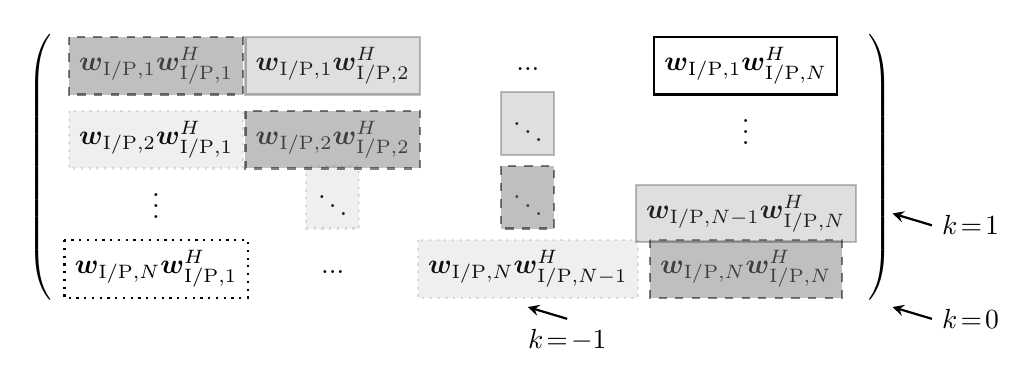
\begin{tikzpicture}[>=stealth,thick,baseline,every right delimiter/.append style={name=rd},]
						\matrix [matrix of math nodes,left delimiter=(,right delimiter=)] (m)
						{
							\boldsymbol{w}_{\mathrm{I/P},1}\boldsymbol{w}_{\mathrm{I/P},1}^H & \boldsymbol{w}_{\mathrm{I/P},1}\boldsymbol{w}_{\mathrm{I/P},2}^H & \dots & \boldsymbol{w}_{\mathrm{I/P},1}\boldsymbol{w}_{\mathrm{I/P},N}^H \\
							\boldsymbol{w}_{\mathrm{I/P},2}\boldsymbol{w}_{\mathrm{I/P},1}^H & \boldsymbol{w}_{\mathrm{I/P},2}\boldsymbol{w}_{\mathrm{I/P},2}^H & \ddots & \vdots \\
							\vdots & \ddots & \ddots & \boldsymbol{w}_{\mathrm{I/P},N-1}\boldsymbol{w}_{\mathrm{I/P},N}^H \\
							\boldsymbol{w}_{\mathrm{I/P},N}\boldsymbol{w}_{\mathrm{I/P},1}^H & \dots & \boldsymbol{w}_{\mathrm{I/P},N}\boldsymbol{w}_{\mathrm{I/P},N-1}^H & \boldsymbol{w}_{\mathrm{I/P},N}\boldsymbol{w}_{\mathrm{I/P},N}^H \\
						};
						\draw[dotted,thick] (m-4-1.north west) rectangle (m-4-1.south east);
						\draw[dotted,thick,fill=gray,opacity=0.125] (m-2-1.north west) rectangle (m-2-1.south east); \draw[dotted,thick,fill=gray,opacity=0.125] (m-3-2.north west) rectangle (m-3-2.south east); \draw[dotted,thick,fill=gray,opacity=0.125] (m-4-3.north west) rectangle (m-4-3.south east);
						\draw[dashed,thick,fill=gray,opacity=0.5] (m-1-1.north west) rectangle (m-1-1.south east); \draw[dashed,thick,fill=gray,opacity=0.5] (m-2-2.north west) rectangle (m-2-2.south east); \draw[dashed,thick,fill=gray,opacity=0.5] (m-3-3.north west) rectangle (m-3-3.south east); \draw[dashed,thick,fill=gray,opacity=0.5] (m-4-4.north west) rectangle (m-4-4.south east);
						\draw[solid,thick,fill=gray,opacity=0.25] (m-1-2.north west) rectangle (m-1-2.south east); \draw[solid,thick,fill=gray,opacity=0.25] (m-2-3.north west) rectangle (m-2-3.south east); \draw[solid,thick,fill=gray,opacity=0.25] (m-3-4.north west) rectangle (m-3-4.south east);
						\draw[solid,thick] (m-1-4.north west) rectangle (m-1-4.south east);
						\draw[<-] (m-4-3.south|-m.south) -- ++(0.5,-0.15) node[below]{$k=-1$};
						\draw[<-] (rd.east|-m.south) -- ++(0.5,-0.15) node[right]{$k=0$};
						\draw[<-] (rd.east|-m-3-4.east) -- ++(0.5,-0.15) node[right]{$k=1$};
					\end{tikzpicture}
				\end{equation*}
				\caption{$\boldsymbol{W}_{\mathrm{I/P}}$ consists of $N \times N$ blocks of size $M \times M$. $\boldsymbol{W}_{\mathrm{I/P},k}$ keeps the $k$-th block diagonal of $\boldsymbol{W}_{\mathrm{I/P}}$ and nulls all remaining blocks. Solid, dashed and dotted blocks correspond to $k>0$, $k=0$ and $k<0$, respectively. For $\boldsymbol{w}_{\mathrm{I/P},n_1}\boldsymbol{w}_{\mathrm{I/P},n_2}^H$, the $k$-th block diagonal satisfies $k=n_2-n_1$.}
				\label{fi:block_diagonal}
			\end{figure*}

			\begin{figure*}[!b]
				\hrule
				\begin{align}
					&z(\boldsymbol{\phi},\boldsymbol{w}_{\mathrm{I}},\boldsymbol{w}_{\mathrm{P}},\rho) = \beta_2\rho\Bigl(\mathbb{E}\left\{\mathbb{A}\left\{y_{\mathrm{I}}^2(t)\right\}\right\}+\mathbb{A}\left\{y_{\mathrm{P}}^2(t)\right\}\Bigr)+\beta_4\rho^2\Bigl(\mathbb{E}\left\{\mathbb{A}\left\{y_{\mathrm{I}}^4(t)\right\}\right\}+\mathbb{A}\left\{y_{\mathrm{P}}^4(t)\right\}+6\mathbb{E}\left\{\mathbb{A}\left\{y_{\mathrm{I}}^2(t)\right\}\right\}\mathbb{A}\left\{y_{\mathrm{P}}^2(t)\right\}\Bigr),\label{eq:z_expand}\\
					&\mathbb{E}\left\{\mathbb{A}\left\{y_{\mathrm{I}}^2(t)\right\}\right\} = \frac{1}{2}\sum_{n=1}^N{(\boldsymbol{h}_{n}^H\boldsymbol{w}_{\mathrm{I},n})(\boldsymbol{h}_{n}^H\boldsymbol{w}_{\mathrm{I},n})^*} = \frac{1}{2}\boldsymbol{h}^H\boldsymbol{W}_{\mathrm{I},0}\boldsymbol{h},\label{eq:y_I2}\\
					&\mathbb{E}\left\{\mathbb{A}\left\{y_{\mathrm{I}}^4(t)\right\}\right\} = \frac{3}{4}\left(\sum_{n=1}^N{(\boldsymbol{h}_{n}^H\boldsymbol{w}_{\mathrm{I},n})(\boldsymbol{h}_{n}^H\boldsymbol{w}_{\mathrm{I},n})^*}\right)^2 = \frac{3}{4}(\boldsymbol{h}^H\boldsymbol{W}_{\mathrm{I},0}\boldsymbol{h})^2,\label{eq:y_I4}\\
					&\mathbb{A}\left\{y_{\mathrm{P}}^2(t)\right\} = \frac{1}{2}\sum_{n=1}^N{(\boldsymbol{h}_{n}^H\boldsymbol{w}_{\mathrm{P},n})(\boldsymbol{h}_{n}^H\boldsymbol{w}_{\mathrm{P},n})^*} = \frac{1}{2}\boldsymbol{h}^H\boldsymbol{W}_{\mathrm{P},0}\boldsymbol{h},\label{eq:y_P2}\\
					&\mathbb{A}\left\{y_{\mathrm{P}}^4(t)\right\} = \frac{3}{8}\sum_{\substack{{n_1},{n_2},{n_3},{n_4}\\{n_1}+{n_2}={n_3}+{n_4}}}{(\boldsymbol{h}_{{n_1}}^H\boldsymbol{w}_{\mathrm{P},{n_1}})(\boldsymbol{h}_{{n_2}}^H\boldsymbol{w}_{\mathrm{P},{n_2}})(\boldsymbol{h}_{{n_3}}^H\boldsymbol{w}_{\mathrm{P},{n_3}})^*(\boldsymbol{h}_{{n_4}}^H\boldsymbol{w}_{\mathrm{P},{n_4}})^*} = \frac{3}{8}\sum_{k=-N+1}^{N-1}(\boldsymbol{h}^H\boldsymbol{W}_{\mathrm{P},k}\boldsymbol{h})(\boldsymbol{h}^H\boldsymbol{W}_{\mathrm{P},k}\boldsymbol{h})^*.\label{eq:y_P4}
				\end{align}
			\end{figure*}
		\end{subsection}


		\begin{subsection}{Rate-Energy Region}
			The achievable R-E region is defined as
			\begin{align}
				\mathcal{C}_{\mathrm{R-E}}
				&\triangleq \biggl\{(R_{\mathrm{ID}}, z_{\mathrm{EH}}) \in \mathbb{R}_+^2 \mid R_{\mathrm{ID}} \le R, z_{\mathrm{EH}} \le z,\nonumber\\
				&\quad \frac{1}{2}\left(\lVert{\boldsymbol{w}_{\mathrm{I}}}\rVert^2+\lVert{\boldsymbol{w}_{\mathrm{P}}}\rVert^2\right) \le P\biggr\},
			\end{align}
			where $P$ is the average transmit power budget and \num{1/2} converts the peak value of sine waves to the average value.
		\end{subsection}
	\end{section}


	\begin{section}{Problem Formulation}\label{se:problem_formulation}
		We characterize each R-E boundary point through a current maximization problem subject to sum rate, transmit power, and IRS magnitude constraints as
		\begin{maxi!}
			{\scriptstyle{\boldsymbol{\phi},\boldsymbol{w}_{\mathrm{I}},\boldsymbol{w}_{\mathrm{P}},\rho}}{z(\boldsymbol{\phi},\boldsymbol{w}_{\mathrm{I}},\boldsymbol{w}_{\mathrm{P}},\rho)}{\label{op:original}}{\label{ob:original}}
			\addConstraint{R(\boldsymbol{\phi},\boldsymbol{w}_{\mathrm{I}},\rho) \ge \bar{R}}\label{co:original_rate}
			\addConstraint{\frac{1}{2}\left(\lVert{\boldsymbol{w}_{\mathrm{I}}}\rVert^2+\lVert{\boldsymbol{w}_{\mathrm{P}}}\rVert^2\right)\le{P}}\label{co:original_power}
			\addConstraint{\lvert{\boldsymbol{\phi}}\rvert=\boldsymbol{1}}\label{co:original_modulus}
			\addConstraint{0 \le \rho \le 1.}
		\end{maxi!}
		Problem~\eqref{op:original} is intricate due to the coupled variables in \eqref{ob:original}, \eqref{co:original_rate} and the non-convex constraint \eqref{co:original_modulus}. To obtain a feasible solution, we propose a BCD algorithm that iteratively updates 1) the IRS phase shift, 2) the active precoder, 3) the waveform amplitude and splitting ratio, until convergence.


		\begin{subsection}{Passive Beamforming}
			In this section, we optimize the IRS phase shift $\boldsymbol{\phi}$ for any given waveform $\boldsymbol{w}_{\mathrm{I/P}}$ and splitting ratio $\rho$. Note that
			\begin{align}
				\lvert \boldsymbol{h}_{n}^H\boldsymbol{w}_{\mathrm{I},n} \rvert^2
				& = \boldsymbol{w}_{\mathrm{I},n}^H\boldsymbol{h}_n\boldsymbol{h}_n^H\boldsymbol{w}_{\mathrm{I},n}\nonumber\\
				& = \boldsymbol{w}_{\mathrm{I},n}^H(\boldsymbol{h}_{\mathrm{D},n}+\boldsymbol{V}_n^H\boldsymbol{\phi})(\boldsymbol{h}_{\mathrm{D},n}^H+\boldsymbol{\phi}^H\boldsymbol{V}_n)\boldsymbol{w}_{\mathrm{I},n}\nonumber\\
				& = \boldsymbol{w}_{\mathrm{I},n}^H\boldsymbol{M}_n^H\boldsymbol{\Phi}\boldsymbol{M}_n\boldsymbol{w}_{\mathrm{I},n}\nonumber\\
				& = \mathrm{tr}(\boldsymbol{M}_n\boldsymbol{w}_{\mathrm{I},n}\boldsymbol{w}_{\mathrm{I},n}^H\boldsymbol{M}_n^H\boldsymbol{\Phi})\nonumber\\
				& = \mathrm{tr}(\boldsymbol{C}_n\boldsymbol{\Phi}),
			\end{align}
			where $\boldsymbol{M}_n \triangleq [\boldsymbol{V}_n^H, \boldsymbol{h}_{\mathrm{D},n}]^H \in \mathbb{C}^{(L+1) \times M}$, $t'$ is an auxiliary variable with unit modulus, $\bar{\boldsymbol{\phi}} \triangleq [\boldsymbol{\phi}^H, t']^H \in \mathbb{C}^{(L+1) \times 1}$, $\boldsymbol{\Phi} \triangleq \bar{\boldsymbol{\phi}}\bar{\boldsymbol{\phi}}^H \in \mathbb{C}^{(L+1) \times (L+1)}$, $\boldsymbol{C}_n \triangleq \boldsymbol{M}_n\boldsymbol{w}_{\mathrm{I},n}\boldsymbol{w}_{\mathrm{I},n}^H\boldsymbol{M}_n^H \in \mathbb{C}^{(L+1)\times(L+1)}$. On the other hand, we define $t_{\mathrm{I/P},k}$ as
			\begin{align}
				t_{\mathrm{I/P},k}
				& \triangleq \boldsymbol{h}^H\boldsymbol{W}_{\mathrm{I/P},k}\boldsymbol{h}\nonumber\\
				& = \mathrm{tr}(\boldsymbol{h}\boldsymbol{h}^H\boldsymbol{W}_{\mathrm{I/P},k})\nonumber\\
				& = \mathrm{tr}\left((\boldsymbol{h}_{D}+\boldsymbol{V}^H\boldsymbol{\phi})(\boldsymbol{h}_{D}^H+\boldsymbol{\phi}^H\boldsymbol{V})\boldsymbol{W}_{\mathrm{I/P},k}\right)\nonumber\\
				& = \mathrm{tr}(\boldsymbol{M}^H\boldsymbol{\Phi}\boldsymbol{M}\boldsymbol{W}_{\mathrm{I/P},k})\nonumber\\
				& = \mathrm{tr}(\boldsymbol{M}\boldsymbol{W}_{\mathrm{I/P},k}\boldsymbol{M}^H\boldsymbol{\Phi})\nonumber\\
				& = \mathrm{tr}(\boldsymbol{C}_{\mathrm{I/P},k}\boldsymbol{\Phi})\label{eq:t_k},
			\end{align}
			where $\boldsymbol{V} \triangleq [\boldsymbol{V}_1,\dots,\boldsymbol{V}_N] \in \mathbb{C}^{L \times MN}$, $\boldsymbol{M} \triangleq [\boldsymbol{V}^H, \boldsymbol{h}_{D}]^H \in \mathbb{C}^{(L+1) \times MN}$, $\boldsymbol{C}_{\mathrm{I/P},k} \triangleq \boldsymbol{M}\boldsymbol{W}_{\mathrm{I/P},k}\boldsymbol{M}^H \in \mathbb{C}^{(L+1)\times(L+1)}$. On top of this, \eqref{eq:R} and \eqref{eq:z_expand} reduce respectively to
			\begin{align}
				R(\boldsymbol{\Phi})
				& = \sum_{n=1}^{N}{\log_2\left(1+\frac{(1-\rho)\mathrm{tr}(\boldsymbol{C}_n\boldsymbol{\Phi})}{\sigma_n^2}\right)},\label{eq:R_irs}\\
				z(\boldsymbol{\Phi})
				& = \frac{1}{2}{\beta_2}{\rho}(t_{\mathrm{I},0}+t_{\mathrm{P},0})\nonumber\\
				& \quad + \frac{3}{8}{\beta_4}{\rho^2} \left(2t_{\mathrm{I},0}^2 + \sum_{k=-N+1}^{N-1}{t_{\mathrm{P},k}t_{\mathrm{P},k}^*}\right)\nonumber\\
				& \quad + \frac{3}{2}{\beta_4}{\rho^2}t_{\mathrm{I},0}t_{\mathrm{P},0}.\label{eq:z_irs}
			\end{align}
			To maximize the non-concave expression \eqref{eq:z_irs}, we successively lower bound the second-order terms by their first-order Taylor expansions \cite{Adali2010}. Based on the solution at iteration $i - 1$, the approximations at iteration $i$ are
			\begin{align}
				(t_{\mathrm{I},0}^{(i)})^2
				& \ge 2 t_{\mathrm{I},0}^{(i)}t_{\mathrm{I},0}^{(i-1)} - (t_{\mathrm{I},0}^{(i-1)})^2,\label{eq:taylor_1}\\
				t_{\mathrm{P},k}^{(i)} (t_{\mathrm{P},k}^{(i)})^*
				& \ge 2 \Re\left\{t_{\mathrm{P},k}^{(i)} (t_{\mathrm{P},k}^{(i-1)})^*\right\} - t_{\mathrm{P},k}^{(i-1)} (t_{\mathrm{P},k}^{(i-1)})^*,\label{eq:taylor_2}\\
				t_{\mathrm{I},0}^{(i)} t_{\mathrm{P},0}^{(i)}
				& \ge t_{\mathrm{I},0}^{(i)} t_{\mathrm{P},0}^{(i-1)} + t_{\mathrm{P},0}^{(i)} t_{\mathrm{I},0}^{(i-1)} - t_{\mathrm{I},0}^{(i-1)} t_{\mathrm{P},0}^{(i-1)}.\label{eq:taylor_3}
			\end{align}
			Note that $t_{\mathrm{I/P},0}=\mathrm{tr}(\boldsymbol{C}_{\mathrm{I/P},0}\boldsymbol{\Phi})$ is real because $\boldsymbol{C}_{\mathrm{I/P},0}$ and $\boldsymbol{\Phi}$ are Hermitian matrices. Due to symmetry \cite{Huang2017}, we have
			\begin{equation}\label{eq:coupled_terms}
				\sum_{k=-N+1}^{N-1} \Re\left\{t_{\mathrm{P},k}^{(i)} (t_{\mathrm{P},k}^{(i-1)})^*\right\} = \sum_{k=-N+1}^{N-1} t_{\mathrm{P},k}^{(i)} (t_{\mathrm{P},k}^{(i-1)})^*.
			\end{equation}
			Plugging \eqref{eq:taylor_1}--\eqref{eq:coupled_terms} into \eqref{eq:z_irs}, we obtain the DC current approximation $\tilde{z}$ as \eqref{eq:z_irs_approx} and transform problem~\eqref{op:original} to
			\begin{figure*}[!b]
				\hrule
				\begin{align}
					\tilde{z}(\boldsymbol{\Phi}^{(i)})
					& = \frac{1}{2}{\beta_2}{\rho}(t_{\mathrm{I},0}^{(i)}+t_{\mathrm{P},0}^{(i)}) + \frac{3}{8}{\beta_4}{\rho^2} \left(4 t_{\mathrm{I},0}^{(i)}t_{\mathrm{I},0}^{(i-1)} - 2 (t_{\mathrm{I},0}^{(i-1)})^2 + \sum_{k=-N+1}^{N-1}{2 t_{\mathrm{P},k}^{(i)} (t_{\mathrm{P},k}^{(i-1)})^* - t_{\mathrm{P},k}^{(i-1)} (t_{\mathrm{P},k}^{(i-1)})^*}\right)\nonumber\\
					& \quad + \frac{3}{2}{\beta_4}{\rho^2} \left(t_{\mathrm{I},0}^{(i)} t_{\mathrm{P},0}^{(i-1)} + t_{\mathrm{P},0}^{(i)} t_{\mathrm{I},0}^{(i-1)} - t_{\mathrm{I},0}^{(i-1)} t_{\mathrm{P},0}^{(i-1)}\right).\label{eq:z_irs_approx}
				\end{align}
			\end{figure*}
			\begin{maxi!}
				{\scriptstyle{\boldsymbol{\Phi}}}{\tilde{z}(\boldsymbol{\Phi})}{\label{op:irs}}{\label{ob:irs}}
				\addConstraint{R(\boldsymbol{\Phi}) \ge \bar{R}}\label{co:irs_rate}
				\addConstraint{\mathrm{diag}^{-1}(\boldsymbol{\Phi})=\boldsymbol{1}}\label{co:irs_modulus}
				\addConstraint{\boldsymbol{\Phi}\succeq{\boldsymbol{0}}}\label{co:irs_sd}
				\addConstraint{\mathrm{rank}(\boldsymbol{\Phi})=1.\label{co:irs_rank}}
			\end{maxi!}
			We then apply Semi-Definite Relaxation (SDR) to the unit-rank constraint \eqref{co:irs_rank} and formulate a Semi-Definite Programming (SDP) with approximation accuracy no greater than $\pi/4$ \cite{Luo2010}. In this specific case, we found the solution provided by CVX toolbox \cite{Grant2008} to \eqref{ob:irs}-\eqref{co:irs_sd} is always rank-\num{1}. This conclusion is summarized below.

			\begin{proposition}\label{pr:relaxation}
				Any optimal solution $\boldsymbol{\Phi}^\star$ to the relaxed passive beamforming problem~\eqref{ob:irs}--\eqref{co:irs_sd} is rank-\num{1} such that \eqref{co:irs_rank} is tight and no loss is introduced by SDR.
			\end{proposition}

			\begin{proof}\label{pf:relaxation}
				Please refer to Appendix~\ref{ap:relaxation}.
			\end{proof}

			In summary, we update $\boldsymbol{\Phi}^{(i)}$ until convergence, extract $\hat{\boldsymbol{\phi}}^\star$ by eigen decomposition, and retrieve the	IRS vector by $\boldsymbol{\phi}^{\star}=e^{j \arg\left([\hat{\boldsymbol{\phi}}^\star]_{(1:L)} \middle/ [\hat{\boldsymbol{\phi}}^\star]_{(L+1)}\right)}$. The passive beamforming design is summarized in the SCA Algorithm~\ref{al:sca}, where the relaxed problem \eqref{ob:irs}--\eqref{co:irs_sd} involves a $(L+1)$-order positive semi-definite matrix variable and $(L+2)$ linear constraints. Given a solution accuracy $\epsilon_{\mathrm{IPM}}$ for the interior-point method, the computational complexity of Algorithm~\ref{al:sca} is $\mathcal{O}\left(I_{\mathrm{SCA}}(L+2)^4 (L+1)^{0.5} \log(\epsilon_{\mathrm{IPM}}^{-1})\right)$, where $I_{\mathrm{SCA}}$ denotes the number of SCA iterations \cite{Luo2010}.

			\begin{algorithm}[!t]
				\caption{SCA: IRS Phase Shift.}
				\label{al:sca}
				\begin{algorithmic}[1]
					\State \textbf{Input} $\beta_2$, $\beta_4$, $\boldsymbol{h}_{\mathrm{D},n}$, $\boldsymbol{V}_{n}$, $\sigma_n$, $\boldsymbol{w}_{\mathrm{I/P},n}$, $\rho$, $\bar{R}$, $\epsilon$, $\forall n$
					\State Construct $\boldsymbol{V}$, $\boldsymbol{M}$, $\boldsymbol{M}_n$, $\boldsymbol{C}_{n}$, $\boldsymbol{C}_{\mathrm{I/P},k}$, $\forall n,k$
					\State \textbf{Initialize} $i \gets 0$, $\boldsymbol{\Phi}^{(0)}$
					\State Set $t_{\mathrm{I/P},k}^{(0)}$, $\forall k$ by \eqref{eq:t_k}
					\State Compute $z^{(0)}$ by \eqref{eq:z_irs}
					\Repeat
						\State $i \gets i + 1$
						\State Get $\boldsymbol{\Phi}^{(i)}$ by solving \eqref{ob:irs}--\eqref{co:irs_sd}
						\State Update $t_{\mathrm{I/P},k}^{(i)}$, $\forall k$ by \eqref{eq:t_k}
						\State Compute $z^{(i)}$ by \eqref{eq:z_irs}
					\Until $\lvert z^{(i)}-z^{(i-1)} \rvert \le \epsilon$
					\State Set $\boldsymbol{\Phi}^{\star}=\boldsymbol{\Phi}^{(i)}$
					\State Get $\hat{\boldsymbol{\phi}}^\star$ by eigen decomposition, $\boldsymbol{\Phi}^{\star}=\hat{\boldsymbol{\phi}}^\star(\hat{\boldsymbol{\phi}}^\star)^H$
					\State Set $\boldsymbol{\phi}^{\star}=e^{j \arg\left([\hat{\boldsymbol{\phi}}^\star]_{(1:L)} \middle/ [\hat{\boldsymbol{\phi}}^\star]_{(L+1)}\right)}$
					\State \textbf{Output} $\boldsymbol{\phi}^{\star}$
				\end{algorithmic}
			\end{algorithm}

			\begin{proposition}\label{pr:sca}
				For any feasible initial point with given waveform and splitting ratio, the SCA Algorithm~\ref{al:sca} is guaranteed to converge to local optimal points of the original problem~\eqref{op:original}.
			\end{proposition}

			\begin{proof}\label{pf:sca}
				Please refer to Appendix~\ref{ap:sca}.
			\end{proof}
		\end{subsection}

		\begin{subsection}{Active Beamforming}
			To avoid straightforward optimization over complex vectors $\boldsymbol{w}_{\mathrm{I/P}}$ of size $MN \times 1$, we decouple the waveform in the spatial and frequency domains to reduce the size of variables. The weight on subband $n$ is essentially
			\begin{equation}\label{eq:w}
				\boldsymbol{w}_{\mathrm{I/P}, n} = s_{\mathrm{I/P}, n} \boldsymbol{b}_{\mathrm{I/P}, n},
			\end{equation}
			where $s_{\mathrm{I/P},n}$ denotes the amplitude of the modulated/multisine waveform at tone $n$, and $\boldsymbol{b}_{\mathrm{I/P}, n}$ denotes the corresponding information/power precoder. Define $\boldsymbol{s}_{\mathrm{I/P}} \triangleq [s_{\mathrm{I/P},1},\dots,s_{\mathrm{I/P},N}]^T \in \mathbb{R}_+^{N \times 1}$. The MRT precoder at subband $n$ is given by
			\begin{equation}\label{eq:b_n}
				\boldsymbol{b}_{\mathrm{I/P}, n}^\star = \frac{\boldsymbol{h}_n}{\lVert{\boldsymbol{h}_n}\rVert}.
			\end{equation}

			\begin{proposition}\label{pr:mrt}
				For single-user SWIPT, the global optimal information and power precoders coincide at the MRT.
			\end{proposition}

			\begin{proof}\label{pf:mrt}
				Please refer to Appendix~\ref{ap:mrt}.
			\end{proof}
		\end{subsection}


		\begin{subsection}{Waveform and Splitting Ratio}
			Next, we jointly optimize the waveform amplitude $\boldsymbol{s}_{\mathrm{I/P}}$ and the splitting ratio $\rho$ for any given IRS phase shift $\boldsymbol{\phi}$ and active precoder $\boldsymbol{b}_{\mathrm{I/P},n}$, $\forall n$. On top of \eqref{eq:b_n}, the equivalent channel strength at subband $n$ is $\lVert{\boldsymbol{h}_n}\rVert$ and the rate \eqref{eq:R} reduces to
			\begin{equation}\label{eq:R_waveform}
				R(\boldsymbol{s}_{\mathrm{I}},\rho) = \log_2\prod_{n=1}^N\left(1+\frac{(1-\rho)\lVert{\boldsymbol{h}_n}\rVert^2 s_{\mathrm{I},n}^2}{\sigma_n^2}\right),
			\end{equation}
			and the DC current \eqref{eq:z_expand} rewrites as \eqref{eq:z_waveform}, so that problem~\eqref{op:original} boils down to
			\begin{figure*}[!b]
				\begin{align}
					z(\boldsymbol{s}_{\mathrm{I}},\boldsymbol{s}_\mathrm{P},\rho)
					& = \frac{1}{2}{\beta_2}{\rho} \sum_{n=1}^N \lVert{\boldsymbol{h}_n}\rVert^2(s_{\mathrm{I},n}^2+s_{\mathrm{P},n}^2) + \frac{3}{8}{\beta_4}{\rho^2} \left( 2\sum_{n_1,n_2} \prod_{j=1}^2 \lVert{\boldsymbol{h}_{n_j}}\rVert^2 s_{\mathrm{I},{n_j}}^2 + \sum_{\substack{{n_1},{n_2},{n_3},{n_4}\\{n_1}+{n_2}={n_3}+{n_4}}} \prod_{j=1}^4 \lVert{\boldsymbol{h}_{n_j}}\rVert s_{\mathrm{P},{n_j}} \right)\nonumber\\
					& \quad + \frac{3}{2}{\beta_4}{\rho^2} \left( \sum_{n_1,n_2} \lVert{\boldsymbol{h}_{n_1}}\rVert^2 \lVert{\boldsymbol{h}_{n_2}}\rVert^2 s_{\mathrm{I},{n_1}}^2 s_{\mathrm{P},{n_2}}^2 \right).\label{eq:z_waveform}
				\end{align}
			\end{figure*}
			\begin{maxi!}
				{\scriptstyle{\boldsymbol{s}_{\mathrm{I}},\boldsymbol{s}_\mathrm{P},\rho}}{z(\boldsymbol{s}_{\mathrm{I}},\boldsymbol{s}_\mathrm{P},\rho)}{\label{op:waveform}}{}
				\addConstraint{R(\boldsymbol{s}_{\mathrm{I}},\rho) \ge \bar{R}}
				\addConstraint{\frac{1}{2}\left(\lVert{\boldsymbol{s}_{\mathrm{I}}}\rVert^2+\lVert{\boldsymbol{s}_\mathrm{P}}\rVert^2\right)\le{P}.}
			\end{maxi!}
			Following \cite{Clerckx2018b}, we introduce auxiliary variables $t'',\bar{\rho}$\footnote{It can be concluded $\bar{\rho}^{\star}=1-\rho^{\star}$ because the R-E tradeoff is maximized when no signal component is wasted at the receiver.} and transform problem~\eqref{op:waveform} into a reversed GP
			\begin{mini!}
				{\scriptstyle{\boldsymbol{s}_{\mathrm{I}},\boldsymbol{s}_\mathrm{P},\rho,\bar{\rho},t''}}{\frac{1}{t''}}{\label{op:waveform_rgp}}{}
				\addConstraint{\frac{t''}{z(\boldsymbol{s}_{\mathrm{I}},\boldsymbol{s}_\mathrm{P},\rho)} \le 1}\label{co:waveform_objective}
				\addConstraint{\frac{2^{\bar{R}}}{\prod_{n=1}^N \left(1+{\bar{\rho}\lVert{\boldsymbol{h}_n}\rVert^2 s_{\mathrm{I},n}^2}\big/{\sigma_n^2}\right)} \le 1}\label{co:waveform_rate}
				\addConstraint{\frac{1}{2}\left(\lVert{\boldsymbol{s}_{\mathrm{I}}}\rVert^2+\lVert{\boldsymbol{s}_\mathrm{P}}\rVert^2\right) \le P}\label{co:waveform_power}
				\addConstraint{\rho + \bar{\rho} \le 1.}\label{co:waveform_splitting_ratio}
			\end{mini!}
			The denominators of \eqref{co:waveform_rate} and \eqref{co:waveform_objective} consist of posynomials \cite{Boyd2007} that can be decomposed as sums of monomials
			\begin{align}
				1+\frac{\bar{\rho}\lVert{\boldsymbol{h}_n}\rVert^2 s_{\mathrm{I},n}^2}{\sigma_n^2} &\triangleq \sum_{m_{\mathrm{I},n}}g_{m_{\mathrm{I},n}}(s_{\mathrm{I},n},\bar{\rho})\label{eq:g_I},\\
				z(\boldsymbol{s}_{\mathrm{I}},\boldsymbol{s}_\mathrm{P},\rho) &\triangleq \sum_{m_\mathrm{P}}{g_{m_\mathrm{P}}(\boldsymbol{s}_{\mathrm{I}},\boldsymbol{s}_\mathrm{P},\rho)}\label{eq:g_P},
			\end{align}
			where $m_{\mathrm{I},n}=2$ and $m_\mathrm{P}=(2N^3+6N^2+7N)/3$. We upper bound \eqref{eq:g_I} and \eqref{eq:g_P} by the Arithmetic Mean-Geometric Mean (AM-GM) inequality \cite{Chiang2005} and transform problem~\eqref{op:waveform_rgp} to
			\begin{mini!}
				{\scriptstyle{\boldsymbol{s}_{\mathrm{I}},\boldsymbol{s}_\mathrm{P},\rho,\bar{\rho},t''}}{\frac{1}{t''}}{\label{op:waveform_gp}}{}
				\addConstraint{{t''}\prod_{m_\mathrm{P}}{\left(\frac{g_{{m_\mathrm{P}}}(\boldsymbol{s}_{\mathrm{I}},\boldsymbol{s}_\mathrm{P},\rho)}{\gamma_{{m_\mathrm{P}}}}\right)^{-\gamma_{{m_\mathrm{P}}}}}\le{1}}
				\addConstraint{2^{\bar{R}}\prod_{n}\prod_{m_{\mathrm{I},n}}\left(\frac{g_{m_{\mathrm{I},n}}(s_{\mathrm{I},n},\bar{\rho})}{\gamma_{m_{\mathrm{I},n}}}\right)^{-\gamma_{m_{\mathrm{I},n}}}\le{1}}
				\addConstraint{\frac{1}{2}\left(\lVert{\boldsymbol{s}_{\mathrm{I}}}\rVert^2+\lVert{\boldsymbol{s}_\mathrm{P}}\rVert^2\right)\le{P}}
				\addConstraint{\rho + \bar{\rho} \le 1,}
			\end{mini!}
			where $\gamma_{m_{\mathrm{I},n}} \ge 0$, $\gamma_{m_\mathrm{P}} \ge 0$, $\sum_{m_{\mathrm{I},n}}\gamma_{m_{\mathrm{I},n}}=\sum_{m_\mathrm{P}}\gamma_{m_\mathrm{P}}=1$. The tightness of the AM-GM inequality depends on $\{\gamma_{m_{\mathrm{I},n}},\gamma_{m_\mathrm{P}}\}$, and a feasible choice at iteration $i$ is
			\begin{align}
				\gamma_{m_{\mathrm{I},n}}^{(i)} & = \frac{g_{m_{\mathrm{I},n}}(s_{\mathrm{I},n}^{(i-1)},\bar{\rho}^{(i-1)})}{1+{\bar{\rho}^{(i-1)}\lVert{\boldsymbol{h}_n}\rVert^2 (s_{\mathrm{I},n}^{(i-1)})^2}\big/{\sigma_n^2}}\label{eq:gamma_I},\\
				\gamma_{m_\mathrm{P}}^{(i)} & = \frac{g_{m_\mathrm{P}}(\boldsymbol{s}_{\mathrm{I}}^{(i-1)},\boldsymbol{s}_\mathrm{P}^{(i-1)},\rho^{(i-1)})}{z(\boldsymbol{s}_{\mathrm{I}}^{(i-1)},\boldsymbol{s}_\mathrm{P}^{(i-1)},\rho^{(i-1)})}\label{eq:gamma_P}.
			\end{align}
			With \eqref{eq:gamma_I} and \eqref{eq:gamma_P}, problem~\eqref{op:waveform_gp} can be solved by existing optimization tools such as CVX \cite{Grant2008}. We update $\boldsymbol{s}_{\mathrm{I}}^{(i)},\boldsymbol{s}_\mathrm{P}^{(i)},\rho^{(i)}$ iteratively until convergence. The joint waveform amplitude and splitting ratio design is summarized in the GP Algorithm~\ref{al:gp}, which achieves local optimality at the cost of exponential computational complexity \cite{Chiang2005}.

			\begin{algorithm}[!t]
				\caption{GP: Waveform Amplitude and Splitting Ratio.}
				\label{al:gp}
				\begin{algorithmic}[1]
					\State \textbf{Input} $\beta_2$, $\beta_4$, $\boldsymbol{h}_n$, $P$, $\sigma_n$, $\bar{R}$, $\epsilon$, $\forall n$
					\State \textbf{Initialize} $i \gets 0$, $\boldsymbol{s}_{\mathrm{I/P}}^{(0)}$, $\rho^{(0)}$
					\State Compute $R^{(0)}$, $z^{(0)}$ by \eqref{eq:R_waveform}, \eqref{eq:z_waveform}
					\State Set $g_{m_{\mathrm{I},n}}^{(0)}$, $g_{m_\mathrm{P}}^{(0)}$, $\forall n$ by \eqref{eq:g_I}, \eqref{eq:g_P}
					\Repeat
						\State $i \gets i + 1$
						\State Update $\gamma_{m_{\mathrm{I},n}}^{(i)}$, $\gamma_{m_\mathrm{P}}^{(i)}$, $\forall n$ by \eqref{eq:gamma_I}, \eqref{eq:gamma_P}
						\State Get $\boldsymbol{s}_{\mathrm{I/P}}^{(i)}$, $\rho^{(i)}$ by solving problem~\eqref{op:waveform_gp}
						\State Compute $R^{(i)}$, $z^{(i)}$ by \eqref{eq:R_waveform}, \eqref{eq:z_waveform}
						\State Update $g_{m_{\mathrm{I},n}}^{(i)}$, $g_{m_\mathrm{P}}^{(i)}$, $\forall n$ by \eqref{eq:g_I}, \eqref{eq:g_P}
					\Until $\lvert z^{(i)} - z^{(i-1)} \rvert \le \epsilon$
					\State Set $\boldsymbol{s}_{\mathrm{I/P}}^{\star}=\boldsymbol{s}_{\mathrm{I/P}}^{(i)}$, $\rho^{\star}=\rho^{(i)}$
					\State \textbf{Output} $\boldsymbol{s}_{\mathrm{I}}^{\star}$, $\boldsymbol{s}_{\mathrm{P}}^{\star}$, $\rho^{\star}$
				\end{algorithmic}
			\end{algorithm}

			\begin{proposition}\label{pr:gp}
				For any feasible initial point, the GP Algorithm~\ref{al:gp} is guaranteed to converge to local optimal points of the waveform amplitude and splitting ratio design problem \eqref{op:waveform}.
			\end{proposition}

			\begin{proof}\label{pf:gp}
				Please refer to \cite{Clerckx2016a,Clerckx2018b}.
			\end{proof}
		\end{subsection}


		\begin{subsection}{Low-Complexity Adaptive Design}
			To facilitate practical SWIPT implementation, we propose two closed-form adaptive waveform amplitude schemes by combining WF and SMF in the time and power domains. For WIT, the optimal WF strategy assigns the amplitude of modulated tone $n$ by
			\begin{equation}\label{eq:wf}
				s_{\mathrm{I}, n} = \sqrt{2\left(\lambda - \frac{\sigma_n^2}{P \lVert{\boldsymbol{h}_n}\rVert^2}\right)^+},
			\end{equation}
			where $\lambda$ is chosen to satisfy the power constraint $\lVert{\boldsymbol{s}_I}\rVert^2 / 2 \le P$. The closed-form solution can be obtained by iterative power allocation \cite{Tse2005}, and the details are omitted here. On the other hand, SMF was proposed in \cite{Clerckx2017} as a suboptimal WPT resource allocation scheme that assigns the amplitude of sinewave $n$ by
			\begin{equation}\label{eq:smf}
				s_{\mathrm{P}, n} = \sqrt{\frac{2 P}{\sum_{n=1}^N \lVert{\boldsymbol{h}_n \rVert^{2 \alpha}}}}\lVert{\boldsymbol{h}_n}\rVert^\alpha,
			\end{equation}
			where the scaling ratio $\alpha \ge 1$ is given and can be adjusted to exploit the rectifier nonlinearity and frequency selectivity. When the receiver works in TS mode, there is no superposition in the suboptimal waveform design. Modulated waveform with amplitude \eqref{eq:wf} is used in the data session while multisine waveform with amplitude \eqref{eq:smf} is used in the energy session. When the receiver works in PS mode, we jointly design the combining ratio $\delta$ with the splitting ratio $\rho$, and assign the superposed waveform amplitudes as
			\begin{align}
				s_{\mathrm{I}, n} &= \sqrt{2(1 - \delta)\left(\lambda - \frac{\sigma_n^2}{P \lVert{\boldsymbol{h}_n}\rVert^2}\right)^+}, \label{eq:s_i}\\
				s_{\mathrm{P}, n} &= \sqrt{\frac{2 \delta P}{\sum_{n=1}^N \lVert{\boldsymbol{h}_n \rVert^{2 \alpha}}}}\lVert{\boldsymbol{h}_n}\rVert^\alpha, \label{eq:s_p}
			\end{align}
			where the combining ratio $\delta$ determines the weight on multisine power waveform at the transmitter and the splitting ratio $\rho$ determines the priority of the energy harvester at the receiver\footnote{We notice that $\delta^{\star}=\rho^{\star}=0$ at the WIT point and $\delta^{\star}=\rho^{\star}=1$ at the WPT point. Heuristically, $\delta^{\star}$ and $\rho^{\star}$ should approximately equal at each point to boost R-E tradeoff.}. Besides, minor modifications are required for passive beamforming to accommodate both low-complexity waveform schemes. To achieve the WIT point, the rate \eqref{eq:R_irs} instead of the DC current \eqref{eq:z_irs_approx} should be maximized. In such case, the current expression is dropped and no SCA is involved. To achieve any non-WIT point (i.e., $z \ne 0$), the rate constraint \eqref{co:irs_rate} should be dropped as the achievable rate depends on either $\eta$ or $\{\delta,\rho\}$. The Modified-SCA (M-SCA) Algorithm~\ref{al:m_sca} summarizes the modified passive beamforming design when the receiver works in PS mode. The proofs of SDR tightness and local optimality are similar to Appendices~\ref{ap:relaxation} and \ref{ap:sca} thus omitted here. Compared with Algorithm~\ref{al:sca}, the rate constraint \eqref{co:irs_rate} is dropped and each SDP in Algorithm~\ref{al:m_sca} involves $(L+1)$ linear constraints. Given a solution accuracy $\epsilon_{\mathrm{IPM}}$ for the interior-point method, the computational complexity of Algorithm~\ref{al:m_sca} is $\mathcal{O}\left(I_{\mathrm{M-SCA}}(L+1)^{4.5} \log(\epsilon_{\mathrm{IPM}}^{-1})\right)$, where $I_{\mathrm{M-SCA}}$ denotes the number of M-SCA iterations \cite{Luo2010}. Note that $I_{\mathrm{M-SCA}}=1$ for the WIT point since no current expression thus no SCA is involved.

			\begin{algorithm}[!t]
				\caption{M-SCA: IRS Phase Shift.}
				\label{al:m_sca}
				\begin{algorithmic}[1]
					\State \textbf{Input} $\beta_2$, $\beta_4$, $\boldsymbol{h}_{\mathrm{D},n}$, $\boldsymbol{V}_{n}$, $\sigma_n$, $\boldsymbol{w}_{\mathrm{I/P},n}$, $\rho$, $\epsilon$, $\forall n$
					\State Construct $\boldsymbol{V}$, $\boldsymbol{M}$, $\boldsymbol{M}_n$, $\boldsymbol{C}_{n}$, $\boldsymbol{C}_{\mathrm{I/P},k}$, $\forall n,k$
					\State \textbf{Initialize} $i \gets 0$, $\boldsymbol{\Phi}^{(0)}$
					\If{$\rho=0$}
						\State Get $\boldsymbol{\Phi}^{\star}$ by maximizing \eqref{eq:R_irs} s.t. \eqref{co:irs_modulus}, \eqref{co:irs_sd}
					\Else
						\State Set $t_{\mathrm{I/P},k}^{(0)}$, $\forall k$ by \eqref{eq:t_k}
						\State Compute $z^{(0)}$ by \eqref{eq:z_irs}
						\Repeat
							\State $i \gets i + 1$
								\State Get $\boldsymbol{\Phi}^{(i)}$ by maximizing \eqref{eq:z_irs_approx} s.t. \eqref{co:irs_modulus}, \eqref{co:irs_sd}
								\State Update $t_{\mathrm{I/P},k}^{(i)}$, $\forall k$ by \eqref{eq:t_k}
								\State Compute $z^{(i)}$ by \eqref{eq:z_irs}
						\Until $\lvert z^{(i)}-z^{(i-1)} \rvert \le \epsilon$
						\State Set $\boldsymbol{\Phi}^{\star}=\boldsymbol{\Phi}^{(i)}$
					\EndIf
					\State Get $\hat{\boldsymbol{\phi}}^\star$ by eigen decomposition, $\boldsymbol{\Phi}^{\star}=\hat{\boldsymbol{\phi}}^\star(\hat{\boldsymbol{\phi}}^\star)^H$
					\State Set $\boldsymbol{\phi}^{\star}=e^{j \arg\left([\hat{\boldsymbol{\phi}}^\star]_{(1:L)} \middle/ [\hat{\boldsymbol{\phi}}^\star]_{(L+1)}\right)}$
					\State \textbf{Output} $\boldsymbol{\phi}^{\star}$
				\end{algorithmic}
			\end{algorithm}
		\end{subsection}


		\begin{subsection}{Block Coordinate Descent}
			Based on the direct and cascaded CSIT, we iteratively update the passive beamforming $\boldsymbol{\phi}$ by Algorithm~\ref{al:sca}, the active precoder $\boldsymbol{b}_{\mathrm{I/P},n}$, $\forall n$ by equation \eqref{eq:b_n}, and the waveform amplitude $\boldsymbol{s}_{\mathrm{I/P}}$ and splitting ratio $\rho$ by Algorithm~\ref{al:gp}, until convergence. The steps are summarized in the BCD Algorithm~\ref{al:bcd}, whose computational complexity is exponential as inherited from Algorithm~\ref{al:gp}.

			\begin{algorithm}[!t]
				\caption{BCD: Waveform, Beamforming and Splitting Ratio.}
				\label{al:bcd}
				\begin{algorithmic}[1]
					\State \textbf{Input} $\beta_2$, $\beta_4$, $\boldsymbol{h}_{\mathrm{D},n}$, $\boldsymbol{V}_{n}$, $P$, $\sigma_n$, $\bar{R}$, $\epsilon$, $\forall n$
					\State \textbf{Initialize} $i \gets 0$, $\boldsymbol{\phi}^{(0)}$, $\boldsymbol{b}_{\mathrm{I/P},n}^{(0)}$, $\boldsymbol{s}_{\mathrm{I/P}}^{(0)}$, $\rho^{(0)}$, $\forall n$
					\State Set $\boldsymbol{w}_{\mathrm{I/P},n}^{(0)}$, $\forall n$ by \eqref{eq:w}
					\State Compute $z^{(0)}$ by \eqref{eq:z_waveform}
					\Repeat
						\State $i \gets i + 1$
						\State Get $\boldsymbol{\phi}^{(i)}$ based on $\boldsymbol{w}_{\mathrm{I/P}}^{(i-1)}$, $\rho^{(i-1)}$ by Algorithm~\ref{al:sca}
						\State Update $\boldsymbol{h}_n^{(i)}$, $\boldsymbol{b}_n^{(i)}$, $\forall n$ by \eqref{eq:h_n}, \eqref{eq:b_n}
						\State Get $\boldsymbol{s}_{\mathrm{I/P}}^{(i)}$, $\rho^{(i)}$ by Algorithm~\ref{al:gp}
						\State Update $\boldsymbol{w}_{\mathrm{I/P},n}^{(i)}$, $\forall n$ by \eqref{eq:w}
						\State Compute $z^{(i)}$ by \eqref{eq:z_waveform}
					\Until $\lvert z^{(i)} - z^{(i-1)} \rvert \le \epsilon$
					\State Set $\boldsymbol{\phi}^{\star}=\boldsymbol{\phi}^{(i)}$, $\boldsymbol{w}_{\mathrm{I/P}}^{\star}=\boldsymbol{w}_{\mathrm{I/P}}^{(i)}$, $\rho^{\star}=\rho^{(i)}$
					\State \textbf{Output} $\boldsymbol{\phi}^{\star}$, $\boldsymbol{w}_{\mathrm{I}}^{\star}$, $\boldsymbol{w}_{\mathrm{P}}^{\star}$, $\rho^{\star}$
				\end{algorithmic}
			\end{algorithm}

			\begin{proposition}\label{pr:bcd}
				For any feasible initial point, the BCD Algorithm~\ref{al:bcd} is guaranteed to converge.
			\end{proposition}

			\begin{proof}\label{pf:bcd}
				Please refer to Appendix~\ref{ap:bcd}
			\end{proof}

			For the low-complexity design, when the receiver works in PS mode, we instead obtain the phase shift by Algorithm~\ref{al:m_sca} and the waveform amplitude by \eqref{eq:s_i} and \eqref{eq:s_p}. In contrast to the BCD algorithm that obtains the R-E region by varying the rate constraint from maximum capacity $C_{\max}$\footnote{Recall in Remark~\ref{re:subband_tradeoff} that passive beamforming enables a resource allocation opportunity at the channel such that different capacities are achievable.} to \num{0}, the LC-BCD algorithm draws the R-E tradeoff by performing a two-dimensional search that adjusts the combining and splitting ratios from \num{1} to \num{0}. For the WIT point, $C_{\max}$ can be obtained as a special case of LC-BCD algorithm where $\rho=0$ and the objective function becomes $R$ instead of $z$. The steps are summarized in the Low Complexity-BCD (LC-BCD) Algorithm~\ref{al:lc_bcd}. Given a solution accuracy $\epsilon_{\mathrm{IPM}}$ for the interior-point method, the computational complexity of Algorithm~\ref{al:lc_bcd} is $\mathcal{O}\left(I_{\mathrm{LC-BCD}}I_{\mathrm{M-SCA}}(L+1)^{4.5} \log(\epsilon_{\mathrm{IPM}}^{-1})\right)$, where $I_{\mathrm{LC-BCD}}$ denotes the number of LC-BCD iterations \cite{Luo2010}.

			\begin{algorithm}[!t]
				\caption{LC-BCD: Waveform and Beamforming.}
				\label{al:lc_bcd}
				\begin{algorithmic}[1]
					\State \textbf{Input} $\beta_2$, $\beta_4$, $\boldsymbol{h}_{\mathrm{D},n}$, $\boldsymbol{V}_{n}$, $P$, $\sigma_n$, $\delta$, $\rho$, $\epsilon$, $\forall n$
					\State \textbf{Initialize} $i \gets 0$, $\boldsymbol{\phi}^{(0)}$, $\boldsymbol{b}_{\mathrm{I/P},n}^{(0)}$, $\boldsymbol{s}_{\mathrm{I/P}}^{(0)}$, $\forall n$
					\State Set $\boldsymbol{w}_{\mathrm{I/P},n}^{(0)}$, $\forall n$ by \eqref{eq:w}
					\State Compute $R^{(0)}$, $z^{(0)}$ by \eqref{eq:R_waveform}, \eqref{eq:z_waveform}
					\Repeat
						\State $i \gets i + 1$
						\State Get $\boldsymbol{\phi}^{(i)}$ based on $\boldsymbol{w}_{\mathrm{I/P}}^{(i-1)}$ by Algorithm~\ref{al:m_sca}
						\State Update $\boldsymbol{h}_n^{(i)}$, $\boldsymbol{b}_n^{(i)}$, $\forall n$ by \eqref{eq:h_n}, \eqref{eq:b_n}
						\State Update $\boldsymbol{s}_{\mathrm{I}}^{(i)}$, $\boldsymbol{s}_{\mathrm{P}}^{(i)}$ by \eqref{eq:s_i}, \eqref{eq:s_p}
						\State Update $\boldsymbol{w}_{\mathrm{I/P},n}^{(i)}$, $\forall n$ by \eqref{eq:w}
						\State Compute $R^{(i)}$, $z^{(i)}$ by \eqref{eq:R_waveform}, \eqref{eq:z_waveform}
						\If{$\rho=0$}
							\State $\Delta = R^{(i)} - R^{(i-1)}$
						\Else
							\State $\Delta = z^{(i)} - z^{(i-1)}$
						\EndIf
					\Until $\lvert \Delta \rvert \le \epsilon$
					\State Set $\boldsymbol{\phi}^{\star}=\boldsymbol{\phi}^{(i)}$, $\boldsymbol{w}_{\mathrm{I/P}}^{\star}=\boldsymbol{w}_{\mathrm{I/P}}^{(i)}$
					\State \textbf{Output} $\boldsymbol{\phi}^{\star}$, $\boldsymbol{w}_{\mathrm{I}}^{\star}$, $\boldsymbol{w}_{\mathrm{P}}^{\star}$
				\end{algorithmic}
			\end{algorithm}
		\end{subsection}
	\end{section}


	\begin{section}{Performance Evaluations}\label{se:performance_evaluation}
		\begin{figure}[!t]
			\centering
			\def\svgwidth{0.9\columnwidth}
			\import{assets/}{layout.pdf_tex}
			\caption{System layout in simulation.}
			\label{fi:layout}
		\end{figure}

		To evaluate the performance of the proposed IRS-aided SWIPT system, we consider the layout in Fig.~\ref{fi:layout} where the IRS moves along a line parallel to the AP-UE path. Let $d_{\mathrm{H}}$, $d_{\mathrm{V}}$ be the horizontal and vertical distances from the AP to the IRS, and denote respectively $d_{\mathrm{D}}$, $d_{\mathrm{I}}=\sqrt{d_{\mathrm{H}}^2+d_{\mathrm{V}}^2}$, $d_{\mathrm{R}}=\sqrt{(d_{\mathrm{D}}-d_{\mathrm{H}})^2+d_{\mathrm{V}}^2}$ as the distance of direct, incident and reflected links. $d_{\mathrm{D}}=\SI{12}{\meter}$ and $d_{\mathrm{H}}=d_{\mathrm{V}}=\SI{2}{\meter}$ are chosen as reference. The path loss of direct, incident and reflected links are denoted by $\Lambda_{\mathrm{D}}$, $\Lambda_{\mathrm{I}}$ and $\Lambda_{\mathrm{R}}$, respectively. We consider a large open space Wi-Fi-like environment at \SI{2.4}{\GHz} center frequency where the channel is modeled by IEEE TGn channel model D \cite{Erceg2004}. Specifically, the path loss exponent is set to \num{2} (i.e., free-space model) up to a breakpoint distance of \SI{10}{\meter}, and set to \num{3.5} onwards. All fadings are modeled as Non-Line-of-Sight (NLoS) with tap delays and powers specified by model D. The tap gains are modeled as i.i.d. CSCG variables. Rectenna parameters are set to $k_2=0.0034$, $k_4=0.3829$, $R_{\mathrm{A}}=\SI{50}{\ohm}$ such that $\beta_2=0.17$ and $\beta_4=957.25$ \cite{Clerckx2016a}. We also choose the average Effective Isotropic Radiated Power (EIRP) as $P=\SI{40}{\dBm}$, the receive antenna gain as \SI{3}{\dBi}, the scaling ratio as $\alpha=2$, the tolerance as $\epsilon=10^{-8}$, and assume $\delta=\rho$ for simplicity (hence one-dimensional search to obtain the R-E region). Each R-E region is averaged over \num{300} channel realizations, and the $x$-axis is normalized to per-subband rate $R/N$.

		\begin{figure}[!t]
			\centering
			\subfloat[R-E region\label{fi:re_subband}]{
				\resizebox{0.45\columnwidth}{!}{
					% This file was created by matlab2tikz.
%
%The latest updates can be retrieved from
%  http://www.mathworks.com/matlabcentral/fileexchange/22022-matlab2tikz-matlab2tikz
%where you can also make suggestions and rate matlab2tikz.
%
\definecolor{mycolor1}{rgb}{0.00000,0.44700,0.74100}%
\definecolor{mycolor2}{rgb}{0.85000,0.32500,0.09800}%
\definecolor{mycolor3}{rgb}{0.92900,0.69400,0.12500}%
\definecolor{mycolor4}{rgb}{0.49400,0.18400,0.55600}%
\definecolor{mycolor5}{rgb}{0.46600,0.67400,0.18800}%
%
\begin{tikzpicture}

\begin{axis}[%
width=4.036in,
height=3.396in,
at={(0.677in,0.458in)},
scale only axis,
xmin=0,
xlabel style={font=\color{white!15!black}},
xlabel={Per-subband rate [bps/Hz]},
ymin=0,
ylabel style={font=\color{white!15!black}},
ylabel={DC current [$\mu$A]},
axis background/.style={fill=white},
xmajorgrids,
ymajorgrids,
legend style={legend cell align=left, align=left, draw=white!15!black},
title style={font=\huge}, label style={font=\huge}, ticklabel style={font=\LARGE}, legend style={font=\LARGE}
]
\addplot [color=mycolor1, line width=2.0pt, mark=o, mark options={solid, mycolor1}]
  table[row sep=crcr]{%
10.4735835230447	2.22044604925031e-10\\
9.92234228501261	9.32112444582221\\
9.37110104856655	19.9734884440997\\
8.81985981522077	28.9045803554951\\
8.2686185819348	35.6026963553208\\
7.71737734737495	40.3640298249635\\
7.16613611329223	43.6515839749441\\
6.61489489962449	45.8838384219186\\
6.06365369435709	47.3846143361325\\
5.51241254125065	48.387712164817\\
4.96117133174749	49.0559031374681\\
4.40993010758737	49.5001897756857\\
3.85868881960391	49.7953550653237\\
3.30744769321745	49.9914147827456\\
2.75620680490471	50.1216779322935\\
2.20496539207832	50.2082717407884\\
1.65372490382178	50.2658783675822\\
1.10248502521887	50.3042351384749\\
0.551244201798665	50.3297984304523\\
0.00208272021122725	50.3468032636274\\
};
\addlegendentry{PS: $N = 1$}

\addplot [color=mycolor2, dashed, line width=2.0pt, mark=+, mark options={solid, mycolor2}]
  table[row sep=crcr]{%
9.46439299472766	2.22044604925031e-10\\
8.96626704732983	8.33259901113237\\
8.46814110217854	18.1592467782588\\
7.97001516810678	26.8459057443986\\
7.47188927991203	33.7865884977658\\
6.97376349389734	39.1021182696728\\
6.47563788783726	43.1095734137526\\
5.97751254554593	46.1263254362014\\
5.47938759571205	48.4100924422181\\
4.9812631417132	50.1570422133681\\
4.48313986198878	51.5129653769659\\
3.9850184151061	52.5860764238752\\
3.48690223959099	53.4644932017907\\
2.98881625901995	54.2152907388071\\
2.4907686856515	54.876350519767\\
1.9927085816719	55.4102601313978\\
1.49452596230085	55.7507587808269\\
0.996328503800862	55.9228678945531\\
0.498155311937769	56.0050195327705\\
7.96561638833979e-05	56.0440908160315\\
};
\addlegendentry{PS: $N = 2$}

\addplot [color=mycolor3, dotted, line width=2.0pt, mark=square, mark options={solid, mycolor3}]
  table[row sep=crcr]{%
8.46474130881161	2.22044604925031e-10\\
8.01922860825854	7.39556637278252\\
7.57371590798923	16.3301528528171\\
7.12820320923384	24.5530578014679\\
6.68269051784111	31.4067581548414\\
6.23717784712245	36.8807723848698\\
5.79166520659193	41.1848071966103\\
5.34615260904505	44.5637479552436\\
4.90064005868852	47.1819433421252\\
4.45512758053841	49.3115311617719\\
4.00961529688703	51.3192185929736\\
3.56410368036957	53.2799509313977\\
3.11859313382213	55.1790392738117\\
2.67308213993358	56.9434910638753\\
2.22757389355969	58.5545320511613\\
1.78206849076881	60.0507071304301\\
1.33656667993295	61.4246520887733\\
0.891059451890333	62.6856916109175\\
0.445528410592004	63.8224278268673\\
4.27142625741546e-05	65.7566997793879\\
};
\addlegendentry{PS: $N = 4$}

\addplot [color=mycolor4, dashdotted, line width=2.0pt, mark=x, mark options={solid, mycolor4}]
  table[row sep=crcr]{%
7.46967940598189	2.22044604925031e-10\\
7.07653838451426	6.48656081362313\\
6.68339736333032	14.4878192539044\\
6.29025634335385	22.1341941957671\\
5.8971153297914	28.7620953682232\\
5.50397433634409	34.2556110325877\\
5.1108333712231	38.6596718267908\\
4.71769245694479	43.72458608339\\
4.32455161953019	49.7166591178922\\
3.93141094330047	55.9262863516291\\
3.538270573739	62.0278844197607\\
3.14513042203963	67.9449898452885\\
2.75198993284372	73.575047324874\\
2.35884923255337	78.8756358471696\\
1.96571038246792	83.8429146410052\\
1.57257239299274	88.5577609221184\\
1.17943327753835	93.0781801797417\\
0.786298797114347	97.5891822379031\\
0.39317423652411	102.498290892545\\
6.66593915196139e-06	111.936209650345\\
};
\addlegendentry{PS: $N = 8$}

\addplot [color=mycolor5, line width=2.0pt, mark=triangle, mark options={solid, mycolor5}]
  table[row sep=crcr]{%
6.48048278576575	2.22044604925031e-10\\
6.13940474426762	5.60700734642188\\
5.7983267030979	12.647234679346\\
5.45724866316513	19.6236562694278\\
5.11617062902079	25.8031593109154\\
4.77509261174701	31.7417039076399\\
4.43401464078316	40.1213288425821\\
4.0929368009742	50.3041581039783\\
3.75185917286373	61.5535748607958\\
3.41078168220348	73.3823341604998\\
3.06970396145884	85.4598577072889\\
2.72862623901636	97.5503801097975\\
2.38754804867769	109.47814361271\\
2.04647081806535	121.155633291461\\
1.70539518844927	132.568113582494\\
1.36431849072778	143.792275087475\\
1.02324491987972	155.013982363149\\
0.682176465013792	166.662644650854\\
0.341113017781466	179.912499533855\\
2.61269538646837e-08	207.256703045906\\
};
\addlegendentry{PS: $N = 16$}

\addplot [color=red, dashed, line width=2.0pt, mark=triangle, mark options={solid, rotate=180, red}]
  table[row sep=crcr]{%
7.46967940598189	2.22044604925031e-10\\
6.29025634335385	22.1341941957671\\
5.8971153297914	28.7620953682232\\
2.75198993284372	73.575047324874\\
6.66593915196139e-06	111.936209650345\\
};
\addlegendentry{TS + PS: $N = 8$}

\addplot [color=black, dotted, line width=2.0pt, mark=triangle, mark options={solid, rotate=270, black}]
  table[row sep=crcr]{%
2.61269538646837e-08	207.256703045906\\
6.48048278576575	2.22044604925031e-10\\
};
\addlegendentry{TS: $N = 16$}

\end{axis}
\end{tikzpicture}%
				}
			}
			\subfloat[WPT waveform amplitude\label{fi:waveform_subband}]{
				\resizebox{0.45\columnwidth}{!}{
					% This file was created by matlab2tikz.
%
%The latest updates can be retrieved from
%  http://www.mathworks.com/matlabcentral/fileexchange/22022-matlab2tikz-matlab2tikz
%where you can also make suggestions and rate matlab2tikz.
%
\definecolor{mycolor1}{rgb}{0.00000,0.44700,0.74100}%
\definecolor{mycolor2}{rgb}{0.85000,0.32500,0.09800}%
%
\begin{tikzpicture}

\begin{axis}[%
width=4.521in,
height=0.544in,
at={(0.758in,3.503in)},
scale only axis,
xmin=0,
xmax=2,
xtick={1},
ymin=0,
axis background/.style={fill=white},
xmajorgrids,
ymajorgrids,
legend style={legend cell align=left, align=left, draw=white!15!black}
]
\addplot[ycomb, color=mycolor1, line width=2.0pt, mark=o, mark options={solid, mycolor1}] table[row sep=crcr] {%
1	2.5413547897652\\
};
\addplot[forget plot, color=white!15!black, line width=2.0pt] table[row sep=crcr] {%
0	0\\
2	0\\
};
\addlegendentry{$s_I$}

\addplot[ycomb, color=mycolor2, line width=2.0pt, mark=x, mark options={solid, mycolor2}] table[row sep=crcr] {%
1	1.17726395475229\\
};
\addplot[forget plot, color=white!15!black, line width=2.0pt] table[row sep=crcr] {%
0	0\\
2	0\\
};
\addlegendentry{$s_P$}

\end{axis}

\begin{axis}[%
width=4.521in,
height=0.544in,
at={(0.758in,2.747in)},
scale only axis,
xmin=0,
xmax=3,
xtick={1, 2},
ymin=0,
axis background/.style={fill=white},
xmajorgrids,
ymajorgrids
]
\addplot[ycomb, color=mycolor1, line width=2.0pt, mark=o, mark options={solid, mycolor1}, forget plot] table[row sep=crcr] {%
1	0.339248611366759\\
2	2.51030400792355\\
};
\addplot[forget plot, color=white!15!black, line width=2.0pt] table[row sep=crcr] {%
0	0\\
3	0\\
};
\addplot[ycomb, color=mycolor2, line width=2.0pt, mark=x, mark options={solid, mycolor2}, forget plot] table[row sep=crcr] {%
1	0.223894740731443\\
2	1.02080999862228\\
};
\addplot[forget plot, color=white!15!black, line width=2.0pt] table[row sep=crcr] {%
0	0\\
3	0\\
};
\end{axis}

\begin{axis}[%
width=4.521in,
height=0.544in,
at={(0.758in,1.992in)},
scale only axis,
xmin=0,
xmax=5,
xtick={1, 2, 3, 4},
ymin=0,
ylabel style={font=\color{white!15!black}},
ylabel={Waveform amplitude},
axis background/.style={fill=white},
xmajorgrids,
ymajorgrids
]
\addplot[ycomb, color=mycolor1, line width=2.0pt, mark=o, mark options={solid, mycolor1}, forget plot] table[row sep=crcr] {%
1	0.0454113496416176\\
2	0.0749432241788367\\
3	0.174436784198804\\
4	1.28942850163426\\
};
\addplot[forget plot, color=white!15!black, line width=2.0pt] table[row sep=crcr] {%
0	0\\
5	0\\
};
\addplot[ycomb, color=mycolor2, line width=2.0pt, mark=x, mark options={solid, mycolor2}, forget plot] table[row sep=crcr] {%
1	0.596937403868726\\
2	0.757813025699412\\
3	0.93101405396448\\
4	1.34495281524672\\
};
\addplot[forget plot, color=white!15!black, line width=2.0pt] table[row sep=crcr] {%
0	0\\
5	0\\
};
\end{axis}

\begin{axis}[%
width=4.521in,
height=0.544in,
at={(0.758in,1.237in)},
scale only axis,
xmin=0,
xmax=9,
xtick={1, 2, 3, 4, 5, 6, 7, 8},
ymin=0,
axis background/.style={fill=white},
xmajorgrids,
ymajorgrids
]
\addplot[ycomb, color=mycolor1, line width=2.0pt, mark=o, mark options={solid, mycolor1}, forget plot] table[row sep=crcr] {%
1	0.00380240006943849\\
2	0.00503538441019884\\
3	0.00673935788269168\\
4	0.00928493526066052\\
5	0.0137641701895959\\
6	0.0224279293816095\\
7	0.0491218000319466\\
8	0.236399650887243\\
};
\addplot[forget plot, color=white!15!black, line width=2.0pt] table[row sep=crcr] {%
0	0\\
9	0\\
};
\addplot[ycomb, color=mycolor2, line width=2.0pt, mark=x, mark options={solid, mycolor2}, forget plot] table[row sep=crcr] {%
1	0.57240069726828\\
2	0.707532355159161\\
3	0.813056816207979\\
4	0.908886023167598\\
5	0.981885468475696\\
6	1.04528299395164\\
7	1.09956151160637\\
8	1.1844120256085\\
};
\addplot[forget plot, color=white!15!black, line width=2.0pt] table[row sep=crcr] {%
0	0\\
9	0\\
};
\end{axis}

\begin{axis}[%
width=4.521in,
height=0.544in,
at={(0.758in,0.481in)},
scale only axis,
xmin=0,
xmax=17,
xtick={ 1,  2,  3,  4,  5,  6,  7,  8,  9, 10, 11, 12, 13, 14, 15, 16},
xlabel style={font=\color{white!15!black}},
xlabel={Sorted subband index},
ymin=0,
axis background/.style={fill=white},
xmajorgrids,
ymajorgrids
]
\addplot[ycomb, color=mycolor1, line width=2.0pt, mark=o, mark options={solid, mycolor1}, forget plot] table[row sep=crcr] {%
1	0.00113001858729917\\
2	0.00128319910359356\\
3	0.00145615657965543\\
4	0.00165374633344438\\
5	0.00187706123944821\\
6	0.00215590582737282\\
7	0.00249082687044019\\
8	0.00291806514852023\\
9	0.00347094235515533\\
10	0.00420624059995467\\
11	0.00519447041447467\\
12	0.00655192372378942\\
13	0.00843364500565299\\
14	0.0114362629486765\\
15	0.0171822844859615\\
16	0.0313917536030629\\
};
\addplot[forget plot, color=white!15!black, line width=2.0pt] table[row sep=crcr] {%
0	0\\
17	0\\
};
\addplot[ycomb, color=mycolor2, line width=2.0pt, mark=x, mark options={solid, mycolor2}, forget plot] table[row sep=crcr] {%
1	0.407704437098618\\
2	0.463687310263386\\
3	0.512310122105\\
4	0.556819078359945\\
5	0.597811034393655\\
6	0.633731204224058\\
7	0.66976207094552\\
8	0.70029218188591\\
9	0.730728208302655\\
10	0.756260014823004\\
11	0.78063608646419\\
12	0.800901192040989\\
13	0.818115628024539\\
14	0.831455258593228\\
15	0.841240065783435\\
16	0.848873422011028\\
};
\addplot[forget plot, color=white!15!black, line width=2.0pt] table[row sep=crcr] {%
0	0\\
17	0\\
};
\end{axis}
\end{tikzpicture}%
				}
			}
			\caption{Average R-E region and WPT waveform amplitude versus $N$ for $M=1$, $L=20$, $\sigma_n^2=\SI{-40}{\dBm}$, $B=\SI{1}{\MHz}$ and $d_{\mathrm{H}}=d_{\mathrm{V}}=\SI{2}{\meter}$.}
		\end{figure}

		Fig.~\subref*{fi:re_subband} illustrates the average R-E region versus the number of subband $N$. \emph{First,} it is observed that increasing $N$ reduces the per-subband rate but boosts the harvested energy. It is because less power is allocated to each subband but more balanced DC terms are introduced to boost the harvested energy. On the other hand, Fig.~\subref*{fi:waveform_subband} sorts the modulated/multisine amplitude $\boldsymbol{s}_{\mathrm{I/P}}$ for WPT in descending order. It demonstrates that a dedicated multisine waveform is unnecessary for a small $N$ but is required for a large $N$. This observation origins from the rectifier nonlinearity. Although both waveforms have equivalent second-order DC terms \eqref{eq:y_I2} and \eqref{eq:y_P2}, for the fourth-order terms \eqref{eq:y_I4} and \eqref{eq:y_P4}, the modulated waveform has $N^2$ monomials with a modulation gain of \num{2} while the multisine has $(2N^3+N)/3$ monomials. Hence, the benefit of multisine outstands for a sufficiently large $N$. \emph{Second,} the R-E region is convex for $N \in \{2,4\}$ and concave-convex for $N \in \{8,16\}$. This has the consequence that PS outperforms TS for a small $N$ and is outperformed for a large $N$. When $N$ is in between, the optimal strategy is a combination of both, i.e., a time sharing between the WPT point and the saddle SWIPT point obtained by PS (as the red curve in Fig.~\subref*{fi:re_subband}). For a relatively small $N$, the modulated waveform is used at both WIT and WPT point, and one can heuristically infer that no multisine waveform is needed for any R-E point (this is verified in simulation). In this case, the R-E region is convex, which aligns with the conventional linear harvester model (PS outperforms TS and dedicated power waveform is unnecessary). However, as $N$ becomes sufficiently large, multisine waveform further boosts the WPT point and creates some concavity in the high-power region, which accounts for the superiority of TS under nonlinear harvester model. In conclusion, the rectifier nonlinearity enlarges the R-E region by favoring a different waveform and receiving mode, both heavily depend on the number of subbands. \emph{Third,} the LC-BCD algorithm achieves a very good R-E performance even if one-dimensional search is considered for $\delta=\rho$ over $[0,1]$. This conclusion is also verified in the following plots.

		\begin{figure}[!t]
			\centering
			\subfloat[R-E region\label{fi:re_noise}]{
				\resizebox{0.45\columnwidth}{!}{
					% This file was created by matlab2tikz.
%
%The latest updates can be retrieved from
%  http://www.mathworks.com/matlabcentral/fileexchange/22022-matlab2tikz-matlab2tikz
%where you can also make suggestions and rate matlab2tikz.
%
\definecolor{mycolor1}{rgb}{0.00000,0.44700,0.74100}%
\definecolor{mycolor2}{rgb}{0.85000,0.32500,0.09800}%
\definecolor{mycolor3}{rgb}{0.92900,0.69400,0.12500}%
\definecolor{mycolor4}{rgb}{0.49400,0.18400,0.55600}%
\definecolor{mycolor5}{rgb}{0.46600,0.67400,0.18800}%
%
\begin{tikzpicture}

\begin{axis}[%
width=4.521in,
height=1.575in,
at={(0.758in,2.472in)},
scale only axis,
xmin=0,
xlabel style={font=\color{white!15!black}},
xlabel={Per-subband rate [bps/Hz]},
ymin=0,
ylabel style={font=\color{white!15!black}},
ylabel={Average output DC current [$\mu$A]},
axis background/.style={fill=white},
xmajorgrids,
ymajorgrids,
legend style={legend cell align=left, align=left, draw=white!15!black}
]
\addplot [color=mycolor1, line width=2.0pt, mark=o, mark options={solid, mycolor1}]
  table[row sep=crcr]{%
0.574022782359323	0\\
0.554255649047577	0.360956684965049\\
0.534460696462205	0.71075748682045\\
0.514667722609878	1.08079178535235\\
0.494874424638055	1.47013114346954\\
0.47508414387967	1.87702805446787\\
0.455291632532853	2.30130878898678\\
0.435499493393303	2.74167845859506\\
0.415707635741457	3.197318399654\\
0.395913931277966	3.66811687575492\\
0.376120170464653	4.15314055575493\\
0.356325604712792	4.65225453870157\\
0.336533155832932	5.16424664697262\\
0.316739159356293	5.69008108114092\\
0.296942936129519	6.2305648984133\\
0.277148493201861	6.78397137392247\\
0.25735387953602	7.35166140649382\\
0.237557175267672	7.93547602930466\\
0.217759758571773	8.53544378260889\\
0.197963601702039	9.15080481279147\\
0.178166646490907	9.72671690669536\\
0.15836924853432	10.3525932998672\\
0.138573213899066	11.1286574722354\\
0.118778219122921	12.1304506190317\\
0.0989818334414158	13.5591006203945\\
0.0791870355678023	15.3676292119557\\
0.0593925208757	17.7812784481005\\
0.0395964596337885	21.1609199378553\\
0.0197995584560795	26.4206011842216\\
5.81260580390308e-10	43.5703864704519\\
};
\addlegendentry{$\sigma_n = -20$ dBm}

\addplot [color=mycolor2, dashed, line width=2.0pt, mark=+, mark options={solid, mycolor2}]
  table[row sep=crcr]{%
2.45563281934323	0\\
2.37095583054819	0.58652961745376\\
2.28627883665221	1.21237195508127\\
2.20160185855494	1.86419532572767\\
2.1169249143324	2.53039523213391\\
2.03224792756009	3.20173702257439\\
1.94757107725318	3.87089124670663\\
1.8628944047229	4.53220208487679\\
1.77821753056512	5.18144556175485\\
1.69354140033674	5.81533903754865\\
1.60886477440745	6.43200692705739\\
1.5241896470999	7.02986352704788\\
1.43951371569267	7.60846142795235\\
1.35484025496592	8.16775560013486\\
1.27016578821041	8.6227819777308\\
1.18549195142568	9.17852696354813\\
1.10081878048225	9.86031793818873\\
1.01614541984246	10.68656624621\\
0.93147339126626	11.5269044861645\\
0.846800011072454	12.5124486394357\\
0.762122605158068	13.6589460322796\\
0.67744207328679	14.9317716539382\\
0.592767113496088	16.3117105126604\\
0.508089424222787	17.9050567304869\\
0.423414675824649	19.7120806380575\\
0.338753927057592	21.7706238436846\\
0.254082174751878	24.2677818076769\\
0.169400419217777	27.3940743524908\\
0.0847105524180116	31.7430703489613\\
8.46385669175259e-09	43.5721226238995\\
};
\addlegendentry{$\sigma_n = -30$ dBm}

\addplot [color=mycolor3, dotted, line width=2.0pt, mark=square, mark options={solid, mycolor3}]
  table[row sep=crcr]{%
5.47802004724716	0\\
5.28912280356319	1.08085756391362\\
5.10022556120002	2.22936691648432\\
4.91132831819603	3.38020260295893\\
4.72243107565964	4.49211745727579\\
4.53353383426511	5.54057254774717\\
4.34463659587811	6.51268400718667\\
4.15573936625203	7.40313792821053\\
3.96684217182821	8.21160804052197\\
3.77794501832707	8.81982671514256\\
3.589047927736	9.71731169219198\\
3.40015103750449	10.7303897109478\\
3.21125421298155	11.8335279273417\\
3.02235760237568	13.054973055293\\
2.83346059580165	14.3616873475762\\
2.64456417496333	15.7173531227186\\
2.45567078500938	17.101281292663\\
2.26677428211046	18.5395504474694\\
2.07787575093041	20.009070361403\\
1.88897715918314	21.5030510617551\\
1.70007922201822	23.0189340463483\\
1.51118169227964	24.5574938957904\\
1.3222844504914	26.122658478946\\
1.13338850388992	27.7234228823289\\
0.944494089058083	29.3755044536208\\
0.755603055347488	31.1058339407389\\
0.566715906727745	32.9641421601616\\
0.377838864525132	35.051563987549\\
0.188963901785062	37.6360007236239\\
8.14962617296365e-08	43.5726527292124\\
};
\addlegendentry{$\sigma_n = -40$ dBm}

\addplot [color=mycolor4, dashdotted, line width=2.0pt, mark=x, mark options={solid, mycolor4}]
  table[row sep=crcr]{%
8.76513813118726	0\\
8.46289198861462	1.67472754922688\\
8.16064584619442	3.41422167816438\\
7.85839970389637	5.0589841381668\\
7.55615356230529	6.53680384539799\\
7.25390742411744	7.82460676767851\\
6.95166129554901	8.85318854924371\\
6.64941519838104	10.0351927806525\\
6.34716912473248	11.5746291039696\\
6.04492305203519	13.2997045750327\\
5.74267725080731	15.1209792257336\\
5.44043099119824	17.0081299927157\\
5.13818469561059	18.9061267498104\\
4.83593838791141	20.7821552806459\\
4.53369215073479	22.6124414846617\\
4.23144601387905	24.3797146553672\\
3.92919988825059	26.0721632647819\\
3.62695378430843	27.6823203463566\\
3.32470769728156	29.2067930024281\\
3.02246163603244	30.6451856951401\\
2.72021560474502	31.999739953715\\
2.41796964155896	33.2751878801516\\
2.11572332341624	34.4783154098295\\
1.81347735861222	35.6180064860728\\
1.51123136073648	36.7059024040244\\
1.20898524829336	37.7582923772188\\
0.906739762333691	38.7995311331854\\
0.604500084567993	39.8740655783599\\
0.302287474078343	41.0911334625849\\
6.83909129172114e-07	43.5727486403077\\
};
\addlegendentry{$\sigma_n = -50$ dBm}

\addplot [color=mycolor5, line width=2.0pt, mark=triangle, mark options={solid, mycolor5}]
  table[row sep=crcr]{%
12.0835235447341	0\\
11.6668503189783	2.29078102934211\\
11.2501770933129	4.58327422776283\\
10.8335038678659	6.60518822459268\\
10.4168306433061	8.28317918192536\\
10.0001574217616	9.65699261275777\\
9.58348420861084	11.631225551464\\
9.16681101798249	13.9725722408206\\
8.75013777301529	16.4662012377011\\
8.33346452664863	18.9856762329431\\
7.91679128917285	21.4505644462356\\
7.50011806762715	23.8062153430022\\
7.08344484307915	26.0171485660357\\
6.66677162325038	28.0623330945188\\
6.25009840626828	29.9324248001813\\
5.83342519282216	31.6264588542926\\
5.41675196240717	33.1494971352745\\
5.00007873330747	34.5107391061931\\
4.58340552537372	35.7219601322263\\
4.16673232958544	36.7963764960548\\
3.75005916604854	37.7476154991495\\
3.3333860694612	38.5897949271126\\
2.91671313688077	39.3363543211549\\
2.50004063507021	40.0007683383104\\
2.08336919231358	40.5959759929606\\
1.66669948870797	41.1357135962601\\
1.25002678330064	41.6350607615149\\
0.833352037133684	42.1162600390945\\
0.416684570055562	42.6239683647382\\
3.19502846093212e-06	43.572867842323\\
};
\addlegendentry{$\sigma_n = -60$ dBm}

\end{axis}

\begin{axis}[%
width=4.521in,
height=1.575in,
at={(0.758in,0.481in)},
scale only axis,
xmin=0,
xlabel style={font=\color{white!15!black}},
xlabel={Per-subband rate [bps/Hz]},
ymin=0,
ylabel style={font=\color{white!15!black}},
ylabel={Power splitting ratio},
axis background/.style={fill=white},
xmajorgrids,
ymajorgrids
]
\addplot [color=mycolor1, line width=2.0pt, mark=o, mark options={solid, mycolor1}, forget plot]
  table[row sep=crcr]{%
0.574022782359323	2.22044604925031e-16\\
0.554255649047577	0.0500344144190979\\
0.534460696462205	0.0913028129225507\\
0.514667722609878	0.13189953528549\\
0.494874424638055	0.171894944482266\\
0.47508414387967	0.211225241558098\\
0.455291632532853	0.250017330191047\\
0.435499493393303	0.288238311531871\\
0.415707635741457	0.325857376178187\\
0.395913931277966	0.362940967772059\\
0.376120170464653	0.399423500906597\\
0.356325604712792	0.435360543681527\\
0.336533155832932	0.470732584347999\\
0.316739159356293	0.505600241286251\\
0.296942936129519	0.539871188843706\\
0.277148493201861	0.573659367613965\\
0.25735387953602	0.606984677165034\\
0.237557175267672	0.639771760028363\\
0.217759758571773	0.67211459990059\\
0.197963601702039	0.704035217671119\\
0.178166646490907	0.730490309730776\\
0.15836924853432	0.750531639449964\\
0.138573213899066	0.762308439519426\\
0.118778219122921	0.769628912723413\\
0.0989818334414158	0.780509252665819\\
0.0791870355678023	0.791710248323641\\
0.0593925208757	0.806195539201567\\
0.0395964596337885	0.831027418342949\\
0.0197995584560795	0.87628461076199\\
5.81260580390308e-10	0.999982386565607\\
};
\addplot [color=mycolor2, dashed, line width=2.0pt, mark=+, mark options={solid, mycolor2}, forget plot]
  table[row sep=crcr]{%
2.45563281934323	2.22044604925031e-16\\
2.37095583054819	0.0704382566111917\\
2.28627883665221	0.136344583941512\\
2.20160185855494	0.198292964520753\\
2.1169249143324	0.256524132111811\\
2.03224792756009	0.311265535886801\\
1.94757107725318	0.362724267022017\\
1.8628944047229	0.411091248813662\\
1.77821753056512	0.456540898905806\\
1.69354140033674	0.499256924773358\\
1.60886477440745	0.539365671919436\\
1.5241896470999	0.577062612693091\\
1.43951371569267	0.612410706406503\\
1.35484025496592	0.645646281789774\\
1.27016578821041	0.666682140325566\\
1.18549195142568	0.684456961026731\\
1.10081878048225	0.700039270678062\\
1.01614541984246	0.720881884940469\\
0.93147339126626	0.73022085490169\\
0.846800011072454	0.736951711635312\\
0.762122605158068	0.753431282541991\\
0.67744207328679	0.771556799356008\\
0.592767113496088	0.77918946799338\\
0.508089424222787	0.797118284638796\\
0.423414675824649	0.817727367861008\\
0.338753927057592	0.82314560719201\\
0.254082174751878	0.845590761565754\\
0.169400419217777	0.873758719129337\\
0.0847105524180116	0.910908860956578\\
8.46385669175259e-09	0.999979654792071\\
};
\addplot [color=mycolor3, dotted, line width=2.0pt, mark=square, mark options={solid, mycolor3}, forget plot]
  table[row sep=crcr]{%
5.47802004724716	2.22044604925031e-16\\
5.28912280356319	0.125584579280922\\
5.10022556120002	0.235360080915002\\
4.91132831819603	0.331319602319782\\
4.72243107565964	0.415185833659928\\
4.53353383426511	0.488460122216869\\
4.34463659587811	0.552450854824023\\
4.15573936625203	0.608302959070357\\
3.96684217182821	0.656954628615161\\
3.77794501832707	0.680169827379972\\
3.589047927736	0.701997798204197\\
3.40015103750449	0.719607750073445\\
3.21125421298155	0.726603038585099\\
3.02235760237568	0.738827833888948\\
2.83346059580165	0.753740291600599\\
2.64456417496333	0.766790068656538\\
2.45567078500938	0.773864571686622\\
2.26677428211046	0.786203144454398\\
2.07787575093041	0.799875101905173\\
1.88897715918314	0.813757760158667\\
1.70007922201822	0.827726449676601\\
1.51118169227964	0.84176345159803\\
1.3222844504914	0.855926836431421\\
1.13338850388992	0.870234390070171\\
0.944494089058083	0.884810642129082\\
0.755603055347488	0.899869220451413\\
0.566715906727745	0.91578239034175\\
0.377838864525132	0.933303345600705\\
0.188963901785062	0.954411807514714\\
8.14962617296365e-08	0.999979405855629\\
};
\addplot [color=mycolor4, dashdotted, line width=2.0pt, mark=x, mark options={solid, mycolor4}, forget plot]
  table[row sep=crcr]{%
8.76513813118726	2.22044604925031e-16\\
8.46289198861462	0.189185435828981\\
8.16064584619442	0.34204258514641\\
7.85839970389637	0.465452892271423\\
7.55615356230529	0.564958832110637\\
7.25390742411744	0.645005923287428\\
6.95166129554901	0.698612855670175\\
6.64941519838104	0.716846705215501\\
6.34716912473248	0.730735066794488\\
6.04492305203519	0.745961431222048\\
5.74267725080731	0.758033769730055\\
5.44043099119824	0.774825282873592\\
5.13818469561059	0.792757529971644\\
4.83593838791141	0.810476507788091\\
4.53369215073479	0.827368466075844\\
4.23144601387905	0.843278990805401\\
3.92919988825059	0.858170463286767\\
3.62695378430843	0.872106186396769\\
3.32470769728156	0.885062586515748\\
3.02246163603244	0.897093159401537\\
2.72021560474502	0.9082659056767\\
2.41796964155896	0.918665219418154\\
2.11572332341624	0.92837033353614\\
1.81347735861222	0.937507288579668\\
1.51123136073648	0.946181521765273\\
1.20898524829336	0.954540162185645\\
0.906739762333691	0.962791032248647\\
0.604500084567993	0.971288996310122\\
0.302287474078343	0.980877467789495\\
6.83909129172114e-07	0.999980842155314\\
};
\addplot [color=mycolor5, line width=2.0pt, mark=triangle, mark options={solid, mycolor5}, forget plot]
  table[row sep=crcr]{%
12.0835235447341	2.22044604925031e-16\\
11.6668503189783	0.250473026052327\\
11.2501770933129	0.43725237485522\\
10.8335038678659	0.576198289578071\\
10.4168306433061	0.679104276060216\\
10.0001574217616	0.721244018992092\\
9.58348420861084	0.733167229838322\\
9.16681101798249	0.749833839209567\\
8.75013777301529	0.772703256940026\\
8.33346452664863	0.797228167214537\\
7.91679128917285	0.820650496433475\\
7.50011806762715	0.842156763734519\\
7.08344484307915	0.86159724109489\\
6.66677162325038	0.87904145594278\\
6.25009840626828	0.894534350024368\\
5.83342519282216	0.908225912629898\\
5.41675196240717	0.92028340530386\\
5.00007873330747	0.930888698632061\\
4.58340552537372	0.940211537540374\\
4.16673232958544	0.948404480573165\\
3.75005916604854	0.955612272718496\\
3.3333860694612	0.961967880311013\\
2.91671313688077	0.96759306913173\\
2.50004063507021	0.972601558786326\\
2.08336919231358	0.977100771119742\\
1.66669948870797	0.98119790776949\\
1.25002678330064	0.985012597909313\\
0.833352037133684	0.988717304799494\\
0.416684570055562	0.99265719240821\\
3.19502846093212e-06	0.999985971731636\\
};
\end{axis}
\end{tikzpicture}%
				}
			}
			\subfloat[Splitting ratio\label{fi:splitting_ratio_noise}]{
				\resizebox{0.45\columnwidth}{!}{
					% This file was created by matlab2tikz.
%
%The latest updates can be retrieved from
%  http://www.mathworks.com/matlabcentral/fileexchange/22022-matlab2tikz-matlab2tikz
%where you can also make suggestions and rate matlab2tikz.
%
\definecolor{mycolor1}{rgb}{0.00000,0.44706,0.74118}%
\definecolor{mycolor2}{rgb}{0.85098,0.32549,0.09804}%
\definecolor{mycolor3}{rgb}{0.92941,0.69412,0.12549}%
%
\begin{tikzpicture}

\begin{axis}[%
width=4.036in,
height=3.396in,
at={(0.677in,0.458in)},
scale only axis,
xmin=0,
xlabel style={font=\color{white!15!black}},
xlabel={Per-subband rate [bps/Hz]},
ymin=0,
ylabel style={font=\color{white!15!black}},
ylabel={Splitting ratio},
axis background/.style={fill=white},
xmajorgrids,
ymajorgrids,
title style={font=\huge}, label style={font=\huge}, ticklabel style={font=\LARGE}, legend style={font=\LARGE}
]
\addplot [color=mycolor1, line width=2.0pt, mark=o, mark options={solid, mycolor1}, forget plot]
  table[row sep=crcr]{%
1.16843251718775	2.22044604925031e-16\\
1.10693731097356	0.0774591939762546\\
1.04544014938912	0.149606723941124\\
0.983943299943457	0.218535687257428\\
0.922446947465971	0.284377366909118\\
0.860951265780394	0.347256091355429\\
0.799456228831549	0.407299972121511\\
0.737961546743926	0.464633875576357\\
0.676467198514451	0.51939820181406\\
0.614972590018917	0.571709618765811\\
0.553477306107195	0.620418701317798\\
0.491980999300282	0.663807215637134\\
0.430483786311277	0.691745752094991\\
0.368986181562839	0.703368251861199\\
0.307489403462764	0.707808547599549\\
0.245992967250366	0.722025467329054\\
0.184495866844809	0.747967947388958\\
0.122998060109347	0.789701514175547\\
0.0614997184357162	0.849696292072263\\
7.76668439249164e-11	0.9999956307259\\
};
\addplot [color=mycolor1, dashed, line width=2.0pt, mark=o, mark options={solid, mycolor1}, forget plot]
  table[row sep=crcr]{%
1.16843251711453	2.22044604925031e-16\\
1.08727549402338	0.0526315789473685\\
1.00581039028582	0.105263157894737\\
0.924102208119039	0.157894736842105\\
0.842398959214237	0.210526315789474\\
0.761004885801111	0.263157894736842\\
0.68028542560984	0.31578947368421\\
0.6006760666699	0.368421052631579\\
0.522691319115075	0.421052631578948\\
0.446932559272764	0.473684210526315\\
0.374094276997698	0.526315789473685\\
0.304967088205523	0.578947368421052\\
0.240435103871679	0.631578947368421\\
0.181464762909236	0.68421052631579\\
0.129082112474356	0.736842105263158\\
0.0843350928785829	0.789473684210527\\
0.048238820688217	0.842105263157895\\
0.0217058928068931	0.894736842105262\\
0.00546776292644422	0.947368421052631\\
0	1\\
};
\addplot [color=mycolor2, line width=2.0pt, mark=+, mark options={solid, mycolor2}, forget plot]
  table[row sep=crcr]{%
6.87380402293627	2.22044604925031e-16\\
6.51202486363754	0.223338458469503\\
6.15024570468896	0.396182368682685\\
5.78846654571589	0.52984172051264\\
5.42668738745698	0.631675464533225\\
5.06490823315288	0.677577595958348\\
4.7031290922465	0.683824236771915\\
4.34134997470313	0.699304891150302\\
3.97957080318426	0.724843127302536\\
3.61779164578804	0.751373460847421\\
3.25601245572915	0.779028224646227\\
2.8942332789069	0.805356059817046\\
2.53245411610943	0.830037206206461\\
2.17067495733171	0.853094103179055\\
1.80889579924767	0.874707175631128\\
1.44711664222706	0.895178320169702\\
1.08533757458515	0.914976779624211\\
0.723560217421191	0.9349138730522\\
0.361793305339919	0.956903105695018\\
7.42606848357409e-09	0.999995604585579\\
};
\addplot [color=mycolor2, dashed, line width=2.0pt, mark=+, mark options={solid, mycolor2}, forget plot]
  table[row sep=crcr]{%
6.87380402295301	2.22044604925031e-16\\
6.71937549877877	0.0526315789473685\\
6.55639901848075	0.105263157894737\\
6.38378883544267	0.157894736842105\\
6.2003552804975	0.210526315789474\\
6.00468362038925	0.263157894736842\\
5.79505572152222	0.31578947368421\\
5.56937942447914	0.368421052631579\\
5.32506540180572	0.421052631578948\\
5.05887092944947	0.473684210526315\\
4.76666486933397	0.526315789473685\\
4.44309960132212	0.578947368421052\\
4.08113135191741	0.631578947368421\\
3.67132858063272	0.68421052631579\\
3.2009437728021	0.736842105263158\\
2.65296438519142	0.789473684210527\\
2.00678541433087	0.842105263157895\\
1.24948280835008	0.894736842105262\\
0.44439606791048	0.947368421052631\\
0	1\\
};
\addplot [color=mycolor3, line width=2.0pt, mark=square, mark options={solid, mycolor3}, forget plot]
  table[row sep=crcr]{%
13.503173226138	2.22044604925031e-16\\
12.7924798984044	0.387860624944509\\
12.0817865708017	0.622583156761532\\
11.3710932433778	0.68134409100587\\
10.6603999161189	0.711512250944765\\
9.94970658786204	0.763750398382745\\
9.23901326025403	0.810665017918294\\
8.52831993272886	0.849638985647515\\
7.8176266054685	0.881205121372009\\
7.1069332779939	0.90646146088609\\
6.3962399505385	0.926546289068833\\
5.68554662354167	0.942474113239617\\
4.97485329576923	0.955097995681575\\
4.26415996883797	0.965120085757382\\
3.55346664280399	0.973112917815859\\
2.84277332251318	0.979546341639448\\
2.13208003420768	0.984814417992688\\
1.42138706499174	0.989282459774708\\
0.710694559159401	0.993402298200726\\
6.11228879545237e-07	0.999995864573921\\
};
\addplot [color=mycolor3, dashed, line width=2.0pt, mark=square, mark options={solid, mycolor3}, forget plot]
  table[row sep=crcr]{%
13.5031732243173	2.22044604925031e-16\\
13.3471087537036	0.0526315789473685\\
13.1821897735992	0.105263157894737\\
13.0072729620958	0.157894736842105\\
12.8210655652959	0.210526315789474\\
12.6220111123912	0.263157894736842\\
12.4082060460803	0.31578947368421\\
12.1772916552745	0.368421052631579\\
11.9262863234979	0.421052631578948\\
11.6513595502518	0.473684210526315\\
11.3474685387174	0.526315789473685\\
11.0077867177681	0.578947368421052\\
10.6227457126984	0.631578947368421\\
10.1783500984199	0.68421052631579\\
9.65292791514248	0.736842105263158\\
9.0102643207122	0.789473684210527\\
8.18276459260751	0.842105263157895\\
7.02016361553996	0.894736842105262\\
5.0588380896609	0.947368421052631\\
0	1\\
};
\end{axis}
\end{tikzpicture}%
				}
			}
			\caption{Average R-E region and Splitting ratio versus $\sigma_n^2$ for $M=1$, $N=16$, $L=20$, $B=\SI{1}{\MHz}$ and $d_{\mathrm{H}}=d_{\mathrm{V}}=\SI{2}{\meter}$.}
		\end{figure}

		The average noise power influences the R-E region as in Fig.~\subref*{fi:re_noise}. \emph{First,} we note that the R-E region is roughly concave/convex at low/high SNR such that TS/PS are preferred correspondingly. At low SNR, the power is allocated to the modulated waveform on few strongest subbands to achieve a high rate. As the rate constraint $\bar{R}$ decreases, Algorithm~\ref{al:gp} activates more subbands that further boosts the harvested DC power due to frequency coupling and harvester nonlinearity. \emph{Second,} there exists a turning point in the R-E region especially for a low noise level ($\sigma_n^2 \le \SI{-40}{\dBm}$). The reason is that when $\bar{R}$ departs slightly from the maximum value, the algorithm tends to adjust the splitting ratio $\rho$ rather than allocate more power to the multisine waveform, since a small amplitude multisine could be inefficient for energy purpose. As $\bar{R}$ further decreases, due to the advantage of multisine, a superposed waveform with a small $\rho$ can outperform a modulated waveform with a large $\rho$. The result proves the benefit of superposed waveform and the necessity of joint waveform and splitting ratio optimization.

		\begin{figure}[!t]
			\centering
			\subfloat[R-E region\label{fi:re_distance}]{
				\resizebox{0.45\columnwidth}{!}{
					% This file was created by matlab2tikz.
%
%The latest updates can be retrieved from
%  http://www.mathworks.com/matlabcentral/fileexchange/22022-matlab2tikz-matlab2tikz
%where you can also make suggestions and rate matlab2tikz.
%
\definecolor{mycolor1}{rgb}{0.00000,0.44700,0.74100}%
\definecolor{mycolor2}{rgb}{0.85000,0.32500,0.09800}%
\definecolor{mycolor3}{rgb}{0.92900,0.69400,0.12500}%
\definecolor{mycolor4}{rgb}{0.49400,0.18400,0.55600}%
%
\begin{tikzpicture}

\begin{axis}[%
width=4.521in,
height=3.566in,
at={(0.758in,0.481in)},
scale only axis,
xmin=0,
xlabel style={font=\color{white!15!black}},
xlabel={Per-subband rate [bps/Hz]},
ymin=0,
ylabel style={font=\color{white!15!black}},
ylabel={Average output DC current [$\mu$A]},
axis background/.style={fill=white},
xmajorgrids,
ymajorgrids,
legend style={legend cell align=left, align=left, draw=white!15!black}
]
\addplot [color=mycolor1, line width=2.0pt, mark=o, mark options={solid, mycolor1}]
  table[row sep=crcr]{%
5.49292547008313	0\\
5.30351424656718	1.22860642710915\\
5.1141030238189	2.57951019637698\\
4.92469180093791	3.95479925295618\\
4.73528057893268	5.29349826890822\\
4.54586936161079	6.55983783612091\\
4.35645815422699	7.73499704089284\\
4.16704695697714	8.77804045088843\\
3.97763581113116	9.74959289942188\\
3.78822475574737	10.799818731065\\
3.59881373998083	11.9921160700183\\
3.40940307106706	13.391163391371\\
3.21999269800457	14.9283371609607\\
3.03058244437993	16.5600196515875\\
2.841172703132	18.2734756225963\\
2.65176228520283	20.0581600890651\\
2.46235248777006	21.88873631099\\
2.27294226376601	23.752937131981\\
2.08353141887978	25.6422244008408\\
1.89412169249148	27.5479021784175\\
1.70471205536012	29.4662928897233\\
1.51530288906667	31.397694670762\\
1.32589360617063	33.3501360214671\\
1.13648588766029	35.336188145785\\
0.947079190469388	37.3719834596829\\
0.757674283559347	39.4889495791428\\
0.568271349769703	41.7439549566449\\
0.378873215899665	44.2558933600272\\
0.189470889946183	47.3370315644049\\
1.21979687880433e-06	54.295030579393\\
};
\addlegendentry{$d_H = 2$}

\addplot [color=mycolor2, dashed, line width=2.0pt, mark=+, mark options={solid, mycolor2}]
  table[row sep=crcr]{%
5.33789505741759	0\\
5.15382971020342	1.09941596335751\\
4.96976436389307	2.29718251172375\\
4.78569901875289	3.51164207596126\\
4.60163367383018	4.69184722884272\\
4.41756833996081	5.80791623076107\\
4.23350304173724	6.84412491808461\\
4.04943781785939	7.77803031109085\\
3.86537260823593	8.63514550617198\\
3.68130772958912	9.53054320949779\\
3.4972432495151	10.5476276750572\\
3.31317843568965	11.7263278158264\\
3.12911419227665	13.04532335478\\
2.94505014456926	14.446694963118\\
2.7609863023879	15.9122132567759\\
2.57692280904887	17.4385670954059\\
2.3928586924957	19.0126596309592\\
2.20879463989344	20.6187539048144\\
2.02473125559986	22.2484341568247\\
1.84066826390564	23.8952162932067\\
1.65660389671081	25.5586419375961\\
1.47254223600832	27.2364911599142\\
1.28847885495068	28.935597767701\\
1.10441734079397	30.6608869511376\\
0.920355936740993	32.4336298365762\\
0.736297734562477	34.282440828552\\
0.552241626444198	36.2565644630476\\
0.368187386690097	38.4605898246309\\
0.184129866018214	41.1687613059758\\
1.15569393126814e-06	47.2967566604214\\
};
\addlegendentry{$d_H = 4$}

\addplot [color=mycolor3, dotted, line width=2.0pt, mark=square, mark options={solid, mycolor3}]
  table[row sep=crcr]{%
5.28039296574179	0\\
5.09831044954266	1.05592969342657\\
4.9162279340564	2.20265514507454\\
4.73414542153245	3.36371487165505\\
4.55206290883948	4.4913761658927\\
4.36998041814651	5.55763782162234\\
4.18789799374451	6.54778083866998\\
4.00581572207433	7.45595158789979\\
3.82373346997206	8.26239057254163\\
3.64165168363283	9.11056689151205\\
3.45957002004607	10.0754547099623\\
3.27748802506296	11.1808034640228\\
3.09540657986697	12.4263381844038\\
2.91332552301789	13.7548080756097\\
2.7312442851038	15.1418035148798\\
2.5491635757865	16.5816047792508\\
2.36708314086048	18.0725172055314\\
2.18500260029932	19.5933300550087\\
2.00292169320697	21.1380080973959\\
1.82084211072734	22.7008109898492\\
1.63876154240272	24.2784732345466\\
1.45668275220849	25.8721460466841\\
1.27460320776707	27.4864490901215\\
1.09252345855059	29.1288500924282\\
0.91044555777666	30.8135816862508\\
0.72836968683994	32.5745564550693\\
0.546294520347069	34.4567616718868\\
0.364223529048754	36.5588750151113\\
0.18214895188615	39.1427080559914\\
2.35268032435636e-06	44.9941851314238\\
};
\addlegendentry{$d_H = 6$}

\addplot [color=mycolor4, dashdotted, line width=2.0pt, mark=x, mark options={solid, mycolor4}]
  table[row sep=crcr]{%
5.25729943457622	0\\
5.07601324733798	1.03908816950273\\
4.89472706054071	2.16611496068299\\
4.71344087820199	3.30659619160555\\
4.53215471428814	4.41402199151754\\
4.35086853985646	5.46109871951431\\
4.1695824800003	6.43350677644179\\
3.9882966376107	7.32553288057761\\
3.80701076487798	8.12588727042968\\
3.62572537870195	8.94584329664644\\
3.44443988803284	9.89135822332428\\
3.26315424854803	10.9749984323839\\
3.08186919532869	12.1883717407968\\
2.90058480850501	13.4865779474332\\
2.71929971735184	14.8447834207999\\
2.53801572080592	16.2546188808448\\
2.35673144393694	17.7112033742202\\
2.1754469892468	19.1999656478683\\
1.99416330576355	20.7120435290636\\
1.81288028303869	22.2419159006322\\
1.63159636627985	23.7873410717587\\
1.45031235781618	25.3497801877808\\
1.26902990147138	26.9315774481146\\
1.08774632623237	28.5428322257801\\
0.906464123666369	30.1960132143176\\
0.72518601917496	31.9201395832939\\
0.543908307120818	33.7660613015928\\
0.362632898832289	35.8283900996869\\
0.181353474703628	38.3647275801675\\
2.29536213695632e-06	44.1096574359739\\
};
\addlegendentry{$d_H = 7.5$}

\end{axis}
\end{tikzpicture}%
				}
			}
			\subfloat[Path loss product\label{fi:path_loss}]{
				\resizebox{0.45\columnwidth}{!}{
					% This file was created by matlab2tikz.
%
%The latest updates can be retrieved from
%  http://www.mathworks.com/matlabcentral/fileexchange/22022-matlab2tikz-matlab2tikz
%where you can also make suggestions and rate matlab2tikz.
%
\definecolor{mycolor1}{rgb}{0.00000,0.44700,0.74100}%
%
\begin{tikzpicture}

\begin{axis}[%
width=4.521in,
height=1.5in,
at={(0.758in,2.547in)},
scale only axis,
xmin=0,
xmax=15,
xlabel style={font=\color{white!15!black}},
xlabel={Distance [m]},
ymode=log,
ymin=7.41801839431063e-07,
ymax=0.0001,
yminorticks=true,
ylabel style={font=\color{white!15!black}},
ylabel={Path loss},
axis background/.style={fill=white},
xmajorgrids,
ymajorgrids,
yminorgrids,
legend style={legend cell align=left, align=left, draw=white!15!black}
]
\addplot [color=mycolor1, line width=2.0pt]
  table[row sep=crcr]{%
0	7.90569415042095e-05\\
0.151515151515152	7.86058062525306e-05\\
0.303030303030303	7.72827731580647e-05\\
0.454545454545455	7.51739875992876e-05\\
0.606060606060606	7.24079136232836e-05\\
0.757575757575758	6.91371285268694e-05\\
0.909090909090909	6.55197939863654e-05\\
1.06060606060606	6.17043607225115e-05\\
1.21212121212121	5.78193480846771e-05\\
1.36363636363636	5.39683493484307e-05\\
1.51515151515152	5.0229293639489e-05\\
1.66666666666667	4.66565556418285e-05\\
1.81818181818182	4.32845697828477e-05\\
1.96969696969697	4.01319236909843e-05\\
2.12121212121212	3.72052762740208e-05\\
2.27272727272727	3.450275896126e-05\\
2.42424242424242	3.20167383034898e-05\\
2.57575757575758	2.97359500209254e-05\\
2.72727272727273	2.7647080699449e-05\\
2.87878787878788	2.57358969578011e-05\\
3.03030303030303	2.39880215374991e-05\\
3.18181818181818	2.2389443936827e-05\\
3.33333333333333	2.09268374569966e-05\\
3.48484848484848	1.95877388767611e-05\\
3.63636363636364	1.83606332476187e-05\\
3.78787878787879	1.72349750859485e-05\\
3.93939393939394	1.62011684791276e-05\\
4.09090909090909	1.52505219960292e-05\\
4.24242424242424	1.43751893969084e-05\\
4.39393939393939	1.35681035889971e-05\\
4.54545454545455	1.28229087426399e-05\\
4.6969696969697	1.2133893703264e-05\\
4.84848484848485	1.14959286016937e-05\\
5	1.09044057247186e-05\\
5.15151515151515	1.03551851453072e-05\\
5.3030303030303	9.84454524434226e-06\\
5.45454545454545	9.36913802351552e-06\\
5.60606060606061	8.92594896950148e-06\\
5.75757575757576	8.512261152668e-06\\
5.90909090909091	8.12562320833243e-06\\
6.06060606060606	7.76382084029977e-06\\
6.21212121212121	7.42485149505911e-06\\
6.36363636363636	7.1069018737068e-06\\
6.51515151515152	6.80832797280276e-06\\
6.66666666666667	6.5276373719072e-06\\
6.81818181818182	6.26347351252863e-06\\
6.96969696969697	6.01460173942183e-06\\
7.12121212121212	5.77989689988984e-06\\
7.27272727272727	5.55833231958707e-06\\
7.42424242424242	5.34896999413393e-06\\
7.57575757575758	5.15095185461793e-06\\
7.72727272727273	4.96349198184426e-06\\
7.87878787878788	4.7858696591297e-06\\
8.03030303030303	4.61742316665554e-06\\
8.18181818181818	4.457544232064e-06\\
8.33333333333333	4.30567306225649e-06\\
8.48484848484848	4.1612938903806e-06\\
8.63636363636364	4.0239309799177e-06\\
8.78787878787879	3.89314503473294e-06\\
8.93939393939394	3.76852997004122e-06\\
9.09090909090909	3.64971000458197e-06\\
9.24242424242424	3.5363370389741e-06\\
9.39393939393939	3.42808828932405e-06\\
9.54545454545454	3.3246641487564e-06\\
9.6969696969697	3.22578625269153e-06\\
9.84848484848485	3.10808492752029e-06\\
10	2.95251189679617e-06\\
10.1515151515152	2.80672705594024e-06\\
10.3030303030303	2.6699942887258e-06\\
10.4545454545455	2.5416414780673e-06\\
10.6060606060606	2.42105422466782e-06\\
10.7575757575758	2.3076702493014e-06\\
10.9090909090909	2.20097439736804e-06\\
11.0606060606061	2.10049417482945e-06\\
11.2121212121212	2.00579575366027e-06\\
11.3636363636364	1.91648039274444e-06\\
11.5151515151515	1.83218122688835e-06\\
11.6666666666667	1.7525603824627e-06\\
11.8181818181818	1.67730638325144e-06\\
11.969696969697	1.606131814489e-06\\
12.1212121212121	1.5387712168976e-06\\
12.2727272727273	1.47497918587495e-06\\
12.4242424242424	1.41452865389615e-06\\
12.5757575757576	1.35720933673967e-06\\
12.7272727272727	1.30282632637551e-06\\
12.8787878787879	1.25119881530669e-06\\
13.030303030303	1.20215893886839e-06\\
13.1818181818182	1.15555072349526e-06\\
13.3333333333333	1.11122913029187e-06\\
13.4848484848485	1.06905918440867e-06\\
13.6363636363636	1.02891518175517e-06\\
13.7878787878788	9.90679965491275e-07\\
13.9393939393939	9.54244265541884e-07\\
14.0909090909091	9.19506095091318e-07\\
14.2424242424242	8.86370198645303e-07\\
14.3939393939394	8.54747546807898e-07\\
14.5454545454545	8.24554873418169e-07\\
14.6969696969697	7.95714251133707e-07\\
14.8484848484848	7.68152701941917e-07\\
15	7.41801839431063e-07\\
};
\addlegendentry{IEEE TGn D}

\end{axis}

\begin{axis}[%
width=4.521in,
height=1.5in,
at={(0.758in,0.481in)},
scale only axis,
xmin=0,
xmax=15,
xlabel style={font=\color{white!15!black}},
xlabel={AP-IRS horizontal distance [m]},
ymode=log,
ymin=2.75522869115798e-11,
ymax=6.19850778292696e-11,
yminorticks=true,
ylabel style={font=\color{white!15!black}},
ylabel={Path loss product},
axis background/.style={fill=white},
xmajorgrids,
ymajorgrids,
yminorgrids,
legend style={at={(0.97,0.03)}, anchor=south east, legend cell align=left, align=left, draw=white!15!black}
]
\addplot [color=mycolor1, line width=2.0pt]
  table[row sep=crcr]{%
0	5.86445846276166e-11\\
0.151515151515152	6.03812624612042e-11\\
0.303030303030303	6.14950039690056e-11\\
0.454545454545455	6.19850778292696e-11\\
0.606060606060606	6.18904865389798e-11\\
0.757575757575758	6.12810903461271e-11\\
0.909090909090909	6.02458499195905e-11\\
1.06060606060606	5.88810323783844e-11\\
1.21212121212121	5.72804697652559e-11\\
1.36363636363636	5.55288539788671e-11\\
1.51515151515152	5.36980876916559e-11\\
1.66666666666667	5.18461237482833e-11\\
1.81818181818182	5.00175159287507e-11\\
1.96969696969697	4.82449507991008e-11\\
2.12121212121212	4.65511975972127e-11\\
2.27272727272727	4.49511027073181e-11\\
2.42424242424242	4.3453416157447e-11\\
2.57575757575758	4.20623533554229e-11\\
2.72727272727273	4.07788685818923e-11\\
2.87878787878788	3.96016574797068e-11\\
3.03030303030303	3.85279245580246e-11\\
3.18181818181818	3.75539572326902e-11\\
3.33333333333333	3.66755462573688e-11\\
3.48484848484848	3.58882874471928e-11\\
3.63636363636364	3.51877936174329e-11\\
3.78787878787879	3.4569839841836e-11\\
3.93939393939394	3.4030460015838e-11\\
4.09090909090909	3.35660084597584e-11\\
4.24242424242424	3.31731968993184e-11\\
4.39393939393939	3.28491145148722e-11\\
4.54545454545455	3.25912367297653e-11\\
4.6969696969697	3.23974268877209e-11\\
4.84848484848485	3.22659338395309e-11\\
5	3.21953876297238e-11\\
5.15151515151515	3.21847948718114e-11\\
5.3030303030303	3.1756398713199e-11\\
5.45454545454545	3.11492372915324e-11\\
5.60606060606061	3.05989411334521e-11\\
5.75757575757576	3.01022243996002e-11\\
5.90909090909091	2.96561683169143e-11\\
6.06060606060606	2.92581915187003e-11\\
6.21212121212121	2.89060237316188e-11\\
6.36363636363636	2.85976826208439e-11\\
6.51515151515152	2.83314535969314e-11\\
6.66666666666667	2.81058723923996e-11\\
6.81818181818182	2.79197102284576e-11\\
6.96969696969697	2.77719614098131e-11\\
7.12121212121212	2.76618332060806e-11\\
7.27272727272727	2.75887379006962e-11\\
7.42424242424242	2.75522869115798e-11\\
7.57575757575758	2.75522869115798e-11\\
7.72727272727273	2.75887379006962e-11\\
7.87878787878788	2.76618332060806e-11\\
8.03030303030303	2.77719614098131e-11\\
8.18181818181818	2.79197102284576e-11\\
8.33333333333333	2.81058723923996e-11\\
8.48484848484848	2.83314535969314e-11\\
8.63636363636364	2.85976826208439e-11\\
8.78787878787879	2.89060237316188e-11\\
8.93939393939394	2.92581915187003e-11\\
9.09090909090909	2.96561683169143e-11\\
9.24242424242424	3.01022243996002e-11\\
9.39393939393939	3.05989411334521e-11\\
9.54545454545454	3.11492372915324e-11\\
9.6969696969697	3.1756398713199e-11\\
9.84848484848485	3.21847948718113e-11\\
10	3.21953876297238e-11\\
10.1515151515152	3.22659338395309e-11\\
10.3030303030303	3.23974268877209e-11\\
10.4545454545455	3.25912367297653e-11\\
10.6060606060606	3.28491145148722e-11\\
10.7575757575758	3.31731968993184e-11\\
10.9090909090909	3.35660084597584e-11\\
11.0606060606061	3.4030460015838e-11\\
11.2121212121212	3.4569839841836e-11\\
11.3636363636364	3.51877936174329e-11\\
11.5151515151515	3.58882874471928e-11\\
11.6666666666667	3.66755462573688e-11\\
11.8181818181818	3.75539572326902e-11\\
11.969696969697	3.85279245580246e-11\\
12.1212121212121	3.96016574797068e-11\\
12.2727272727273	4.07788685818923e-11\\
12.4242424242424	4.20623533554229e-11\\
12.5757575757576	4.3453416157447e-11\\
12.7272727272727	4.49511027073181e-11\\
12.8787878787879	4.65511975972127e-11\\
13.030303030303	4.82449507991008e-11\\
13.1818181818182	5.00175159287506e-11\\
13.3333333333333	5.18461237482834e-11\\
13.4848484848485	5.36980876916559e-11\\
13.6363636363636	5.55288539788671e-11\\
13.7878787878788	5.72804697652558e-11\\
13.9393939393939	5.88810323783844e-11\\
14.0909090909091	6.02458499195905e-11\\
14.2424242424242	6.12810903461271e-11\\
14.3939393939394	6.18904865389798e-11\\
14.5454545454545	6.19850778292696e-11\\
14.6969696969697	6.14950039690056e-11\\
14.8484848484848	6.03812624612042e-11\\
15	5.86445846276166e-11\\
};
\addlegendentry{$\Lambda_I\Lambda_R$}

\end{axis}
\end{tikzpicture}%
				}
			}
			\caption{Average R-E region and path loss versus $d_{\mathrm{H}}$ for $M=1$, $N=16$, $L=20$, $\sigma_n^2=\SI{-40}{\dBm}$, $B=\SI{1}{\MHz}$ and $d_{\mathrm{V}}=\SI{2}{\meter}$.}
		\end{figure}

		In Fig.~\subref*{fi:re_distance}, we compare the average R-E region achieved by different AP-IRS horizontal distance $d_{\mathrm{H}}$. Different from the active Amplify-and-Forward (AF) relay that favors midpoint development \cite{Li2017}, the IRS should be placed close to either the AP or the UE based on the product path loss model that applies to finite-size element reflection \cite{Ozdogan2020,Tang2021}. Moreover, there exist two optimal IRS coordinates around $d_{\mathrm{H}}=0.6$ and \SI{11.4}{\meter} that minimize the path loss product $\Lambda_{\mathrm{I}}\Lambda_R$ thus maximize the R-E tradeoff. It suggests that equipping the AP with an IRS can potentially extend the operation range of SWIPT systems. Considering the passive characteristic of the IRS, chances are that it can be directly supported by the SWIPT network.

		\begin{figure}[!t]
			\centering
			\subfloat[R-E region\label{fi:re_tx}]{
				\resizebox{0.45\columnwidth}{!}{
					% This file was created by matlab2tikz.
%
%The latest updates can be retrieved from
%  http://www.mathworks.com/matlabcentral/fileexchange/22022-matlab2tikz-matlab2tikz
%where you can also make suggestions and rate matlab2tikz.
%
\definecolor{mycolor1}{rgb}{0.00000,0.44706,0.74118}%
\definecolor{mycolor2}{rgb}{0.85098,0.32549,0.09804}%
\definecolor{mycolor3}{rgb}{0.92941,0.69412,0.12549}%
%
\begin{tikzpicture}

\begin{axis}[%
width=4.036in,
height=3.396in,
at={(0.677in,0.458in)},
scale only axis,
xmin=0,
xlabel style={font=\color{white!15!black}},
xlabel={Per-subband rate [bps/Hz]},
ymin=0,
ylabel style={font=\color{white!15!black}},
ylabel={Output DC current [$\mu$A]},
axis background/.style={fill=white},
xmajorgrids,
ymajorgrids,
legend style={legend cell align=left, align=left, draw=white!15!black},
title style={font=\huge}, label style={font=\huge}, ticklabel style={font=\LARGE}, legend style={font=\LARGE}
]
\addplot [color=mycolor1, line width=2.0pt, mark=o, mark options={solid, mycolor1}]
  table[row sep=crcr]{%
7.89879461020509	2.22044604925031e-10\\
7.48306857796699	20.5884848741448\\
7.06734254593788	50.0968598730126\\
6.65161651388302	79.6493973029652\\
6.23589048201876	104.533985242594\\
5.82016445270511	139.189556420904\\
5.4044384242978	187.135713002996\\
4.9887123893292	241.231302874683\\
4.57298635368985	298.608843204122\\
4.1572603212796	357.141357284625\\
3.7415342892566	415.21185994383\\
3.32580825719106	471.669166663569\\
2.91008222529047	525.792584067963\\
2.4943561934017	577.245593603288\\
2.07863016220111	626.043118645554\\
1.66290414735944	672.550594074983\\
1.2471783610897	717.583259853349\\
0.831453520769062	762.75961634867\\
0.415732690959845	812.310785101648\\
5.95987027451057e-10	910.736770067952\\
};
\addlegendentry{BCD: $M = 1$}

\addplot [color=mycolor1, dashed, line width=2.0pt, mark=+, mark options={solid, mycolor1}]
  table[row sep=crcr]{%
7.89879461020783	2.22044604925031e-10\\
7.74333304378191	2.34206118460941\\
7.57927798611362	5.63582781443343\\
7.40539581003889	10.0745453118942\\
7.22043982842399	15.9783805758471\\
7.02292277608993	23.7943956853936\\
6.81103008998867	34.096540302997\\
6.58253192848948	47.5856214826701\\
6.33463897717353	65.0893338682385\\
6.06380398978433	87.5622351399993\\
5.7654317542847	116.085763234144\\
5.43342965164188	151.868232260292\\
5.05950603532979	196.244846002231\\
4.63202961019445	250.677730230468\\
4.13411896237966	316.755847522271\\
3.54040507205419	396.195115257199\\
2.81199338522465	490.838304310137\\
1.89368025438118	602.655095002329\\
0.767905709053224	733.74206924775\\
0	886.322598824754\\
};
\addlegendentry{LC-BCD: $M = 1$}

\addplot [color=mycolor2, line width=2.0pt, mark=square, mark options={solid, mycolor2}]
  table[row sep=crcr]{%
8.60500212376507	2.22044604925031e-10\\
8.15210727503012	47.4428629176451\\
7.6992124264879	120.377428625059\\
7.24631757791559	192.936041989418\\
6.79342272944819	256.155175086373\\
6.3405278814746	364.388285366371\\
5.88763303263547	498.171980652814\\
5.43473818349643	644.876330474064\\
4.98184333487081	797.29885958874\\
4.52894848630435	949.737701534857\\
4.07605363775018	1097.98836818163\\
3.62315878922321	1239.25297140661\\
3.17026394092251	1371.96022703329\\
2.71736909238362	1495.56003701423\\
2.26447424380159	1610.3647410394\\
1.81157939532429	1717.47943055802\\
1.35868454737594	1818.95850509955\\
0.905789764599466	1918.52345985021\\
0.452896605221121	2025.12408888762\\
1.38344061614948e-10	2231.70337515085\\
};
\addlegendentry{BCD: $M = 2$}

\addplot [color=mycolor2, dashed, line width=2.0pt, mark=x, mark options={solid, mycolor2}]
  table[row sep=crcr]{%
8.60500212414857	2.22044604925031e-10\\
8.44938650233237	4.14113484894377\\
8.28499050422935	10.6459605624202\\
8.1106997778157	19.9925206224927\\
7.92525106041057	32.9749414756821\\
7.727124334841	50.7034202152108\\
7.51447165677215	74.604182408811\\
7.28500577476184	106.41949708063\\
7.03586150063108	148.207657985464\\
6.76337773267469	202.342996045141\\
6.46278000351083	271.515881640725\\
6.12768471639755	358.732727013173\\
5.74930067706576	467.315980543692\\
5.31508190501384	600.904188116143\\
4.80633530745484	763.451916271768\\
4.19372854984657	959.229768020339\\
3.42853860322894	1192.82443440514\\
2.42728800564053	1469.13865403107\\
1.08588673410311	1793.39123660647\\
0	2171.11696187099\\
};
\addlegendentry{LC-BCD: $M = 2$}

\addplot [color=mycolor3, line width=2.0pt, mark=triangle, mark options={solid, mycolor3}]
  table[row sep=crcr]{%
9.34693483985911	2.22044604925031e-10\\
8.85499090077297	112.023244878406\\
8.36304696194518	292.402251097562\\
7.87110302305593	469.909034581426\\
7.37915908416736	644.009055673124\\
6.88721514518741	948.22589806267\\
6.39527120623294	1304.04695855599\\
5.90332726731093	1687.33417336749\\
5.41138332845874	2078.84593641839\\
4.91943938955505	2463.75070252656\\
4.42749545067345	2831.66387846562\\
3.93555151196377	3176.18083506754\\
3.4436075731816	3494.18294374424\\
2.95166363435452	3785.13866703171\\
2.45971969541455	4050.54748153993\\
1.96777575657887	4293.64583533187\\
1.47583181771894	4519.61087758234\\
0.983887880182558	4737.02997338988\\
0.491944276655667	4965.04697185014\\
1.71787113686514e-11	5396.15063996105\\
};
\addlegendentry{BCD: $M = 4$}

\addplot [color=mycolor3, dashed, line width=2.0pt, mark=triangle, mark options={solid, rotate=180, mycolor3}]
  table[row sep=crcr]{%
9.346921216299	2.22044604925031e-10\\
9.19115494401357	7.59936349992529\\
9.02653807429387	20.9665005718635\\
8.85198104954077	41.2646293679712\\
8.66620900588006	70.4283496776819\\
8.46768524362875	111.163618753492\\
8.25453587917671	166.947727517477\\
8.02444217285122	242.029303857007\\
7.77448829908568	341.428299998728\\
7.50093900788716	470.935991598839\\
7.19890264005329	637.114997349465\\
6.86180451533609	847.301464118626\\
6.48051854487751	1109.59708262551\\
6.04188014329446	1432.88014134287\\
5.52594248932261	1826.79865172316\\
4.90055322844244	2301.81359566659\\
4.109458318449	2869.0427107228\\
3.04490618272372	3540.48127055286\\
1.50395123292928	4328.86298561351\\
0	5247.69275114493\\
};
\addlegendentry{LC-BCD: $M = 4$}

\end{axis}
\end{tikzpicture}%

				}
			}
			\subfloat[WIT SNR and WPT DC current\label{fi:scaling_tx}]{
				\resizebox{0.45\columnwidth}{!}{
					% This file was created by matlab2tikz.
%
%The latest updates can be retrieved from
%  http://www.mathworks.com/matlabcentral/fileexchange/22022-matlab2tikz-matlab2tikz
%where you can also make suggestions and rate matlab2tikz.
%
\definecolor{mycolor1}{rgb}{0.00000,0.44700,0.74100}%
\definecolor{mycolor2}{rgb}{0.85000,0.32500,0.09800}%
%
\begin{tikzpicture}

\begin{axis}[%
width=4.521in,
height=1.575in,
at={(0.758in,2.472in)},
scale only axis,
xmin=1,
xmax=20,
xtick={ 1,  2,  4,  6,  8, 10, 12, 14, 16, 18, 20},
xlabel style={font=\color{white!15!black}},
xlabel={Number of transmit antennas},
ymin=22.9667771981684,
ymax=31.5119410905201,
ylabel style={font=\color{white!15!black}},
ylabel={Average subband SNR [dB]},
axis background/.style={fill=white},
xmajorgrids,
ymajorgrids,
legend style={at={(0.03,0.97)}, anchor=north west, legend cell align=left, align=left, draw=white!15!black}
]
\addplot [color=mycolor1, line width=2.0pt, mark=o, mark options={solid, mycolor1}]
  table[row sep=crcr]{%
1	22.9667771981684\\
2	24.7201399813987\\
3	25.8101226378387\\
4	26.6820579955678\\
5	27.2178005763706\\
6	27.6535937696489\\
7	28.2326183295818\\
8	28.4841393744647\\
9	28.9767409470675\\
10	29.2745551012271\\
11	29.6484833276412\\
12	29.8568267943484\\
13	30.1282756636353\\
14	30.4145876780175\\
15	30.5528797405823\\
16	30.8111313343591\\
17	31.0265884942066\\
18	31.1029476935367\\
19	31.2959209217303\\
20	31.5119410905201\\
};
\addlegendentry{WIT}

\end{axis}

\begin{axis}[%
width=4.521in,
height=1.575in,
at={(0.758in,0.481in)},
scale only axis,
xmin=1,
xmax=20,
xtick={ 1,  2,  4,  6,  8, 10, 12, 14, 16, 18, 20},
xlabel style={font=\color{white!15!black}},
xlabel={Number of transmit antennas},
ymin=-80.9972600389884,
ymax=-33.2654932174342,
ytick={-100,  -80,  -60,  -40,  -20,    0},
ylabel style={font=\color{white!15!black}},
ylabel={Average output DC current [dBA]},
axis background/.style={fill=white},
axis x line*=bottom,
axis y line*=left,
xmajorgrids,
ymajorgrids,
legend style={at={(0.03,0.97)}, anchor=north west, legend cell align=left, align=left, draw=white!15!black}
]
\addplot [color=mycolor1, line width=2.0pt, mark=o, mark options={solid, mycolor1}]
  table[row sep=crcr]{%
1	-80.9972600389884\\
2	-75.4613945966824\\
3	-72.3123975827492\\
4	-69.7075487716087\\
5	-67.846886297454\\
6	-66.4575488870095\\
7	-64.5652205340958\\
8	-63.6572175810403\\
9	-61.7333192320431\\
10	-60.8143428406167\\
11	-59.5921998808466\\
12	-58.7001956363748\\
13	-57.7369438898482\\
14	-56.7869194167219\\
15	-56.1662931785161\\
16	-55.3298179547006\\
17	-54.5689679962171\\
18	-54.2689564340431\\
19	-53.4961611518939\\
20	-52.8188996949203\\
};
\addlegendentry{Linear WPT}

\addplot [color=mycolor2, dashed, line width=2.0pt, mark=+, mark options={solid, mycolor2}]
  table[row sep=crcr]{%
1	-64.9708857201687\\
2	-58.2444876081621\\
3	-54.6585224331198\\
4	-51.5487632300816\\
5	-49.5879686850813\\
6	-47.9865043197317\\
7	-45.9147673165988\\
8	-44.8995638694385\\
9	-42.9315342724839\\
10	-41.8617459186377\\
11	-40.4927014330846\\
12	-39.5589396805888\\
13	-38.5214475206744\\
14	-37.488435740004\\
15	-36.8949022827131\\
16	-35.9466270085703\\
17	-35.1283739845809\\
18	-34.856886514583\\
19	-34.0645520540777\\
20	-33.2654932174342\\
};
\addlegendentry{Nonlinear WPT}

\end{axis}
\end{tikzpicture}%
				}
			}
			\caption{Average R-E region, WIT SNR and WPT DC current versus $M$ for $N=16$, $L=20$, $\sigma_n^2=\SI{-40}{\dBm}$, $B=\SI{1}{\MHz}$, $d_{\mathrm{H}}=d_{\mathrm{V}}=\SI{0.5}{\meter}$.}
		\end{figure}

		\begin{figure}[!t]
			\centering
			\subfloat[R-E region\label{fi:re_reflector}]{
				\resizebox{0.45\columnwidth}{!}{
					% This file was created by matlab2tikz.
%
%The latest updates can be retrieved from
%  http://www.mathworks.com/matlabcentral/fileexchange/22022-matlab2tikz-matlab2tikz
%where you can also make suggestions and rate matlab2tikz.
%
\definecolor{mycolor1}{rgb}{0.00000,0.44700,0.74100}%
\definecolor{mycolor2}{rgb}{0.85000,0.32500,0.09800}%
\definecolor{mycolor3}{rgb}{0.92900,0.69400,0.12500}%
\definecolor{mycolor4}{rgb}{0.49400,0.18400,0.55600}%
\definecolor{mycolor5}{rgb}{0.46600,0.67400,0.18800}%
\definecolor{mycolor6}{rgb}{0.30100,0.74500,0.93300}%
\definecolor{mycolor7}{rgb}{0.63500,0.07800,0.18400}%
%
\begin{tikzpicture}

\begin{axis}[%
width=4.521in,
height=3.566in,
at={(0.758in,0.481in)},
scale only axis,
xmin=0,
xlabel style={font=\color{white!15!black}},
xlabel={Per-subband rate [bps/Hz]},
ymin=0,
ylabel style={font=\color{white!15!black}},
ylabel={Average output DC current [$\mu$A]},
axis background/.style={fill=white},
xmajorgrids,
ymajorgrids,
legend style={legend cell align=left, align=left, draw=white!15!black}
]
\addplot [color=mycolor1, line width=2.0pt, mark=o, mark options={solid, mycolor1}]
  table[row sep=crcr]{%
4.34205605582246	0\\
4.19233624508348	0.547806545574378\\
4.04261064239603	1.11106985990734\\
3.89288498980317	1.66768096923848\\
3.74315810146432	2.20282578723515\\
3.59343156201191	2.7077853322161\\
3.44370527106509	3.17820143037213\\
3.29397985154681	3.6124144105547\\
3.14425432035022	3.9998539341622\\
2.99453052768507	4.35839846793078\\
2.8448065945008	4.73564184457831\\
2.69508497420668	5.1692032708104\\
2.54536397944092	5.60897765654803\\
2.39564361514834	6.10212065003164\\
2.24592504654141	6.63562423886325\\
2.09620656356437	7.20514951811736\\
1.94649023127123	7.80181649069291\\
1.79677434164088	8.41299691140024\\
1.64705845169537	9.04260421680787\\
1.49734181424063	9.68643733053296\\
1.34762661134595	10.3429862528904\\
1.1979062100068	11.0139576896306\\
1.04818705147234	11.6979504156107\\
0.89846688820435	12.404672653144\\
0.748742796433798	13.1368848055671\\
0.599017405387487	13.9137015608961\\
0.449284893267714	14.7550158254777\\
0.299555923253412	15.7066250964484\\
0.149816921936368	16.89047888913\\
7.06138972267772e-06	19.6036121220506\\
};
\addlegendentry{$M = 4, L = 0$}

\addplot [color=mycolor2, dashed, line width=2.0pt, mark=+, mark options={solid, mycolor2}]
  table[row sep=crcr]{%
5.28309036011037	0\\
5.10091511108678	1.17353653866223\\
4.91873972203469	2.4817791827314\\
4.73656447106627	3.82086622893429\\
4.5543894601547	5.12635385647139\\
4.37221390622527	6.36066112187699\\
4.1900385642305	7.50406592496986\\
4.00786324356599	8.49427079489113\\
3.8256884336478	9.49808118929626\\
3.64351349310535	10.5949727597888\\
3.46133911314663	11.8541474120544\\
3.27916512297228	13.2733186883564\\
3.09699016960904	14.832991528707\\
2.91481679629074	16.4763342225571\\
2.73264429159564	18.1980910314739\\
2.55047189336053	19.9834465646251\\
2.36829879759566	21.8077103915807\\
2.18612661015421	23.6631519207784\\
2.00395267439694	25.5364323989953\\
1.82177557663813	27.4231682387703\\
1.63960275663747	29.3170441086272\\
1.45742695559613	31.2208955707869\\
1.27525229277959	33.1377769844004\\
1.09307783647839	35.0794506806848\\
0.910903715495796	37.0634495211419\\
0.728734186459102	39.1208444574805\\
0.546567293691612	41.307972410895\\
0.364402939974913	43.7382966992671\\
0.182235561214653	46.7087466301273\\
3.47544201686259e-06	53.4101666321577\\
};
\addlegendentry{$M = 4, L = 10$}

\addplot [color=mycolor3, dotted, line width=2.0pt, mark=square, mark options={solid, mycolor3}]
  table[row sep=crcr]{%
5.47618129878899	0\\
5.28734746037613	1.31959742796363\\
5.09851362311337	2.81074181141752\\
4.90967978568931	4.34382736634757\\
4.72084595213547	5.83925300799064\\
4.53201212736014	7.25091152733123\\
4.34317834264694	8.55488263474232\\
4.15434461020069	9.68043249537239\\
3.96551103977712	10.9402778038053\\
3.77667770737339	12.2082084225519\\
3.58784477107584	13.732096889931\\
3.39901209086199	15.4252432909447\\
3.21017954609396	17.284272776853\\
3.02134634320763	19.2497171623413\\
2.83251373668926	21.2971587715387\\
2.64368106583542	23.4117525451575\\
2.45484972798562	25.5644241329951\\
2.26601887075218	27.7404989449924\\
2.077186947687	29.9348920987101\\
1.88835394022212	32.1362185154834\\
1.69952181526151	34.3405209334158\\
1.51068968093638	36.5460647710763\\
1.32185779986247	38.7647201473236\\
1.13302747878649	41.0025476615823\\
0.94419534477912	43.285654085791\\
0.755366774196025	45.6459102949649\\
0.566539822937346	48.1485734500858\\
0.377715808623576	50.921035028057\\
0.188888570729196	54.3016402251254\\
3.6248963084413e-06	61.9536811183472\\
};
\addlegendentry{$M = 4, L = 20$}

\addplot [color=mycolor4, dashdotted, line width=2.0pt, mark=x, mark options={solid, mycolor4}]
  table[row sep=crcr]{%
6.47486216709289	0\\
6.25159105752932	2.98109398975802\\
6.02831994857846	6.65306772454862\\
5.80504883942132	10.5579689566499\\
5.58177773028909	14.4176956722895\\
5.35850662150384	18.0727643168127\\
5.13523551350737	21.4405962193126\\
4.91196440773918	24.1803539920299\\
4.68869330710523	27.6156189428602\\
4.46542221627301	31.9504007192536\\
4.24215115648416	36.8763238401629\\
4.01888011757192	42.3869756263511\\
3.79560901881831	48.2536527379305\\
3.57233799363469	54.3610656944757\\
3.34906693186252	60.6365823593092\\
3.12579578841	67.0131568021281\\
2.90252457452086	73.434192217287\\
2.67925340160483	79.85444590983\\
2.45598247758194	86.2441647701629\\
2.23271156441007	92.5748347224874\\
2.00944011419755	98.839000943652\\
1.78616901136754	105.037725458468\\
1.5628983114495	111.185029852466\\
1.33962772736202	117.310463970055\\
1.11635747010917	123.466475435595\\
0.89308812132432	129.73964627946\\
0.669820638651518	136.291405282531\\
0.446557191151867	143.438566028914\\
0.223298118314556	152.02076571762\\
1.76777994519408e-08	171.011001692578\\
};
\addlegendentry{$M = 4, L = 40$}

\addplot [color=mycolor5, line width=2.0pt, mark=triangle, mark options={solid, mycolor5}]
  table[row sep=crcr]{%
7.51350104773273	0\\
7.25441480439253	7.10392884864182\\
6.99532856163041	16.8368515875128\\
6.73624231860965	27.5220438532997\\
6.47715607562188	38.1664544995199\\
6.21806983264587	48.2160569942795\\
5.95898358974191	57.2145395807764\\
5.69989734729285	65.4788894469207\\
5.44081110609439	77.6348765187148\\
5.18172486506217	92.8340596521314\\
4.92263862187084	109.759412808993\\
4.66355237527503	127.847564611429\\
4.40446613158631	146.723542127331\\
4.14537988847428	166.101980868642\\
3.88629364547878	185.73714487125\\
3.62720740251815	205.421834241243\\
3.36812115951283	224.987123938573\\
3.10903491654381	244.300776843303\\
2.84994867355738	263.267393842955\\
2.59086243072511	281.824361551447\\
2.33177618783302	299.945450092923\\
2.07268994502637	317.633313923235\\
1.8136037020451	334.933644543756\\
1.5545174593051	351.926961856166\\
1.29543122219541	368.758692791601\\
1.03634506905386	385.659032651519\\
0.777259359096223	403.025987286049\\
0.518175314962515	421.650495001314\\
0.259094919463662	443.617573418971\\
7.42892383281577e-10	491.367101394242\\
};
\addlegendentry{$M = 4, L = 80$}

\addplot [color=mycolor6, dashed, line width=2.0pt, mark=triangle, mark options={solid, rotate=180, mycolor6}]
  table[row sep=crcr]{%
8.25283288157835	0\\
7.96825243714103	15.8852633234396\\
7.68367199311573	40.3178601497957\\
7.39909154896587	67.8011034797296\\
7.11451110479976	95.2024051264442\\
6.82993066062878	120.853397603828\\
6.54535021653568	142.587541539228\\
6.26076977271062	171.936109004477\\
5.97618932835029	213.149032380614\\
5.69160888388861	259.739104872306\\
5.40702843968808	309.910847088957\\
5.12244799549759	362.557502514059\\
4.83786755131617	416.70640541676\\
4.55328710715761	471.511800588204\\
4.26870666298166	526.259033194246\\
3.98412621881416	580.364729968211\\
3.69954577468746	633.372544593642\\
3.41496533049704	684.945246946289\\
3.13038488645245	734.854837290194\\
2.84580444250682	782.973939573082\\
2.56122399842932	829.265676247766\\
2.2766435542361	873.781806523876\\
1.99206311011748	916.659250765633\\
1.70748266589581	958.139446679172\\
1.42290222177333	998.578196997582\\
1.1383217781099	1038.53915146025\\
0.853741349107719	1078.9313793402\\
0.569161204424299	1121.50896277668\\
0.284584161349985	1170.81861474896\\
5.52815908899273e-11	1275.81358725888\\
};
\addlegendentry{$M = 4, L = 120$}

\addplot [color=mycolor7, dotted, line width=2.0pt, mark=o, mark options={solid, mycolor7}]
  table[row sep=crcr]{%
8.85859004857782	0\\
8.55312142575715	29.2971611290716\\
8.24765280379629	77.3607143403392\\
7.94218418145227	132.004623507413\\
7.63671555911429	186.421726128288\\
7.33124693676512	237.079561686269\\
7.02577831450788	276.941404756477\\
6.72030969204934	350.604379080774\\
6.41484106968256	440.392196253696\\
6.10937244732108	539.588005379397\\
5.80390382494415	645.53193369428\\
5.49843520259238	755.867787662412\\
5.19296658025684	868.509009830119\\
4.88749795795566	981.659698359078\\
4.58202933558859	1093.82794791071\\
4.27656071328778	1203.82233102053\\
3.9710920909508	1310.73629411772\\
3.66562346866408	1413.92431303439\\
3.36015484652549	1512.97522446779\\
3.05468622435413	1607.68577578655\\
2.74921760207527	1698.03860089322\\
2.4437489796021	1784.18685952716\\
2.13828035721773	1866.44654271617\\
1.8328117349554	1945.31418536681\\
1.52734311261914	2021.52079744522\\
1.22187449046473	2096.11516036061\\
0.916405869010911	2170.79977698504\\
0.610937309115371	2248.72293073253\\
0.305470431523558	2337.9879973321\\
2.03433583657618e-11	2525.38262999629\\
};
\addlegendentry{$M = 4, L = 160$}

\end{axis}
\end{tikzpicture}%
				}
			}
			\subfloat[WIT SNR and WPT DC current\label{fi:scaling_reflector}]{
				\resizebox{0.45\columnwidth}{!}{
					% This file was created by matlab2tikz.
%
%The latest updates can be retrieved from
%  http://www.mathworks.com/matlabcentral/fileexchange/22022-matlab2tikz-matlab2tikz
%where you can also make suggestions and rate matlab2tikz.
%
\definecolor{mycolor1}{rgb}{0.00000,0.44700,0.74100}%
\definecolor{mycolor2}{rgb}{0.85000,0.32500,0.09800}%
%
\begin{tikzpicture}

\begin{axis}[%
width=4.521in,
height=1.537in,
at={(0.758in,2.51in)},
scale only axis,
xmin=1,
xtick={  1,  10,  20,  30,  40,  50,  60,  70,  80,  90, 100},
xlabel style={font=\color{white!15!black}},
xlabel={Number of reflectors},
ymin=4,
ymax=8,
ylabel style={font=\color{white!15!black}},
ylabel={Per-subband rate [bps/Hz]},
axis background/.style={fill=white},
xminorgrids,
yminorgrids,
legend style={at={(0.03,0.97)}, anchor=north west, legend cell align=left, align=left, draw=white!15!black}
]
\addplot [color=mycolor1, line width=2.0pt, mark=o, mark options={solid, mycolor1}]
  table[row sep=crcr]{%
1	4.51276101029892\\
5	4.71865802404177\\
10	5.05085214754541\\
15	5.25058186384132\\
20	5.62187727306585\\
25	5.74592436514378\\
30	5.95391146113239\\
35	6.14421745381125\\
40	6.2781468359989\\
45	6.39710794216289\\
50	6.62005815547169\\
55	6.89516705465623\\
60	6.9038771938073\\
65	7.07506619060094\\
70	7.24476128105311\\
75	7.3088878990395\\
80	7.45428690355036\\
85	7.61125028936806\\
90	7.69668956694316\\
95	7.82932287499184\\
100	7.83934404742251\\
};
\addlegendentry{WIT}

\end{axis}

\begin{axis}[%
width=4.521in,
height=1.537in,
at={(0.758in,0.481in)},
scale only axis,
xmin=1,
xtick={  1,  10,  20,  30,  40,  50,  60,  70,  80,  90, 100},
xlabel style={font=\color{white!15!black}},
xlabel={Number of reflectors},
ymin=0,
ymax=800,
ylabel style={font=\color{white!15!black}},
ylabel={Average output DC current [$\mu$A]},
axis background/.style={fill=white},
axis x line*=bottom,
axis y line*=left,
xminorgrids,
yminorgrids,
legend style={at={(0.03,0.97)}, anchor=north west, legend cell align=left, align=left, draw=white!15!black}
]
\addplot [color=mycolor1, line width=2.0pt, mark=o, mark options={solid, mycolor1}]
  table[row sep=crcr]{%
1	7.22351463173469\\
5	8.96583779428181\\
10	11.2502713240422\\
15	12.6259367326315\\
20	15.9506371448943\\
25	16.6627297361396\\
30	19.3868914081851\\
35	23.4665354015546\\
40	26.8436939191394\\
45	28.7632202111949\\
50	32.721371523264\\
55	42.4654439392415\\
60	45.1979559740949\\
65	49.6633324752468\\
70	58.896369859137\\
75	63.4988469030891\\
80	74.417006600575\\
85	84.8729014707107\\
90	90.8067137862125\\
95	104.05763228228\\
100	109.532321840527\\
};
\addlegendentry{Linear WPT}

\addplot [color=mycolor2, dashed, line width=2.0pt, mark=+, mark options={solid, mycolor2}]
  table[row sep=crcr]{%
1	22.4590480204802\\
5	31.3081186302156\\
10	43.8022455029649\\
15	49.9423047352416\\
20	66.5987726375416\\
25	71.7710354572475\\
30	84.9902280590391\\
35	112.471585867397\\
40	131.947160167431\\
45	145.024402884717\\
50	168.293111641409\\
55	238.400058732905\\
60	252.416728821341\\
65	285.104141151112\\
70	354.338785926511\\
75	394.335541361809\\
80	468.574108799192\\
85	556.724916886718\\
90	601.244928097358\\
95	704.294842024979\\
100	747.868322168623\\
};
\addlegendentry{Nonlinear WPT}

\end{axis}
\end{tikzpicture}%
				}
			}
			\caption{Average R-E region, WIT SNR and WPT DC current versus $L$ for $M=1$, $N=16$, $\sigma_n^2=\SI{-40}{\dBm}$, $B=\SI{1}{\MHz}$ and $d_{\mathrm{H}}=d_{\mathrm{V}}=\SI{0.5}{\meter}$.}
		\end{figure}

		The impacts of the number of transmit antennas $M$ and the IRS elements $L$ on the R-E behavior are revealed in Figs.~\subref*{fi:re_tx} and \subref*{fi:re_reflector}. \emph{First,} adding either active or passive elements enhances the equivalent channel strength and boosts both information and power transfer, but has negligible influence on the optimal receiving strategy. \emph{Second,} the conventional Linear Energy Harvester (LEH) model leads to power-inefficient design. To show the underlying performance loss, we truncate the DC objective function \eqref{eq:z} at $n_0=2$ such that, 1) in the passive beamforming problem, $z(\boldsymbol{\Phi}) = {\beta_2}{\rho}(t_{\mathrm{I},0}+t_{\mathrm{P},0})/2$ and no SCA is required, 2) in the waveform design problem, the WPT-optimal strategy is the Adaptive Single Sinewave (ASS) waveform strategy that allocates all power to the multisine at the strongest subband \cite{Clerckx2016a}. As shown in Figs.~\subref*{fi:scaling_tx} and \subref*{fi:scaling_reflector}, those conventional designs do not exploit the harvester nonlinearity and end up with a nearly \SI{20}{\dB} current gap compared to SMF and GP. \emph{Third,} passive beamforming has a larger array gain and power scaling order than active beamforming. This behavior is more obvious for the case of WIT and WPT. For active beamforming, doubling $M$ brings a \SI{3}{\dB} gain at the output SNR, which corresponds to a transmit array gain of $M$ \cite{Tse2005} and a doubled harvester input power. Thanks to the rectenna nonlinearity, the output DC current ends up with a nearly four-time (\SI{12}{\dB}) increase, which aligns with the active scaling law in the order of $M^2$ \cite{Clerckx2018b}. On the other hand, when the IRS is very close to the AP, doubling $L$ increases the output SNR up to \SI{6}{\dB}, which implies a reflect array gain of $L^2$ \cite{Wu2019}. An interpretation is that the IRS coherently combines the incoming signal with a receive array gain $L$, then performs an equal gain reflection with a transmit array gain $L$. Hence, doubling the number of IRS elements brings a four-fold increase on the received signal power that further amplifies the harvested DC current by \num{16} times (\SI{24}{\dB}), corresponding to a passive scaling law in the order of $L^4$. Compared with active antennas, IRS elements achieve higher array gain and power scaling order, but a very large $L$ is required to compensate the double fading of the auxiliary link. These observations demonstrate the R-E benefit of passive beamforming and emphasize the importance of accounting for the harvester nonlinearity in the passive beamforming design.

		\begin{figure}[!t]
			\centering
			\subfloat[$B=\SI{1}{\MHz}$\label{fi:re_irs_1mhz}]{
				\resizebox{0.45\columnwidth}{!}{
					% This file was created by matlab2tikz.
%
%The latest updates can be retrieved from
%  http://www.mathworks.com/matlabcentral/fileexchange/22022-matlab2tikz-matlab2tikz
%where you can also make suggestions and rate matlab2tikz.
%
\definecolor{mycolor1}{rgb}{0.00000,0.44700,0.74100}%
\definecolor{mycolor2}{rgb}{0.85000,0.32500,0.09800}%
\definecolor{mycolor3}{rgb}{0.92900,0.69400,0.12500}%
\definecolor{mycolor4}{rgb}{0.49400,0.18400,0.55600}%
\definecolor{mycolor5}{rgb}{0.46600,0.67400,0.18800}%
%
\begin{tikzpicture}

\begin{axis}[%
width=4.521in,
height=3.566in,
at={(0.758in,0.481in)},
scale only axis,
xmin=0,
xlabel style={font=\color{white!15!black}},
xlabel={Per-subband rate [bps/Hz]},
ymin=0,
ylabel style={font=\color{white!15!black}},
ylabel={Average output DC current [$\mu$A]},
axis background/.style={fill=white},
axis x line*=bottom,
axis y line*=left,
xmajorgrids,
ymajorgrids,
legend style={legend cell align=left, align=left, draw=white!15!black}
]
\addplot [color=mycolor1, line width=2.0pt, mark=o, mark options={solid, mycolor1}]
  table[row sep=crcr]{%
5.53473293933212	0\\
5.34388007891447	1.26889145028407\\
5.15302721934012	2.65833877581732\\
4.96217435951726	4.06992002476138\\
4.77132150082463	5.44204266919849\\
4.58046864684214	6.73836291114577\\
4.38961580598364	7.93958333362423\\
4.19876296671424	9.03778197310494\\
4.00791020163626	9.95956929267534\\
3.81705755442741	11.0020285129148\\
3.62620493184056	12.1832981021734\\
3.43535280718455	13.5966617204243\\
3.24450113158447	15.1610958420598\\
3.05364907611911	16.8388106228641\\
2.86279776097525	18.5958449235936\\
2.67194566177176	20.4238212969071\\
2.48109485760513	22.2947951117846\\
2.29024387884801	24.2030947842082\\
2.09939142567267	26.139126005618\\
1.90854031887556	28.0929006350386\\
1.71768923150055	30.060942319028\\
1.52683776092182	32.0490351158071\\
1.33598675187176	34.0591481826045\\
1.14513637952094	36.1013450507216\\
0.954286944374097	38.1963524668417\\
0.763438932930229	40.3759209411432\\
0.572593070073649	42.7001633875825\\
0.38175228845794	45.2888021083361\\
0.190909158680235	48.4715749463305\\
1.10866832331748e-07	55.7082391346389\\
};
\addlegendentry{Adaptive IRS}

\addplot [color=mycolor2, dashed, line width=2.0pt, mark=+, mark options={solid, mycolor2}]
  table[row sep=crcr]{%
5.54807121672188	0\\
5.35675849181554	1.27810988985027\\
5.16544582293834	2.67825202328355\\
4.97413306426328	4.10053169622587\\
4.7828204584122	5.48289601906661\\
4.59150816164764	6.78863587865733\\
4.40019583902883	7.99841138419605\\
4.20888314428372	9.07547098583844\\
4.01757110677704	10.0191405963921\\
3.82625948511776	11.0754061543008\\
3.63494694018159	12.24927944954\\
3.44363599892854	13.6868839631655\\
3.2523249465098	15.2711853345758\\
3.06101366976701	16.9560340462947\\
2.86970484735722	18.732227127596\\
2.67839734730884	20.5732931136791\\
2.48709013670839	22.4622939849951\\
2.29578595175027	24.3868315620072\\
2.10448148943613	26.3371848411816\\
1.91317753859995	28.3064774970059\\
1.72186865709053	30.2892524417289\\
1.53056208404451	32.2912789496254\\
1.3392577556609	34.3144771169948\\
1.14794775431579	36.3705425755725\\
0.956636296612461	38.4786606413603\\
0.765336346034686	40.6714147979029\\
0.57404183048997	43.0096581868032\\
0.382754130016979	45.6143573048602\\
0.191439754861172	48.8135955534155\\
5.51159629140101e-06	56.0984258337472\\
};
\addlegendentry{Ideal FS IRS}

\addplot [color=mycolor3, dotted, line width=2.0pt, mark=square, mark options={solid, mycolor3}]
  table[row sep=crcr]{%
5.53473293933212	0\\
5.34388021365589	1.26819837446503\\
5.15302757603757	2.65664227854827\\
4.96217471065178	4.06650591647783\\
4.77132216692928	5.43672443264643\\
4.58046995866372	6.73090464126312\\
4.38961783442049	7.92983297200134\\
4.19876483046628	8.99703165809461\\
4.00791308105471	9.93213389055768\\
3.81706169515867	10.9789383668713\\
3.6262106925028	12.1437004663031\\
3.43535838537007	13.5692057773998\\
3.24450819802812	15.1384798813339\\
3.05365895822646	16.8094377900545\\
2.86280877174737	18.5729395723727\\
2.67196310751204	20.3989585998726\\
2.48111532875724	22.2735062226208\\
2.29027315859864	24.182851236648\\
2.09942932400631	26.1180283207497\\
1.90858549006492	28.0721199550099\\
1.71773768780933	30.0389480321084\\
1.52689010853595	32.0255960349319\\
1.3360447666465	34.0340115057799\\
1.14519614711834	36.0752064352057\\
0.954343181314327	38.1685833446688\\
0.763500050149719	40.3467318662571\\
0.572668795349588	42.6696578345822\\
0.381833740385596	45.2591305778733\\
0.190976511069507	48.4372141899229\\
6.05983822652409e-06	55.6786143767635\\
};
\addlegendentry{WIT-optimized IRS}

\addplot [color=mycolor4, dashdotted, line width=2.0pt, mark=x, mark options={solid, mycolor4}]
  table[row sep=crcr]{%
5.53274558546973	0\\
5.34196152649492	1.26819292107525\\
5.15117782568508	2.65671410489629\\
4.96039320087639	4.06688848008418\\
4.76960950129069	5.43756589420355\\
4.57882647465098	6.73230864294402\\
4.38804153963344	7.93213723619055\\
4.19725857963676	9.00039981147209\\
4.00647612778048	9.93677648051283\\
3.81569448525487	10.9845433767234\\
3.6249097100665	12.1500871184781\\
3.43412893069248	13.5764896368309\\
3.24334499829138	15.1468010101802\\
3.05256457182196	16.8209183725584\\
2.86178614067142	18.5834495037418\\
2.67100498647827	20.4106943880286\\
2.480228726834	22.2856062822126\\
2.28945024744285	24.1960908591378\\
2.09867655714333	26.1320196918406\\
1.90790147379666	28.0871119562247\\
1.71711647440394	30.0558953440206\\
1.52634325984924	32.0435154796353\\
1.33556608736275	34.053165244718\\
1.14478725349177	36.095332296122\\
0.954002580225042	38.1895791820993\\
0.763231849881927	40.3681835186437\\
0.572463798587347	42.6899250479285\\
0.381700961725437	45.2804186157885\\
0.190912008717787	48.459523850149\\
6.01317085711985e-06	55.6976705223514\\
};
\addlegendentry{WPT-optimized IRS}

\addplot [color=mycolor5, line width=2.0pt, mark=triangle, mark options={solid, mycolor5}]
  table[row sep=crcr]{%
4.46097042087744	0\\
4.30724017903943	0.615222701623907\\
4.15336699627463	1.25280556995573\\
3.99953237405504	1.88411633086409\\
3.84571569428806	2.49099592544641\\
3.69189944285946	3.06266164291534\\
3.53807520457129	3.59416582862853\\
3.38426385728429	4.08272044717936\\
3.23045214635893	4.51771983805659\\
3.07664855277698	4.90724620781881\\
2.92283579610181	5.34816938742708\\
2.76903522266281	5.83857565860385\\
2.61522082407884	6.36714795662901\\
2.46139791814399	6.94969020654714\\
2.30759069137828	7.57957458340766\\
2.15378291273252	8.247106370218\\
1.99998075134246	8.94333404839903\\
1.84617459725117	9.66136106294487\\
1.69237009398751	10.3954054622726\\
1.53856218376099	11.1458886934053\\
1.38475248356312	11.9110959487367\\
1.2309448675604	12.6918071511747\\
1.07711791433761	13.4909464552065\\
0.923301485033305	14.312314801871\\
0.769479513293	15.1646720492557\\
0.615649415430479	16.0631833146189\\
0.461837315707692	17.0333878284673\\
0.308047326602445	18.129467811237\\
0.154076023652364	19.4923597527057\\
0.000285502306104397	22.6332567020779\\
};
\addlegendentry{No IRS}

\end{axis}
\end{tikzpicture}%
				}
			}
			\subfloat[$B=\SI{10}{\MHz}$\label{fi:re_irs_10mhz}]{
				\resizebox{0.45\columnwidth}{!}{
					% This file was created by matlab2tikz.
%
%The latest updates can be retrieved from
%  http://www.mathworks.com/matlabcentral/fileexchange/22022-matlab2tikz-matlab2tikz
%where you can also make suggestions and rate matlab2tikz.
%
\definecolor{mycolor1}{rgb}{0.00000,0.44700,0.74100}%
\definecolor{mycolor2}{rgb}{0.85000,0.32500,0.09800}%
\definecolor{mycolor3}{rgb}{0.92900,0.69400,0.12500}%
\definecolor{mycolor4}{rgb}{0.49400,0.18400,0.55600}%
\definecolor{mycolor5}{rgb}{0.46600,0.67400,0.18800}%
\definecolor{mycolor6}{rgb}{0.30100,0.74500,0.93300}%
%
\begin{tikzpicture}

\begin{axis}[%
width=4.036in,
height=3.396in,
at={(0.677in,0.458in)},
scale only axis,
xmin=0,
xlabel style={font=\color{white!15!black}},
xlabel={Per-subband rate [bps/Hz]},
ymin=0,
ylabel style={font=\color{white!15!black}},
ylabel={Output DC current [$\mu$A]},
axis background/.style={fill=white},
xmajorgrids,
ymajorgrids,
legend style={legend cell align=left, align=left, draw=white!15!black},
title style={font=\huge}, label style={font=\huge}, ticklabel style={font=\LARGE}, legend style={font=\LARGE}
]
\addplot [color=mycolor1, line width=2.0pt, mark=o, mark options={solid, mycolor1}]
  table[row sep=crcr]{%
6.48979343868115	0\\
6.14822538670779	5.73793081656907\\
5.80665732779275	13.4442640093177\\
5.46508926734631	21.9284225404932\\
5.1235212092575	30.5885804692886\\
4.78195324072117	38.9874870666807\\
4.44038548644064	48.1265411693673\\
4.0988181955594	59.2797129318129\\
3.75725237043164	71.6561206327051\\
3.41568828302565	85.0913706016066\\
3.07412877164878	98.9733461872777\\
2.73257211468235	113.144265987182\\
2.39101261595219	127.318823964177\\
2.04945172068181	141.412090707033\\
1.70789180171542	155.392925465761\\
1.36633049139281	169.209729935324\\
1.02477357613524	183.137227361169\\
0.683211227954684	197.380212361222\\
0.341638857326244	212.774124384392\\
6.63758677674481e-06	239.416637597915\\
};
\addlegendentry{Ideal FS IRS}

\addplot [color=mycolor2, dashed, line width=2.0pt, mark=+, mark options={solid, mycolor2}]
  table[row sep=crcr]{%
6.35238317215765	2.22044604925031e-10\\
6.01804721559733	5.15862213702806\\
5.68371126063206	11.9803834939661\\
5.34937539391136	19.4404974614933\\
5.01504035352236	27.0357100418019\\
4.68070457053298	34.4932222774965\\
4.34636852712842	42.4556470706113\\
4.01203320796779	52.3327540770242\\
3.67769814998978	63.4615461202007\\
3.34336273933067	75.4679741044659\\
3.00902798065424	88.2911643789334\\
2.6746924348744	101.555232016483\\
2.34035781481905	115.171235431118\\
2.00602268639211	129.283335202154\\
1.67168841519399	143.512594722364\\
1.33735464047483	158.249756270028\\
1.00302089892205	173.126106846315\\
0.668690566728201	187.686284048359\\
0.334359337853999	202.685048050443\\
2.20843532998278e-08	227.551955324971\\
};
\addlegendentry{Adaptive IRS}

\addplot [color=mycolor3, dotted, line width=2.0pt, mark=square, mark options={solid, mycolor3}]
  table[row sep=crcr]{%
6.35238317215765	0\\
6.01804728040173	5.15266862761202\\
5.68371135591499	11.9543153665839\\
5.34937554606271	19.3624165662917\\
5.01503990614582	26.8563246015034\\
4.6807041803065	34.0926449624448\\
4.34636850995723	41.8480292292469\\
4.01203531351968	51.4511839202383\\
3.67770285459416	62.2776529785204\\
3.34337178078502	73.8443490286\\
3.00904282726142	85.9367750983223\\
2.67471621550987	98.1613103806634\\
2.3403931801075	110.496121928226\\
2.00607062411927	122.779794256277\\
1.67174820918211	134.946887169336\\
1.33742112326136	147.106706337992\\
1.00309415433555	159.323779894766\\
0.668764687349315	171.938764667831\\
0.334423746743026	185.724425082321\\
1.08678247161963e-05	209.963552254268\\
};
\addlegendentry{WIT-optimized IRS}

\addplot [color=mycolor4, dashdotted, line width=2.0pt, mark=x, mark options={solid, mycolor4}]
  table[row sep=crcr]{%
6.19478809987082	0\\
5.86874762902616	5.17396950857364\\
5.54270589654464	12.1933134900462\\
5.21666558923509	20.0753406559766\\
4.89062585317715	28.2815250440225\\
4.56458321262719	36.4755165207468\\
4.23854122305898	45.1325962868096\\
3.91250192422644	55.5133300639507\\
3.58646610771763	67.3858006284952\\
3.2604314010717	80.0976767187999\\
2.93439782079562	93.3607335641535\\
2.60836487224346	106.909901164406\\
2.28233056923817	120.62043270306\\
1.95629906278581	134.280157244589\\
1.63026903400718	147.838256558839\\
1.3042321449072	161.31720889977\\
0.978193907724613	174.780851410572\\
0.652157508689532	188.436744766832\\
0.326111976630278	202.973301747558\\
6.19777399038093e-06	227.537980162392\\
};
\addlegendentry{WPT-optimized IRS}

\addplot [color=mycolor5, line width=2.0pt, mark=triangle, mark options={solid, mycolor5}]
  table[row sep=crcr]{%
5.81765783242788	0\\
5.51146870129404	3.53304364772152\\
5.20527470248424	8.05126570070499\\
4.8990854276315	12.9873205176599\\
4.59289418779296	18.0453529174803\\
4.28670183809492	23.0659225755118\\
3.98050984134563	28.1257674808116\\
3.67431823312422	34.0957174832897\\
3.3681280084661	40.864174841552\\
3.06194142588041	48.1340154471613\\
2.75575948802933	55.7891494102289\\
2.44957833334883	63.624771751087\\
2.14340214056199	71.6116969662675\\
1.8372217265368	79.6444010520249\\
1.53104270536631	87.6897225180964\\
1.2248673312228	95.7633116538602\\
0.918682505378812	103.94590124395\\
0.612497918914772	112.387398362657\\
0.306297226610315	121.57999201983\\
0.000114240084550957	137.166493706366\\
};
\addlegendentry{Random IRS}

\addplot [color=mycolor6, dashed, line width=2.0pt, mark=triangle, mark options={solid, rotate=180, mycolor6}]
  table[row sep=crcr]{%
5.87873326868146	0\\
5.56932705186509	3.57473448323169\\
5.25992089818931	8.12780155645817\\
4.95051668738664	13.0933561613671\\
4.64111065520527	18.1734052312672\\
4.33170494017189	23.1888045076202\\
4.02230007177256	28.1846638360751\\
3.71289267126431	34.0824277520288\\
3.40348764298367	40.8784990702533\\
3.09408676374686	48.2189390899815\\
2.7846885835072	55.8983332666516\\
2.47529317048688	63.8139831584429\\
2.16590065631235	71.8416479139852\\
1.85651183057915	79.9234637457139\\
1.54712208651046	88.0332394351209\\
1.23773047539143	96.1402492120515\\
0.928336649851385	104.394607534001\\
0.61893285283931	112.906323597803\\
0.309511523569269	122.207033367143\\
7.0834070660184e-05	138.080214981947\\
};
\addlegendentry{No IRS}

\end{axis}
\end{tikzpicture}%
				}
			}
			\caption{Average R-E region for ideal, adaptive, fixed and no IRS versus $B$ for $M=1$, $N=16$, $L=20$, $\sigma_n^2=\SI{-40}{\dBm}$ and $d_{\mathrm{H}}=d_{\mathrm{V}}=\SI{2}{\meter}$.}
		\end{figure}

		Figs.~\subref*{fi:re_irs_1mhz} and \subref*{fi:re_irs_10mhz} explore the R-E region with different IRS strategies for narrowband and broadband SWIPT. The ideal Frequency-Selective (FS) IRS assumes the reflection coefficient of each element is independent and controllable at different frequencies. The adaptive IRS adjusts the passive beamforming for different R-E points by Algorithm~\ref{al:sca}. The WIT/WPT-optimized IRS is retrieved by Algorithm~\ref{al:m_sca} then fixed for the whole R-E region. The random IRS models the phase shift of all elements as i.i.d. uniform random variables over $[0, 2\pi)$. \emph{First,} random IRS and no IRS perform worse than other schemes since no passive beamforming is exploited. Their R-E boundaries coincide because the antenna mode reflection of the random IRS is canceled out after averaging over the channel realizations. \emph{Second,} the performance of ideal, adaptive and WIT/WPT-optimized IRS are similar when the bandwidth is small, while the adaptive IRS outperforms the WIT/WPT-optimized IRS but is outperformed by the ideal FS IRS when the bandwidth is large. In the former case, the subband responses are close to each other such that the tradeoff in Remark~\ref{re:subband_tradeoff} becomes insignificant, and the auxiliary link can be roughly maximized at all subbands. It suggests that for narrowband SWIPT, the optimal passive beamforming for any R-E point is optimal for the whole R-E region, and the corresponding composite channel and active precoder are also optimal for the whole R-E region. Hence, the achievable R-E region is obtained by varying the waveform amplitude and splitting ratio. On the other hand, since the channel frequency selectivity affects the performance of information decoder and energy harvester differently, the optimal IRS reflection coefficient varies at different R-E tradeoff points for broadband SWIPT. By adaptive passive beamforming, the equivalent channel strength can be either amplified at the few strongest subbands to enhance the rate at low SNR, or spread evenly to boost the output DC power. It emphasizes the R-E advantage of adaptive passive beamforming design for broadband SWIPT.

		\begin{figure}[!t]
			\centering
			\subfloat[Imperfect cascaded CSIT\label{fi:re_csi}]{
				\resizebox{0.45\columnwidth}{!}{
					% This file was created by matlab2tikz.
%
%The latest updates can be retrieved from
%  http://www.mathworks.com/matlabcentral/fileexchange/22022-matlab2tikz-matlab2tikz
%where you can also make suggestions and rate matlab2tikz.
%
\definecolor{mycolor1}{rgb}{0.00000,0.44706,0.74118}%
\definecolor{mycolor2}{rgb}{0.85098,0.32549,0.09804}%
%
\begin{tikzpicture}

\begin{axis}[%
width=4.036in,
height=3.396in,
at={(0.677in,0.458in)},
scale only axis,
xmin=0,
xlabel style={font=\color{white!15!black}},
xlabel={Per-subband rate [bps/Hz]},
ymin=0,
ylabel style={font=\color{white!15!black}},
ylabel={Output DC current [$\mu$A]},
axis background/.style={fill=white},
xmajorgrids,
ymajorgrids,
legend style={legend cell align=left, align=left, draw=white!15!black},
title style={font=\huge}, label style={font=\huge}, ticklabel style={font=\LARGE}, legend style={font=\LARGE}
]
\addplot [color=mycolor1, line width=2.0pt, mark=o, mark options={solid, mycolor1}]
  table[row sep=crcr]{%
6.64939284863596	3.86799927313902e-15\\
6.29940939889854	6.46379995175324\\
5.94943506824246	15.2265422150975\\
5.59945327378938	24.840970562481\\
5.24947353564041	34.6014705909588\\
4.89949155984587	44.0661923823857\\
4.54950691184103	54.8413499189593\\
4.19951832538194	68.0551239585303\\
3.84953342975971	82.6311240388772\\
3.49955922805664	98.1305436453771\\
3.14960264995	114.569198945373\\
2.79963608300121	131.610218098534\\
2.44966493789768	149.122082623992\\
2.099703172694	167.2364928282\\
1.74973096407342	185.737977233467\\
1.3997747538097	204.526689299556\\
1.04982212170582	223.468667605056\\
0.699878776764884	242.19178355121\\
0.349922243009016	261.285832920743\\
1.69114633332955e-08	292.44773255779\\
};
\addlegendentry{$\epsilon_n^2 = 0.1 \Lambda_I\Lambda_R$ $(L = 20)$}

\addplot [color=mycolor1, dashed, line width=2.0pt, mark=+, mark options={solid, mycolor1}]
  table[row sep=crcr]{%
6.64839269305236	3.86559075420031e-15\\
6.29837473291061	6.46021025412597\\
5.94836460787289	15.2158840697973\\
5.59837132806164	24.8201257397726\\
5.24839132535847	34.56402928778\\
4.89844397917428	44.01544473559\\
4.54847878623829	54.7536556651023\\
4.19845943220864	67.9548074717084\\
3.84849362284492	82.5203893053185\\
3.4985644932664	98.1392912698387\\
3.14858122529503	114.514934550592\\
2.79866120325396	131.586332758405\\
2.44867382531395	149.105867448946\\
2.09862754265233	167.131285401495\\
1.74861265107306	185.481788732111\\
1.39867030714913	204.315995574498\\
1.04871034542171	223.262943600108\\
0.698810524825426	241.853394344499\\
0.349213725556016	260.869851541717\\
1.41918958977462e-08	291.982171236655\\
};
\addlegendentry{$\epsilon_n^2 = 1 \Lambda_I\Lambda_R$ $(L = 20)$}

\addplot [color=mycolor1, dotted, line width=2.0pt, mark=square, mark options={solid, mycolor1}]
  table[row sep=crcr]{%
6.63775657957584	3.84238653864391e-15\\
6.28733056873462	6.42657402846615\\
5.93700398997769	15.1251413991258\\
5.58683920539835	24.6560014809727\\
5.23681133949828	34.3128887557631\\
4.88693431821189	43.6337995643153\\
4.5370020862379	54.3283077232771\\
4.18713241315668	67.4633153219984\\
3.83734801658291	81.7985083705019\\
3.48754706515635	97.1579700545024\\
3.13754754237405	113.657877917017\\
2.78785469849976	130.568049342272\\
2.43836746816564	147.90762343092\\
2.08879883582737	165.776860334261\\
1.73926114237747	183.732157373243\\
1.39026682340013	202.278302184522\\
1.04155358950709	221.152761323149\\
0.692726536196467	239.399287692999\\
0.344834647570243	257.920650162905\\
1.70545288615e-07	288.594855048297\\
};
\addlegendentry{$\epsilon_n^2 = 10 \Lambda_I\Lambda_R$ $(L = 20)$}

\addplot [color=mycolor1, dashdotted, line width=2.0pt, mark=x, mark options={solid, mycolor1}]
  table[row sep=crcr]{%
5.91038107497456	0\\
5.59930930054115	3.86353936114123\\
5.28823759202524	8.91605512593181\\
4.97716663533409	14.5255901096671\\
4.66609566451225	20.3443597970165\\
4.35502316425296	26.099932203759\\
4.04395052156944	32.1644862531963\\
3.73287755510416	39.1985215584596\\
3.42180809503495	47.0596062444363\\
3.11074268142394	55.5366717369099\\
2.79967797278857	64.271729749289\\
2.48861428897231	73.1021332445637\\
2.17755054173136	82.0431816512312\\
1.86649607216554	91.1794230286471\\
1.55543975003996	100.319802829633\\
1.24437991926154	109.453913896588\\
0.933310553047552	118.712870265117\\
0.622245496068856	128.170077631544\\
0.311163760912639	138.472980445164\\
4.49481416766612e-05	155.719014500102\\
};
\addlegendentry{Random IRS $(L = 20)$}

\addplot [color=mycolor2, line width=2.0pt, mark=triangle, mark options={solid, mycolor2}]
  table[row sep=crcr]{%
7.07787909023998	4.94138960307007e-15\\
6.70537113411751	9.23355964959484\\
6.33286476330775	22.0224771601093\\
5.96036094997897	35.8887008214907\\
5.58785958648164	49.5483033029588\\
5.21536732763876	63.6614178083605\\
4.84286273291985	80.1232593524828\\
4.47035180495791	100.685017083096\\
4.09785624803477	124.09293586292\\
3.72537040734482	149.000295449576\\
3.35287124332091	174.95471079264\\
2.98034333740517	202.22289781976\\
2.6078223231037	230.085218651969\\
2.23524742037047	258.747607598535\\
1.86268742226957	286.520869205691\\
1.49010277736294	316.419855822664\\
1.11750850242133	347.929674714296\\
0.74497327353138	378.374599339219\\
0.372480890032973	408.89454030671\\
1.55466276994436e-08	456.17282736323\\
};
\addlegendentry{$\epsilon_n^2 = 0.1 \Lambda_I\Lambda_R$ $(L = 40)$}

\addplot [color=mycolor2, dashed, line width=2.0pt, mark=triangle, mark options={solid, rotate=180, mycolor2}]
  table[row sep=crcr]{%
7.07610760856136	4.93689051028324e-15\\
6.7035552538886	9.22383907392057\\
6.33100623818965	21.9978773107847\\
5.95847179292927	35.8511811699964\\
5.58594736969153	49.494563510267\\
5.21343146109728	63.6040854940904\\
4.84086189380499	80.0543251077591\\
4.46828850446026	100.610272989299\\
4.09572174514724	124.044630963121\\
3.7232028146498	148.959868961671\\
3.35073767011254	174.944071280813\\
2.97828276170064	202.189976673296\\
2.60570103667946	229.963851144625\\
2.23314252940547	258.300958640263\\
1.86070713531808	286.116436674294\\
1.48809015824535	316.019526822644\\
1.1154830357114	347.372670013874\\
0.743252462715435	377.538070500386\\
0.371327861209583	407.799645838797\\
1.37839875002086e-08	454.907393850181\\
};
\addlegendentry{$\epsilon_n^2 = 1 \Lambda_I\Lambda_R$ $(L = 40)$}

\addplot [color=mycolor2, dotted, line width=2.0pt, mark=triangle, mark options={solid, rotate=270, mycolor2}]
  table[row sep=crcr]{%
7.05878767163745	4.89239807062337e-15\\
6.68534916875118	9.14451101107585\\
6.31198754798203	21.7811699737901\\
5.93885744210493	35.4559583157413\\
5.56574305927843	48.8751197940232\\
5.19281113165521	62.6636213978829\\
4.8196492190202	79.0489538046423\\
4.44642434168568	99.395826421139\\
4.07347269967762	122.445950961453\\
3.70055642803626	147.011094869209\\
3.32815521198334	172.491159805627\\
2.95618310045654	199.002011532474\\
2.58442609683226	226.566091887233\\
2.21271579189769	254.240654550101\\
1.84122672422511	282.104806878312\\
1.47036604461841	311.15529780851\\
1.09999813005235	340.963269610684\\
0.730230712695192	369.774437200029\\
0.362188501691438	398.712780818864\\
2.0962902357931e-08	444.58185250445\\
};
\addlegendentry{$\epsilon_n^2 = 10 \Lambda_I\Lambda_R$ $(L = 40)$}

\addplot [color=mycolor2, dashdotted, line width=2.0pt, mark=triangle, mark options={solid, rotate=90, mycolor2}]
  table[row sep=crcr]{%
5.8172393176653	0\\
5.51107126293838	3.65768945385545\\
5.20490020183974	8.36018473431415\\
4.8987323939638	13.5198789943025\\
4.59256222233627	18.8298662869982\\
4.28639174419897	23.9724993035307\\
3.98022181222138	29.9905453448942\\
3.67405472858631	36.4127376987519\\
3.36788893363125	43.6107464338869\\
3.06172397158839	51.4098711831526\\
2.75555853462649	59.6591803672519\\
2.44939769370914	68.2197621962284\\
2.1432357521821	76.8992916099036\\
1.83707712465568	85.5819880011987\\
1.53092120905368	94.2809528078039\\
1.22476765836412	103.062487037657\\
0.91860894006099	111.962997153661\\
0.612438091364928	121.099923749709\\
0.306259382514816	130.884836552661\\
0.000189783748217323	147.436482186797\\
};
\addlegendentry{Random IRS $(L = 40)$}

\end{axis}
\end{tikzpicture}%
				}
			}
			\subfloat[Quantized IRS\label{fi:re_quantization}]{
				\resizebox{0.45\columnwidth}{!}{
					% This file was created by matlab2tikz.
%
%The latest updates can be retrieved from
%  http://www.mathworks.com/matlabcentral/fileexchange/22022-matlab2tikz-matlab2tikz
%where you can also make suggestions and rate matlab2tikz.
%
\definecolor{mycolor1}{rgb}{0.00000,0.44700,0.74100}%
\definecolor{mycolor2}{rgb}{0.85000,0.32500,0.09800}%
\definecolor{mycolor3}{rgb}{0.92900,0.69400,0.12500}%
\definecolor{mycolor4}{rgb}{0.49400,0.18400,0.55600}%
\definecolor{mycolor5}{rgb}{0.46600,0.67400,0.18800}%
%
\begin{tikzpicture}

\begin{axis}[%
width=4.036in,
height=3.396in,
at={(0.677in,0.458in)},
scale only axis,
xmin=0,
xlabel style={font=\color{white!15!black}},
xlabel={Per-subband rate [bps/Hz]},
ymin=0,
ylabel style={font=\color{white!15!black}},
ylabel={DC current [$\mu$A]},
axis background/.style={fill=white},
xmajorgrids,
ymajorgrids,
legend style={legend cell align=left, align=left, draw=white!15!black},
title style={font=\huge}, label style={font=\huge}, ticklabel style={font=\LARGE}, legend style={font=\LARGE}
]
\addplot [color=mycolor1, line width=2.0pt, mark=o, mark options={solid, mycolor1}]
  table[row sep=crcr]{%
5.80534570691645	0\\
5.49980209024668	3.44030825320535\\
5.19425910635434	7.86457121680135\\
4.88871761269878	12.7882677756717\\
4.58317419124203	17.9348054183655\\
4.27762965140709	23.1026244798931\\
3.97208582066648	28.3967867479717\\
3.66654032770621	34.3729728621084\\
3.36099785090249	41.0919902736932\\
3.05545863197697	48.2596541135572\\
2.7499220120461	55.7790253405722\\
2.44438776874574	63.5925386522339\\
2.13885688639345	71.4759878601123\\
1.83332835426822	79.5166165992886\\
1.52779945999012	87.6349173070487\\
1.22226814985709	95.767193876864\\
0.916734708052716	104.023054469309\\
0.61119287141281	112.479103640973\\
0.305635686628393	121.528588826179\\
7.43328053375276e-05	136.374613977326\\
};
\addlegendentry{$b = 0$}

\addplot [color=mycolor2, dashed, line width=2.0pt, mark=+, mark options={solid, mycolor2}]
  table[row sep=crcr]{%
6.29699580265346	3.17521507861034e-15\\
5.95602126715662	4.90010918014928\\
5.61578584620673	11.3336668631437\\
5.27627581277955	18.3983153003649\\
4.93770250245336	25.6507177210266\\
4.60012483027122	32.6888615115962\\
4.26359155454008	40.3138556295914\\
3.92706824798379	49.4014145209345\\
3.59086528904099	59.4829044684498\\
3.25452897117202	70.2014932143169\\
2.9205031967306	81.5861332825882\\
2.58823185272638	93.5465176243068\\
2.25770813198907	105.738392957448\\
1.92908832355605	118.407015353579\\
1.60153758450804	131.00914489873\\
1.27617171356469	144.280899021199\\
0.952656748830042	157.44336652843\\
0.630860926282552	170.578226492081\\
0.31189902860804	183.868723099136\\
1.76520887276812e-08	205.302370684668\\
};
\addlegendentry{$b = 1$}

\addplot [color=mycolor3, dotted, line width=2.0pt, mark=square, mark options={solid, mycolor3}]
  table[row sep=crcr]{%
6.45483543004707	3.45014844789407e-15\\
6.11252017827983	5.41536659943352\\
5.77040393537874	12.6036602253941\\
5.42848176544053	20.5118445125098\\
5.08677798661705	28.6373313236553\\
4.74528375896693	36.5337099729343\\
4.40392400717139	45.2143748569008\\
4.06288972757111	55.6416281559469\\
3.72200326669641	67.3438296908892\\
3.3809036584499	79.8333541248913\\
3.04030928173299	93.0358621665836\\
2.70038360782236	106.938360352045\\
2.36100072888188	121.390054012231\\
2.02203481435969	136.238136916049\\
1.68370579122405	151.519403220547\\
1.34589390672883	166.957824527914\\
1.0082114892646	182.611288927707\\
0.670675300832194	198.602519115952\\
0.334387465265112	214.359968537531\\
2.0183746689044e-08	239.617255392023\\
};
\addlegendentry{$b = 2$}

\addplot [color=mycolor4, dashdotted, line width=2.0pt, mark=x, mark options={solid, mycolor4}]
  table[row sep=crcr]{%
6.50846540057653	3.55135526961519e-15\\
6.16575957553781	5.6075847243744\\
5.82306505391617	13.0806885734947\\
5.48039234899863	21.3041802705559\\
5.13772326464727	29.7312083640678\\
4.79507705351085	37.9727885563093\\
4.45244318744678	47.0174248473739\\
4.10975151257496	57.9072255095217\\
3.76713880107844	70.1907169203018\\
3.42450769338397	83.2424959366372\\
3.08197552752371	97.1694462108017\\
2.73934306548621	111.757421828262\\
2.39676843021049	126.912673283442\\
2.05425937012671	142.375253190353\\
1.71174208206179	158.748345646326\\
1.36925053516374	175.552955022033\\
1.0269601166397	192.393490345087\\
0.684578897930487	209.254296073369\\
0.342218752804853	225.930602197758\\
2.10434081115855e-08	252.643739857727\\
};
\addlegendentry{$b = 4$}

\addplot [color=mycolor5, line width=2.0pt, mark=triangle, mark options={solid, mycolor5}]
  table[row sep=crcr]{%
6.51204638910047	2.22044604925031e-10\\
6.16930710523249	5.61893855391286\\
5.82656782233052	13.1063045944103\\
5.48382855281598	21.3471716860859\\
5.14108946366828	29.8002824199079\\
4.79835034726343	38.0594664002627\\
4.45561127774638	47.1450823832177\\
4.11287198150283	58.0771158487788\\
3.77013367495841	70.386337586174\\
3.42739470416442	83.4751670644971\\
3.08465661776883	97.4294002790308\\
2.74191756641288	112.040073570224\\
2.39917864612595	127.241737917553\\
2.05643995742012	142.919216563403\\
1.71370229784277	159.287347469067\\
1.37096516960501	176.107733954826\\
1.02822797938185	193.040682618141\\
0.685494720015818	209.987897727309\\
0.342758857116452	226.737904029791\\
2.10952477145562e-08	253.552694630028\\
};
\addlegendentry{$b \mathrel{\to} \infty$}

\end{axis}
\end{tikzpicture}%
				}
			}
			\caption{Average R-E region with imperfect cascaded CSIT and quantized IRS for $M=1$, $N=16$, $L=20$, $\sigma_n^2=\SI{-40}{\dBm}$, $B=\SI{10}{\MHz}$ and $d_{\mathrm{H}}=d_{\mathrm{V}}=\SI{2}{\meter}$. $\epsilon_n^2 \to \infty$ corresponds to no CSIT and random IRS; $b=0$ and $b \to \infty$ correspond respectively to no IRS and continuous IRS.}
		\end{figure}

		We then explore the impacts of imperfect cascaded CSIT and quantized IRS on the R-E performance. Due to the general lack of RF-chains at the IRS, it can be challenging to acquire accurate cascaded CSIT on a short-term basis. Consider an imperfect CSIT model where the estimation of the cascaded link at subband $n$ is
		\begin{equation}
			\hat{\boldsymbol{V}}_{n} = \boldsymbol{V}_{n} + \tilde{\boldsymbol{V}}_{n},
		\end{equation}
		where $\tilde{\boldsymbol{V}}_{n}$ is the estimation error with entries following i.i.d. CSCG distribution $\mathcal{CN}(0, \epsilon_{n}^2)$. Perfect CSIT can be regarded as a special case with $\epsilon_{n}=0$. Note that the estimations at different subbands are independent, but the subchannel responses are indeed correlated. Figure~\subref*{fi:re_csi} shows that the proposed passive beamforming Algorithm~\ref{al:sca} is robust to cascaded CSIT inaccuracy for broadband SWIPT with different $L$. On the other hand, since the practical reflection coefficient depends on the available element impedances, we consider a discrete uniform IRS codebook $\mathcal{C}_\phi = \{e^{j 2 \pi i / 2^b} \mid i = 1, \dots, 2^b\}$ and perform quantization on the continuous reflection coefficients returned by Algorithm~\ref{al:bcd} to reduce the circuit complexity and control overhead\footnote{Note that this relax-then-quantize approach can bring notable performance loss compared with direct optimization over the discrete phase shift set, especially for a small $b$ (i.e., low-resolution IRS). The readers are referred to \cite{Wu2020c} for details.}. Figure~\subref*{fi:re_quantization} suggests that even $b=1$ (i.e., two-state reflection) brings considerable R-E gain over the benchmark scheme without IRS, and the performance gap between $b=4$ and unquantized IRS is negligible. These observations demonstrate the advantage of the proposed joint waveform, active and passive beamforming design in practical IRS-aided SWIPT systems.
	\end{section}


	\begin{section}{Conclusion and Future Works}\label{se:conclusion_and_future_works}
		This paper investigated the R-E tradeoff of a single user employing practical receiving strategies in a novel IRS-aided multi-carrier MISO SWIPT system. Uniquely, we consider the joint waveform, active and passive beamforming design under rectifier nonlinearity to maximize the achievable R-E region. A three-stage BCD algorithm is proposed to solve the problem. In the first stage, the IRS phase shift is obtained by the SCA technique and eigen decomposition. In the second and third stages, the active precoder is derived in closed form, and the waveform amplitude and splitting ratio are optimized by the GP method. We also propose and combine closed-form adaptive waveform schemes with a modified passive beamforming strategy to formulate a low-complexity BCD algorithm that achieves decent performance in different scenarios. Numerical results reveal significant R-E gains by modeling harvester nonlinearity in the passive beamforming and entire IRS-aided SWIPT design. Compared with active antennas, IRS elements cannot be designed independently across frequencies, but can integrate coherent combining and equal gain transmission in a fully passive manner to boost the array gain and power scaling order. However, a large number of reflecting elements may be required to compensate the double fading in the auxiliary link.

        One particular unanswered question of this paper is how to design waveform, active and passive beamforming in a multi-user multi-carrier IRS-aided SWIPT system. Also, the use of more involved IRS architecture based on direction- and frequency-dependent reflection \cite{Abeywickrama2020} and/or partially/fully-connected reflection \cite{Shen2020a} could be considered in future works.
	\end{section}


	\begin{appendix}
		\begin{subsection}{Proof of Proposition~\ref{pr:relaxation}}\label{ap:relaxation}
			For any feasible $\boldsymbol{\Phi}$ to problem~\eqref{op:irs}, $\mathrm{tr}(\boldsymbol{\Phi})=L+1$ always holds due to the modulus constraint~\eqref{co:irs_modulus}. Therefore, we add a constant term $-\mathrm{tr}(\boldsymbol{\Phi})$ to \eqref{ob:irs} and recast problem~\eqref{op:irs} as
			\begin{maxi!}
				{\scriptstyle{\boldsymbol{\Phi}}}{-\mathrm{tr}(\boldsymbol{\Phi})+\tilde{z}(\boldsymbol{\Phi})}{\label{op:irs_equivalent}}{\label{ob:irs_equivalent}}
				\addConstraint{R(\boldsymbol{\Phi}) \ge \bar{R}}\label{co:irs_equivalent_rate}
				\addConstraint{\mathrm{diag}^{-1}(\boldsymbol{\Phi})=\boldsymbol{1}}\label{co:irs_equivalent_modulus}
				\addConstraint{\boldsymbol{\Phi}\succeq{\boldsymbol{0}}}\label{co:irs_equivalent_sd}
				\addConstraint{\mathrm{rank}(\boldsymbol{\Phi})=1.\label{co:irs_equivalent_rank}}
			\end{maxi!}
			By applying SDR, problem~\eqref{ob:irs_equivalent}--\eqref{co:irs_equivalent_sd} is convex w.r.t. $\boldsymbol{\Phi}$ and satisfies the Slater's condition \cite{Boyd2004}, thus strong duality holds. The corresponding Lagrangian function at iteration $i$ is given by \eqref{eq:lagrangian}, where $\mu$, $\boldsymbol{\nu}$, $\boldsymbol{\Upsilon}$ denote respectively the scalar, vector and matrix Lagrange multiplier associated with constraint~\eqref{co:irs_equivalent_rate}, \eqref{co:irs_equivalent_modulus} and \eqref{co:irs_equivalent_sd}, and $\zeta$ collects all terms irrelevant to $\boldsymbol{\Phi}^{(i)}$.
			\begin{figure*}[!b]
				\hrule
				\begin{align}\label{eq:lagrangian}
					\mathcal{L}
					& = \mathrm{tr}\left(\boldsymbol{\Phi}^{(i)}\right) - \frac{1}{2} \beta_2 \rho \mathrm{tr}\Bigl(
							(\boldsymbol{C}_{\mathrm{I},0} + \boldsymbol{C}_{\mathrm{P},0}) \boldsymbol{\Phi}^{(i)}
						\Bigr) - \frac{3}{4} \beta_4 \rho^2 \Biggl(
							2 t_{\mathrm{I},0}^{(i-1)} \mathrm{tr}\Bigl(
								\boldsymbol{C}_{\mathrm{I},0} \boldsymbol{\Phi}^{(i)}
							\Bigr) + \sum_{k=-N+1}^{N-1} (t_{\mathrm{P},k}^{(i-1)})^* \mathrm{tr}\Bigl(
								\boldsymbol{C}_{\mathrm{P},k} \boldsymbol{\Phi}^{(i)}
							\Bigr)\nonumber\\
					& \quad + 2 t_{\mathrm{P},0}^{(i-1)} \mathrm{tr}\Bigl(
							\boldsymbol{C}_{\mathrm{I},0} \boldsymbol{\Phi}^{(i)}
						\Bigr) + 2 t_{\mathrm{I},0}^{(i-1)} \mathrm{tr}\Bigl(
							\boldsymbol{C}_{\mathrm{P},0} \boldsymbol{\Phi}^{(i)}
						\Bigr)
						\Biggr) + \mu \Biggl(
						2^{\bar{R}} - \prod_{n=1}^N \biggl(
							1 + \frac{(1-\rho) \mathrm{tr}\Bigl(
								\boldsymbol{C}_n \boldsymbol{\Phi}^{(i)}
							\Bigr)}{\sigma_n^2}
						\biggr)
					\Biggr)\nonumber\\
					& \quad + \mathrm{tr}\biggl(
						\mathrm{diag}(\boldsymbol{\nu}) \odot \Bigl(
							\boldsymbol{\Phi}^{(i)} \odot \boldsymbol{I} - \boldsymbol{I}
						\Bigr)
					\biggr) - \mathrm{tr} \Bigl(
						\boldsymbol{\Upsilon} \boldsymbol{\Phi}^{(i)}
					\Bigr) + \zeta.
				\end{align}
			\end{figure*}
			The Karush–Kuhn–Tucker (KKT) conditions on the primal and dual solutions are
			\begin{subequations}
				\begin{equation}\label{eq:lagrange_multiplier}
					\mu^\star \ge 0, \boldsymbol{\Upsilon}^\star \succeq \boldsymbol{0},
				\end{equation}
				\begin{equation}\label{eq:complementary_slackness}
					\boldsymbol{\nu}^\star \odot \mathrm{diag}^{-1}(\boldsymbol{\Phi}^\star) = \boldsymbol{0}, \boldsymbol{\Upsilon}^\star \boldsymbol{\Phi}^\star = \boldsymbol{0},
				\end{equation}
				\begin{equation}\label{eq:gradient}
					\nabla_{\boldsymbol{\Phi}^\star} \mathcal{L} = 0.
				\end{equation}
			\end{subequations}
			We then derive the gradient explicitly and rewrite \eqref{eq:gradient} as
			\begin{equation}
				\boldsymbol{\Upsilon}^\star = \boldsymbol{I} - \boldsymbol{\Delta}^\star,
			\end{equation}
			where $\boldsymbol{\Delta}^\star$ is given by \eqref{eq:delta}.
			\begin{figure*}[!b]
				\begin{align}\label{eq:delta}
					\boldsymbol{\Delta}^\star
					& = \frac{1}{2} \beta_2 \rho (\boldsymbol{C}_{\mathrm{I},0}+\boldsymbol{C}_{\mathrm{P},0}) + \frac{3}{4} \beta_4 \rho^2
						\Biggl(
							2 t_{\mathrm{I},0}^{(i-1)} \boldsymbol{C}_{\mathrm{I},0} + \sum_{k=-N+1}^{N-1} (t_{\mathrm{P},k}^{(i-1)})^* \boldsymbol{C}_{\mathrm{P},k} + 2 t_{\mathrm{P},0}^{(i-1)} \boldsymbol{C}_{\mathrm{I},0} + 2 t_{\mathrm{I},0}^{(i-1)} \boldsymbol{C}_{\mathrm{P},0}
						\Biggr)\nonumber\\
					& \quad + \mu^\star \sum_{n=1}^N \frac{(1-\rho) \boldsymbol{C}_n}{\sigma_n^2} \prod_{n'=1,n' \ne n}^N \Biggl(
						1 + \frac{(1-\rho)\mathrm{tr}\Bigl(
							\boldsymbol{C}_{n'} \boldsymbol{\Phi}^\star
						\Bigr)}{\sigma_{n'}^2}
					\Biggr) - \mathrm{diag}(\boldsymbol{\nu^\star}).
				\end{align}
			\end{figure*}
			Note that \eqref{eq:complementary_slackness} suggests $\mathrm{rank}(\boldsymbol{\Upsilon}^\star)+\mathrm{rank}(\boldsymbol{\Phi}^\star) \le L+1$. By reusing the proof in Appendix A of \cite{Xu2020}, we conclude $\mathrm{rank}(\boldsymbol{\Upsilon}^\star) \ge L$. On the other hand, $\boldsymbol{\Phi}^\star$ cannot be zero matrix and $\mathrm{rank}(\boldsymbol{\Phi}^\star) \ge 1$. Therefore, any optimal solution $\boldsymbol{\Phi}^\star$ to the relaxed problem~\eqref{op:irs_equivalent} is rank-\num{1}. Due to the equivalence between \eqref{ob:irs} and \eqref{ob:irs_equivalent}, $\boldsymbol{\Phi}^\star$ is also optimal to the relaxed problem~\eqref{op:irs} and Proposition~\ref{pr:relaxation} holds.
		\end{subsection}

		\begin{subsection}{Proof of Proposition~\ref{pr:sca}}\label{ap:sca}
			The objective function \eqref{ob:irs} is non-decreasing over iterations because the solution to \eqref{ob:irs}--\eqref{co:irs_sd} at iteration $i-1$ is still feasible at iteration $i$. Also, the sequence $\{\tilde{z}(\boldsymbol{\Phi}^{(i)})\}_{i=1}^{\infty}$ is bounded above due to the unit-modulus constraint \eqref{co:irs_modulus}. Thus, Algorithm~\ref{al:sca} is guaranteed to converge. Besides, we notice that Algorithm~\ref{al:sca} is an inner approximation algorithm \cite{Marks1978}, because $\tilde{z}(\boldsymbol{\Phi}) \le z(\boldsymbol{\Phi})$, $\partial\tilde{z}(\boldsymbol{\Phi}^{(i)})/\partial\boldsymbol{\Phi}=\partial z(\boldsymbol{\Phi}^{(i)})/\partial\boldsymbol{\Phi}$ and the approximation \eqref{eq:taylor_1}--\eqref{eq:taylor_3} are asymptotically tight as $i \to \infty$ \cite{Li2013}. Therefore, it is guaranteed to provide a local optimal $\boldsymbol{\Phi}^{\star}$ to the relaxed passive beamforming problem. According to Proposition~\ref{pr:relaxation}, $\boldsymbol{\Phi}^{\star}$ is rank-\num{1} such that $\boldsymbol{\phi}^{\star}$ can be extracted without performance loss and the local optimality inherits to the original problem~\eqref{op:original}.
		\end{subsection}

		\begin{subsection}{Proof of Proposition~\ref{pr:mrt}}\label{ap:mrt}
			From the perspective of WIT, the MRT precoder maximizes $\lvert{\boldsymbol{h}_{n}^H \boldsymbol{w}_{\mathrm{I}, n}}\rvert = \lVert{\boldsymbol{h}_{n}}\rVert s_{\mathrm{I}, n}$ thus maximizes the rate \eqref{eq:R}. From the perspective of WPT, the MRT precoder maximizes $(\boldsymbol{h}_{n}^H \boldsymbol{w}_{\mathrm{I/P}, n})(\boldsymbol{h}_{n}^H \boldsymbol{w}_{\mathrm{I/P}, n})^* = \lVert{\boldsymbol{h}_{n}}\rVert^2 s_{\mathrm{I/P}, n}^2$ thus maximizes the second and fourth order DC terms \eqref{eq:y_I2}--\eqref{eq:y_P4}. Therefore, MRT is the global optimal information and power precoder.
		\end{subsection}

		\begin{subsection}{Proof of Proposition~\ref{pr:bcd}}\label{ap:bcd}
			The objective function \eqref{ob:original} is non-decreasing over the iterations, because the IRS phase shift by Algorithm~\ref{al:sca} is local optimal, the active precoder by \eqref{eq:b_n} is global optimal, and the waveform amplitude and splitting ratio by Algorithm~\ref{al:gp} are local optimal. \eqref{ob:original} is also upper-bounded due to the unit-modulus constraint \eqref{co:original_modulus} and the transmit power constraint \eqref{co:original_power}. Therefore, Algorithm~\ref{al:bcd} is guaranteed to converge. However, it may not converge to optimal points since variables are coupled in constraint~\eqref{co:original_rate} \cite{Grippo2000}.
		\end{subsection}
	\end{appendix}

	\bibliographystyle{IEEEtran}
	\bibliography{IEEEabrv,library.bib}
\end{document}
